\documentclass[a4paper,12pt]{book}
\usepackage[brazilian]{babel}
%\usepackage[utf8]{inputenc}
\usepackage[T1]{fontenc}
\usepackage{geometry}
\geometry{a4paper, margin=1in}
\setcounter{secnumdepth}{3}
\setcounter{tocdepth}{2}
\usepackage[section]{placeins}
\usepackage{modernrules}
\graphicspath{{imagens/}}
\title{ANVESN: Assombração em Barra das Garças}
\author{Geraldo Xexéo}
\date{}
\usepackage{imakeidx}
\makeindex
\begin{document}

\titleimagebefore{capaboa.png}
\titleimageafter{capamal.png}
 

\maketitle
\begin{center}
\newpage
\vspace*{\fill}

\includegraphics[scale=.9]{imagens/ANVESN_LOGO.png}
\vspace*{\fill}
\newpage
\end{center}
\tableofcontents

\chapter{Introdução}

Esta aventura leva os novos agentes da ANVESN a Barra das Garças, onde uma série de eventos sobrenaturais ocorre em locais emblemáticos. Inicialmente, a missão envolve uma suposta assombração no cemitério, mas logo revela a presença de um extraterrestre em dificuldades, perseguido por intraterrenos que o veem como uma ameaça. Para resolver o caso, os agentes precisarão interagir com a população local, explorar locais secretos e monitorar atividades estranhas em cavernas subterrâneas.

Barra das Garças, localizada na região Centro-Oeste do Brasil, é conhecida por sua diversidade cultural e pela presença de mitos e lendas que se misturam ao cotidiano dos moradores. Com uma população aproximada de 61 mil habitantes, a cidade é um importante centro turístico graças às suas atrações naturais, como a Serra do Roncador e a confluência dos rios Araguaia e Garças. Barra das Garças também é considerada um ponto místico e esotérico, atraindo curiosos e entusiastas do sobrenatural. A cidade é famosa por lendas de portais para outras dimensões e avistamentos de OVNIs, que contribuem para a atmosfera de mistério que cerca a região.

\begin{figure}
    \centering
    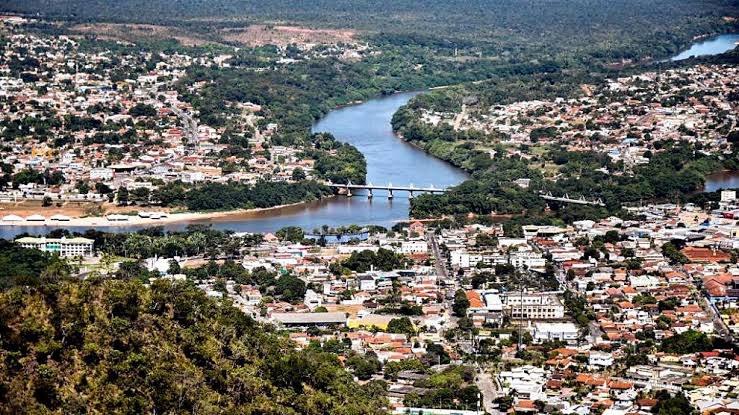
\includegraphics[width=0.8\linewidth]{barra.png}
    \caption{Foto da Cidade}
    \label{fig:cidade}
\end{figure}

Uma das figuras mais emblemáticas da região é o coronel inglês Percy Fawcett, que desapareceu em 1925 durante uma expedição na Serra do Roncador, enquanto buscava uma cidade perdida chamada Z. Esse desaparecimento misterioso inspirou filmes e livros ao redor do mundo, aumentando o fascínio pelas lendas da região. A Serra do Roncador é amplamente conhecida por seus mistérios e atrai inúmeros curiosos que buscam entender mais sobre o local. Existe um ``discoporto'' em Barra das Garças, que seria um suposto aeroporto para discos voadores, construído para facilitar o contato com seres de outros planetas. Segundo os relatos locais, há menções frequentes de avistamentos e aparições de luzes misteriosas que, para muitos, reforçam a crença na presença de vida extraterrestre na região.

A Gruta dos Pezinhos é outro local intrigante, conhecida por suas marcas petrificadas que muitos consideram um exemplo do misticismo local. Margherita de Tomas, jornalista e escritora italiana que estuda o desaparecimento de Fawcett, visitou a gruta e afirmou que os pés com diferentes números de dedos podem ser explicados como casos de polidactilia ou mesmo mutilações, aumentando ainda mais o caráter enigmático do local.

De acordo com a reportagem da BBC, os mistérios da região também envolvem lendas de intraterrenos - seres que vivem em cidades subterrâneas e que estão em constante vigilância para proteger seus domínios de possíveis invasores. Essas histórias, contadas por gerações, reforçam a crença de que há portais e caminhos secretos que levam a mundos escondidos abaixo da superfície. O coronel Percy Fawcett estava em busca desses mistérios quando desapareceu, e muitas das teorias locais apontam que ele poderia ter encontrado uma dessas entradas, levando ao seu desaparecimento.

% \begin{figure}[hbt]
%     \centering
%     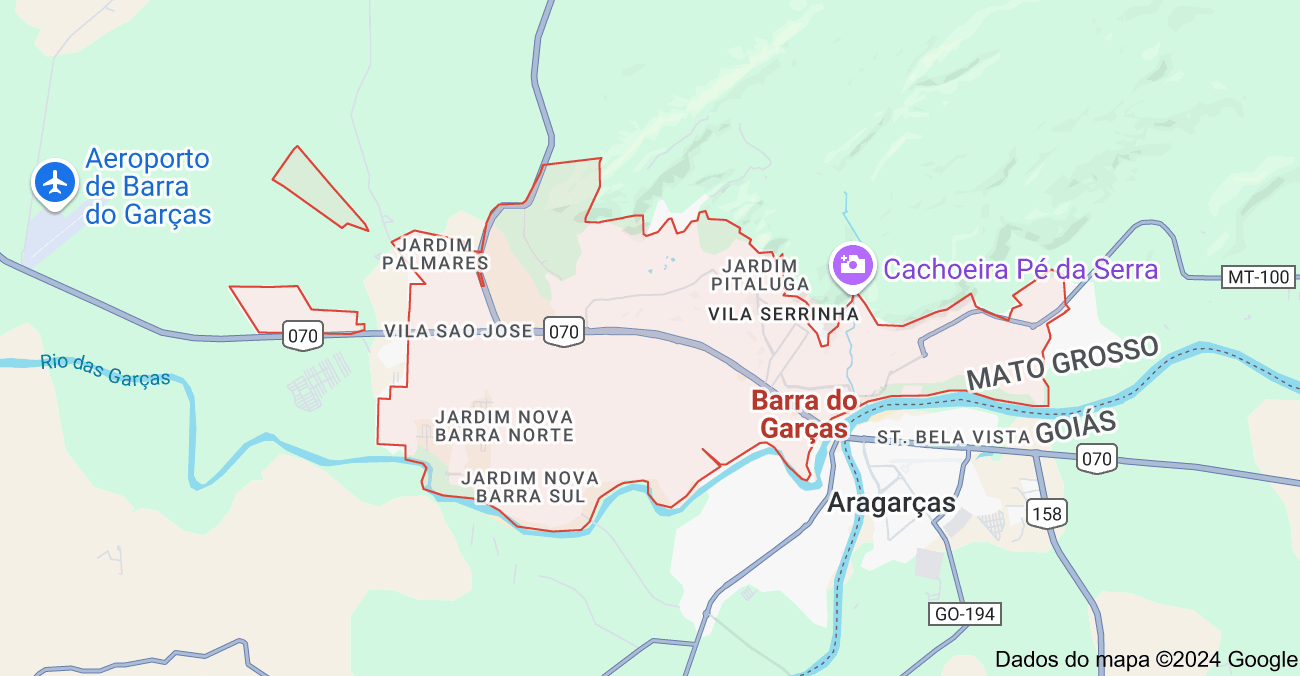
\includegraphics[width=0.5\linewidth]{barradasgarças.png}
%     \caption{Mapa de Barra das Garças}
%     \label{fig:mapa}
% \end{figure}

\section{Início}

Os agentes chegam de carro na cidade, às duas horas da tarde e com muita fome.
O carro não tem identificação, os agentes não podem usar de nenhum cargo oficial.


\chapter{A Missão}

\section{Objetivo: Verificar a Assombração no Cemitério}
A cidade de Barra das Garças, um destino turístico místico e esotérico na região Centro-Oeste do Brasil, é conhecida por suas paisagens naturais, como a Serra do Roncador e a confluência dos rios Araguaia e Garças. Mas é o Cemitério Municipal que tem chamado a atenção da ANVESN nas últimas semanas. Diversos relatos de avistamentos de uma figura espectral circulam entre os moradores, especialmente durante a noite. Testemunhas afirmam que o fantasma, possivelmente de uma mulher, aparece flutuando entre as lápides, emitindo uma leve luminescência azulada e pronunciando palavras incompreensíveis.

A missão inicial dos agentes é investigar essas ocorrências no cemitério, determinar a veracidade dos relatos e, se confirmado o fenômeno, conter a presença sobrenatural para evitar um possível aumento no turismo sensacionalista ou na histeria local. A ANVESN já identificou várias testemunhas dispostas a fornecer depoimentos sobre a aparição.

\section{Briefing da Cidade: Barra das Garças}
Barra das Garças é uma cidade de aproximadamente 61 mil habitantes, conhecida não apenas por sua beleza natural, mas também pela rica cultura folclórica e histórias sobrenaturais. A cidade é famosa por lendas locais sobre portais dimensionais e atividades alienígenas, ganhando reputação como um ponto místico e de avistamento de OVNIs. Com o desaparecimento misterioso do coronel inglês Percy Fawcett em 1925, enquanto explorava a Serra do Roncador em busca da lendária Cidade Z, a cidade tornou-se um lugar ainda mais intrigante para curiosos e místicos.

A cidade conta com diversos estabelecimentos que exploram essa atmosfera, como o jornal sensacionalista ``O Araguaia'' e o Bar ``Lua Cheia'', onde histórias sobre o cemitério e aparições locais são discutidas com entusiasmo. Esse interesse no sobrenatural faz parte da identidade local, mas também traz desafios para a ANVESN em conter possíveis excessos e histeria.

\section{Informações Práticas e Rumores Místicos}
\begin{itemize}
    \item \textbf{Localização do Cemitério}: Situado no perímetro norte da cidade, o cemitério é uma área bastante arborizada e pouco iluminada, especialmente à noite, o que contribui para o clima de mistério. A entrada principal é vigiada por uma guarda noturna, que também relata sons estranhos e aparições de luzes.

    \item \textbf{Horário dos Avistamentos}: Os relatos de aparição do fantasma variam, mas a maioria das testemunhas indica que ele surge entre meia-noite e duas da manhã, período conhecido na cidade como a ``Hora Azul''. Moradores mais velhos dizem que este é o momento em que o véu entre os mundos é mais fino, facilitando manifestações sobrenaturais.

    \item \textbf{Fofoqueira Local, Dona Lurdinha}: Dona Lurdinha, proprietária da venda de quitutes na Praça Central, tem muitos relatos sobre o cemitério e garante que o fantasma é o espírito de uma mulher que perdeu seu amor na Serra do Roncador. Ela afirma que a assombração busca por algo, mas nunca encontra, repetindo a jornada todas as noites. Dona Lurdinha é uma fonte constante de rumores e gosta de alimentar o mistério em suas conversas com os visitantes.

    \item \textbf{Conexão com a Igreja de São Miguel}: Alguns moradores associam o espírito a eventos ocorridos na Igreja de São Miguel, onde, há muitos anos, foram registrados exorcismos e rituais para proteção da cidade. A igreja, localizada próxima ao cemitério, é frequentada por devotos que acreditam que as almas perturbadas do cemitério são atraídas pela energia do local. O padre atual, no entanto, nega qualquer envolvimento direto com o fenômeno e se recusa a comentar o assunto.

    \item \textbf{O Jornal ``O Araguaia'' e sua Cobertura}: ``O Araguaia'' é conhecido por exagerar ou até fabricar histórias para aumentar o turismo místico na cidade. Recentemente, publicou uma matéria detalhada sobre o fantasma do cemitério, associando-o a portais interdimensionais e teorias de conspiração. Essa matéria aumentou a atenção sobre o caso, e a ANVESN suspeita que as descrições exageradas estejam contribuindo para a histeria.

    \item \textbf{Relatos de Luzes Misteriosas na Serra}: Além do cemitério, há frequentes relatos de luzes inexplicáveis na Serra do Roncador, que muitos moradores acreditam estar ligadas ao espírito do cemitério. Algumas teorias populares afirmam que essas luzes guiam almas perdidas de volta ao cemitério, alimentando ainda mais a aura de mistério.

    \item \textbf{Sinais de Atividade Esotérica na Região}: A região tem sido alvo de atividades de grupos esotéricos, que realizam rituais e vigílias à noite, afirmando que o cemitério é um ponto de contato com outras dimensões. Esse movimento atrai curiosos e gera polêmicas locais, pois há aqueles que acreditam que esses grupos despertam energias que deveriam permanecer adormecidas.

\end{itemize}

\section{Ação Inicial da Missão}
Os agentes da ANVESN devem chegar ao cemitério antes do horário crítico de meia-noite, realizando uma varredura inicial para garantir que não haja pessoas ou grupos esotéricos na área. É importante que os agentes estabeleçam contato com a guarda noturna e com eventuais testemunhas nas proximidades para obter mais informações.

Caso o fantasma se manifeste, os agentes devem proceder com medidas de contenção e, se necessário, exorcismo, para selar qualquer presença sobrenatural. A missão primária é observar e relatar, mas a ANVESN também autoriza os agentes a usarem equipamentos especiais de detecção de atividades ectoplásmicas e selos de contenção, caso o fenômeno apresente risco aos cidadãos de Barra das Garças.



\chapter{Locações e Descrição}

Essas são locações e personagens que podem sempre ser encontrados nelas.

\section{Praça Central e a Venda da D. Lurdinha}

A praça central de Barra das Garças é um dos pontos mais movimentados e pitorescos da cidade, cercada por árvores frondosas e canteiros floridos. 

\subsection{A venda de D. Lurdinha}

No coração da praça, encontra-se a famosa venda da D. Lurdinha, uma simpática senhora que vende quitutes regionais e doces caseiros, tornando-se uma referência de acolhimento para moradores e turistas. 
\dperson{D. Lurdinha, proprietária da venda}{
D. Lurdinha é uma personagem singular: em sua infância, afirma ter testemunhado um misterioso objeto cair do céu na floresta próxima, um evento que ela relembra com detalhes vívidos. Ela compartilha essas histórias com quem a visita, afirmando que algo incomum ronda a cidade há décadas. D. Lurdinha é bem-humorada, com um toque de mistério, e sempre parece saber mais do que revela, tornando-se uma importante fonte de informações para os agentes.}{}  


\begin{figure}[hbt]
    \centering
    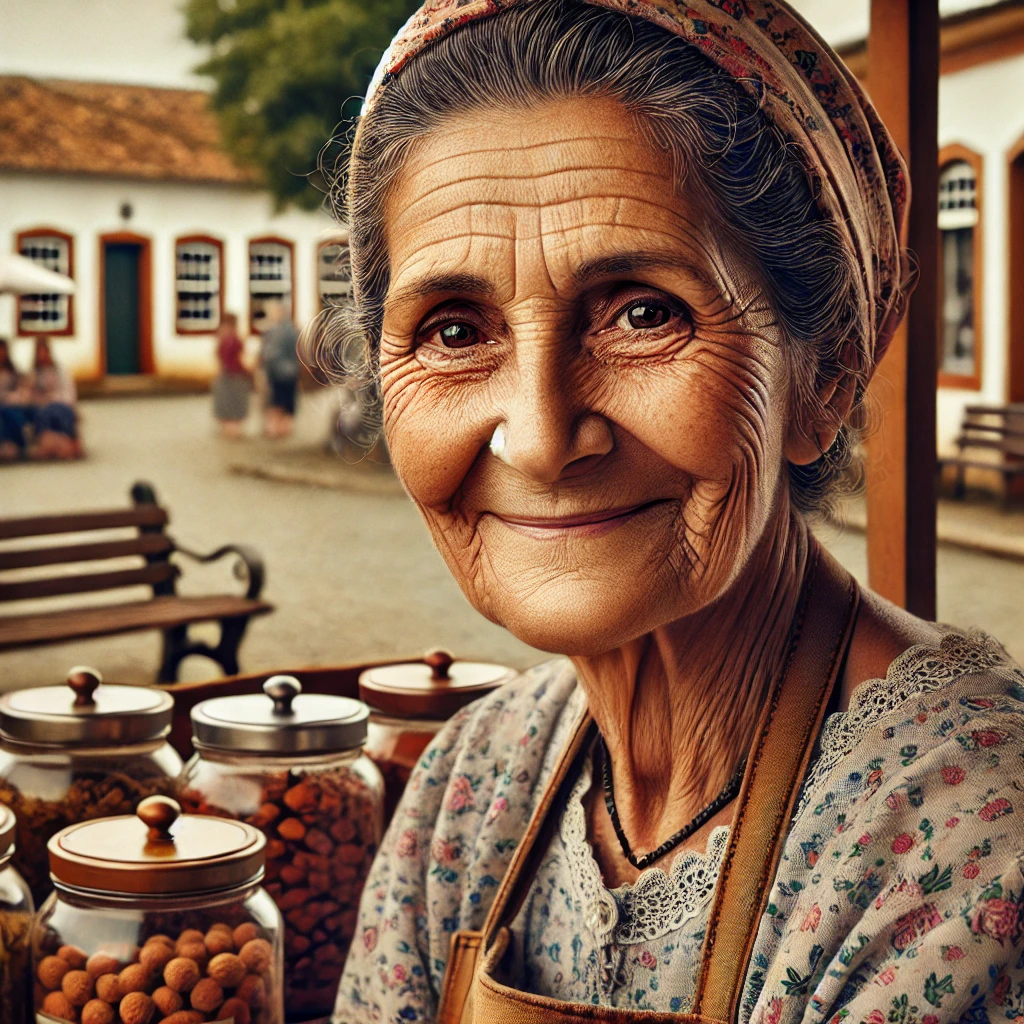
\includegraphics[width=0.5\linewidth]{lurdinha.png}
    \caption{D. Lurdinha}
    \label{figfantasma}
\end{figure}

\subsection{Os jogadores de dominó}


Ao lado da venda, há uma mesa de dominó sempre ocupada por quatro figuras locais, que diariamente jogam e discutem as histórias e mistérios da cidade:

\begin{personagem}[Personagens]
\begin{itemize}
    \item \textbf{Seu Zeca, o Barbeiro}: Um veterano que conhece todos na cidade e costuma afirmar que o cemitério e as cavernas escondem mais do que simples lendas. Ele é observador e já ouviu falar dos intraterrenos.
    \item \textbf{Dona Rosa, a Parteira}: Mulher sábia e respeitada, Dona Rosa acredita no sobrenatural e diz que já viu luzes estranhas na Serra do Roncador. Ela também já fez partos que, segundo ela, foram acompanhados por visões de figuras sombrias.
    \item \textbf{Tonico, o Pescador}: Com sua pele queimada de sol, Tonico diz ter visto OVNIs sobre o rio Araguaia e acredita que são entidades pacíficas. Ele desconfia de Bento e de sua relação com os intraterrenos.
    \item \textbf{Pedro, o Poeta}: Pedro é um boêmio que adora contar histórias poéticas e teorias sobre os portais para outras dimensões. Ele acredita que o ET que caiu está apenas de passagem e tem uma conexão mística com a cidade.
\end{itemize}
\end{personagem}

Cada um deles tem uma personalidade única e suas próprias teorias sobre os eventos misteriosos de Barra das Garças, proporcionando informações e novas perspectivas para os agentes.

\begin{figure}[hbt]
    \centering
    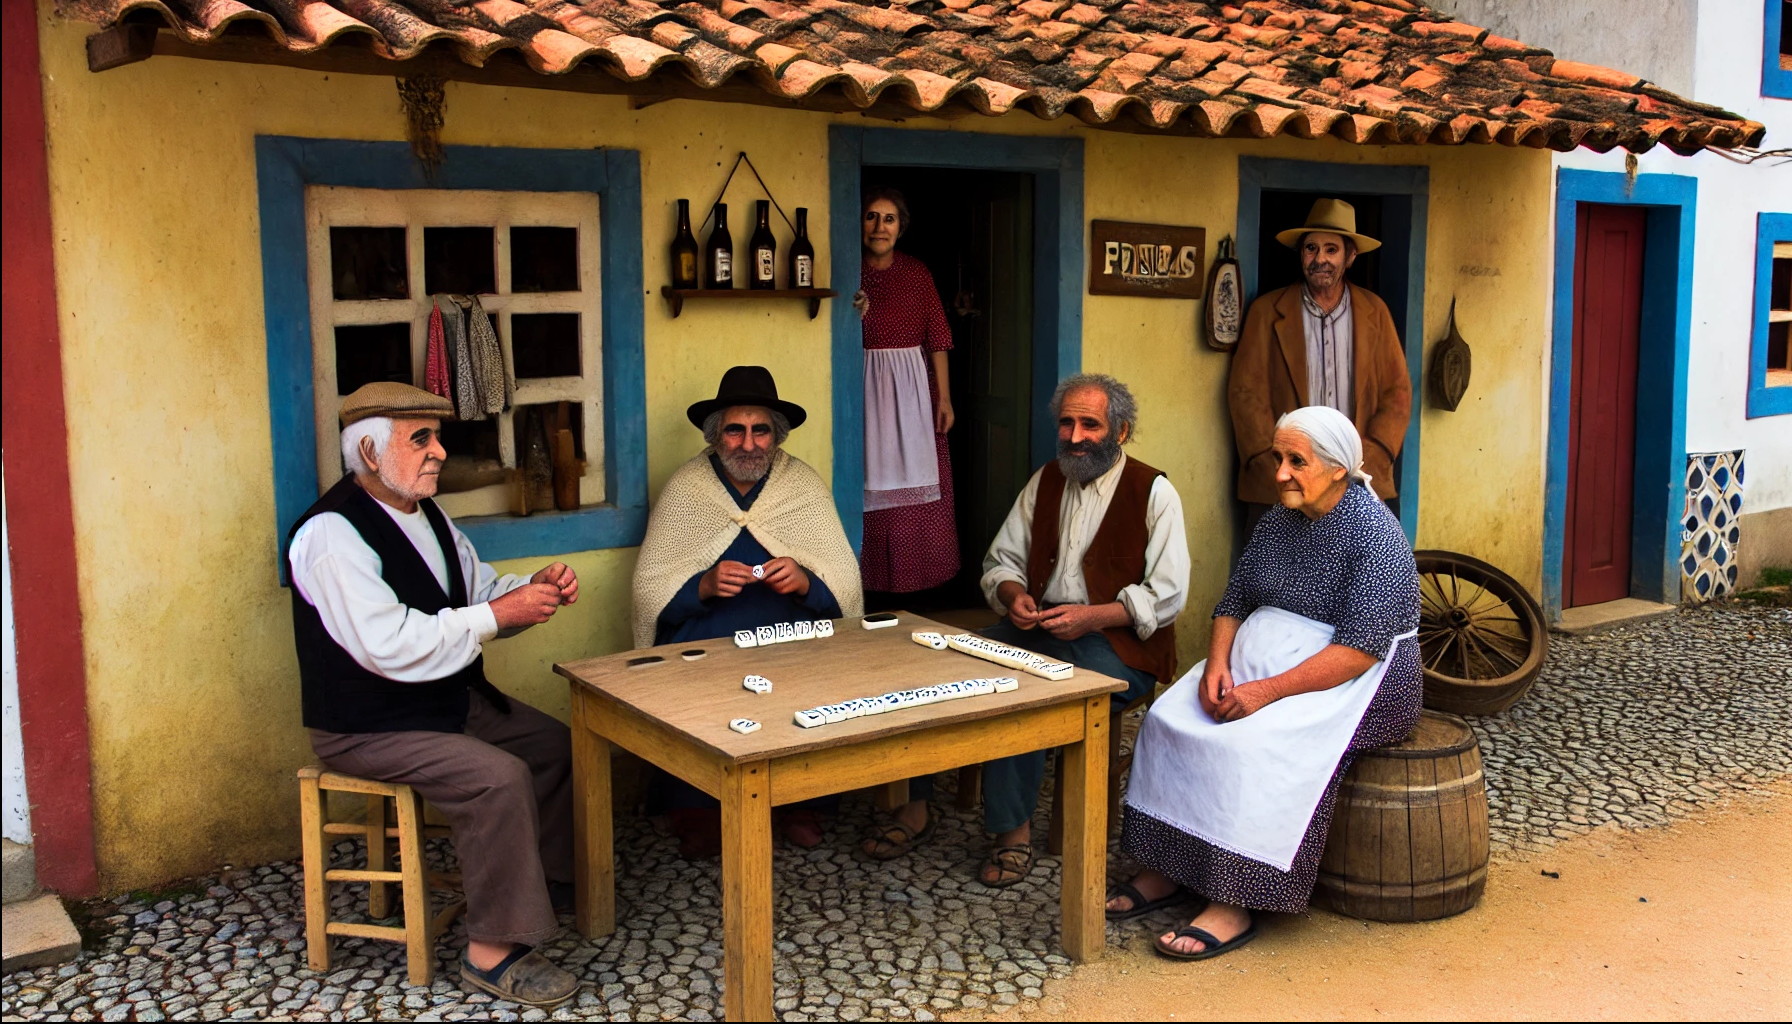
\includegraphics[width=0.5\linewidth]{domino.png}
    \caption{Caption}
    \label{fig:enter-label}
\end{figure}

\section{Interior da Entrada Secreta para o Intraterra}


O acesso ao Intraterra leva a uma caverna com quatro salas, construídas com arquitetura rudimentar. No final do túnel está a \textbf{Sala do Portal}, mas sua porta está trancada por dentro e é impossível entrar. Ela parece ser usada para monitoramento ou controle remoto e possui uma estranha vibração.

\subsection{Salas da Caverna}

\begin{itemize}
    \item \textbf{Sala de Monitoramento}: Contém monitores antigos e uma mesa com anotações em uma linguagem desconhecida. Os intraterrenos usam essa sala para vigiar atividades da superfície. \textbf{Documentos Relacionados}: Notas descrevendo encontros regulares entre humanos da superfície e intraterrenos, incluindo detalhes sobre um grupo liderado por Bento. Essas anotações mencionam o fornecimento de informações sobre atividades na cidade e trocas de recursos em pontos específicos da floresta.
    \item \textbf{Sala de Armas}: Armas primitivas e equipamentos de defesa. Agentes podem reconhecer o estilo similar a relíquias de guerra humanas.
    \item \textbf{Sala de Conferência}: Um espaço para reuniões com uma grande mesa de pedra. Há gravuras nas paredes retratando batalhas antigas com figuras humanoides. \textbf{Documentos Relacionados}: Relatórios sobre estratégias de defesa contra "invasores do céu", que provavelmente referem-se a seres como o ET. O documento também sugere uma aliança de apoio com grupos humanos na superfície.
    \item \textbf{Sala do Portal (trancada)}: Localizada no final do túnel, com portas grossas de pedra que só podem ser abertas por dentro. Os agentes não conseguem entrar, mas devem monitorar a área, pois há sinais de uso recente.
\end{itemize}

\section{Discódromo}

O discódromo sedia uma festa “Mística”, atraindo seguidores de Bento e curiosos sobre o paranormal.

\subsection{Itens e Pistas}

\begin{itemize}
    \item \textbf{Broche de Intraterrenos}: Um pequeno broche em formato de criatura subterrânea, usado pelos aliados de Bento.
    \item \textbf{Convite para Reunião Secreta}: Panfleto sobre uma reunião organizada por Bento e os intraterrenos para discutir a “proteção” da cidade.
\end{itemize}


\begin{personagem}
\subsection{Cláudia, a DJ} Sabe dos encontros de Bento e pode compartilhar informações sobre as atividades do grupo de conspiradores. Ela também ouviu rumores sobre a cidade perdida e diz que alguns dos frequentadores da festa falam sobre ela como um lugar que deve ser evitado a todo custo.
\end{personagem}



\section{Prefeitura}

A prefeitura abriga os registros históricos e é uma importante fonte de dados sobre as atividades incomuns na cidade.

\subsection{Itens e Pistas}

\begin{itemize}
    \item \textbf{Relatos de Avistamentos}: Arquivos sobre luzes e figuras misteriosas vistas na cidade.
    \item \textbf{Mapa Geológico}: Um mapa com informações sobre cavernas e túneis que parecem corresponder aos relatos de eventos recentes.
    \item \textbf{Documentos de Encontro}: Relatórios que descrevem um grupo de residentes da cidade em comunicação com figuras "misteriosas" que se escondem nos túneis subterrâneos. Estes documentos mencionam promessas de proteção em troca de informações e recursos. Há também menção a uma suposta relação entre a cidade perdida e os espíritos obsessores, sugerindo que esses seres possam estar manipulando alguns dos eventos recentes.
\end{itemize}


\begin{personagem}
\subsubsection{Prefeito Antônio de Souza}
\textbf{Nome:} \pindex{Antônio de Souza}
\textbf{Idade:} 58 anos  
\textbf{Descrição:}  
Prefeito Antônio é um homem reservado, que governa a cidade de Barra das Garças com um estilo moderado e diplomático. Ele possui uma postura séria e sempre usa ternos formais, embora mantenha um ar acolhedor para lidar com os cidadãos. O prefeito se preocupa genuinamente com o bem-estar da cidade, mas enfrenta dificuldades para conter os crescentes rumores sobrenaturais. Antônio é casado com a filha do espírito maternal que assombra o cemitério, e o relacionamento com a esposa o torna um homem protetor e discreto, sempre atento ao bem-estar dela.

\textbf{Traços de Personalidade:}
\begin{itemize}
    \item \textbf{Calmo e Diplomático}: Prefere manter a ordem e evita confrontos diretos.
    \item \textbf{Reservado sobre Assuntos Sobrenaturais}: Não gosta de alimentar boatos, mas sente que está perdendo o controle dos rumores.
    \item \textbf{Protetor da Esposa}: Sua esposa tem prioridade em suas decisões, e ele tenta protegê-la de qualquer situação que possa causar-lhe estresse.
\end{itemize}
\end{personagem}
\begin{personagem}  
\subsubsection{Esposa do Prefeito - Helena de Souza}

\textbf{Nome:} \pindex{Helena de Souza}
\textbf{Idade:} 39 anos  
\textbf{Descrição:}  
Helena é uma mulher amável e bondosa, conhecida por sua gentileza e disposição para ajudar as pessoas da cidade. Ela não sabe que sua mãe faleceu quando ainda era uma criança e que o espírito dela a protege até hoje. Casada com o prefeito, Helena mantém uma presença discreta e evita qualquer atenção pública, preferindo apoiar as causas da cidade por trás das cortinas. Ela tem um forte vínculo com o cemitério, embora não compreenda o porquê.

\textbf{Traços de Personalidade:}
\begin{itemize}
    \item \textbf{Gentil e Caridosa}: É amada na cidade por seu comportamento altruísta.
    \item \textbf{Reservada}: Evita eventos públicos e mantém uma vida privada.
    \item \textbf{Ligação com o Sobrenatural}: Sente-se atraída pelo cemitério e locais místicos, mesmo sem saber o motivo.
\end{itemize}
\end{personagem}
\begin{personagem}  

\subsubsection{Subprefeito - Carlos Menezes}

\textbf{Nome:} Carlos Menezes  
\textbf{Idade:} 46 anos  
\textbf{Descrição:}  
Carlos é o subprefeito e uma figura de confiança do prefeito Antônio, conhecido por sua lealdade e eficiência. É um homem prático e pragmático, que cuida dos assuntos administrativos e apoia as iniciativas de desenvolvimento da cidade, especialmente no turismo. Carlos tem uma personalidade resoluta e é cético em relação ao sobrenatural, vendo os boatos como "superstições".

\textbf{Traços de Personalidade:}
\begin{itemize}
    \item \textbf{Eficiência e Pragmatismo}: Resolve os problemas da cidade com rapidez e precisão.
    \item \textbf{Lealdade Inquestionável}: Apoia as decisões do prefeito e faz de tudo para manter a cidade em ordem.
    \item \textbf{Cético ao Sobrenatural}: Considera os boatos sobrenaturais uma bobagem, útil apenas para turismo.
\end{itemize}
\end{personagem}
\begin{personagem}  
 
\subsubsection{Vereador - João "Joca" Alves}

\textbf{Nome:} João Alves, conhecido como "Joca"  
\textbf{Idade:} 42 anos  
\textbf{Descrição:}  
Joca é um vereador simples e próximo do povo, sempre preocupado com as necessidades dos moradores de Barra das Garças. Ele é simpático e amigável, mas extremamente cauteloso com as histórias sobrenaturais que circulam pela cidade. Joca acredita que os boatos causam mais problemas do que benefícios, e tenta moderar as atitudes de Miguel para não alarmar a população.

\textbf{Traços de Personalidade:}
\begin{itemize}
    \item \textbf{Amigável e Popular}: Conhecido por sua proximidade com a comunidade.
    \item \textbf{Prudente e Conservador}: Não gosta de exageros em relação às histórias místicas da cidade.
    \item \textbf{Conflito com Miguel}: Muitas vezes tenta impedir os planos de Miguel para manipular as lendas em benefício próprio.
\end{itemize}
\end{personagem}
\begin{personagem}  
 \subsubsection{Dona Cláudia, a Secretária da Prefeitura}
 
 Conhece bem a história da cidade e suspeita das atividades de Bento. Ela revela que Bento tem buscado mapas das cavernas da região. Dona Cláudia também menciona que muitos registros antigos falam sobre uma cidade perdida e o aeroporto alienígena, frequentemente citados nos documentos mais misteriosos da prefeitura.
\end{personagem}
 
\section{Biblioteca Municipal de Barra do Garças}

\textbf{Descrição:}  
A Biblioteca Municipal de Barra do Garças é uma construção histórica de estilo colonial, situada no coração da cidade, próxima à praça principal. Com paredes de tijolos aparentes e grandes janelas de vidro, o prédio transmite uma atmosfera de mistério e tranquilidade, atraindo tanto moradores quanto visitantes em busca de informações sobre a história e os mitos da região. A biblioteca possui uma coleção variada que abrange desde obras literárias clássicas até documentos sobre o folclore e os eventos sobrenaturais locais.

No interior, a biblioteca é dividida em várias áreas de consulta e pesquisa, com seções dedicadas a literatura geral, periódicos antigos e documentos históricos. A estrutura interna é simples, mas o ambiente é acolhedor e repleto de detalhes místicos, como pequenos quadros com símbolos de proteção e estantes cuidadosamente organizadas. A biblioteca também oferece acesso à internet para consultas digitais, permitindo que os visitantes acessem bancos de dados online e recursos de pesquisa que complementam as investigações locais.

\subsection{Áreas Principais da Biblioteca}

\begin{itemize}
    \item \textbf{Área de Leitura Pública}  
    Um salão amplo e iluminado, com mesas de leitura de madeira dispostas em filas, onde os visitantes podem consultar livros e materiais de estudo. Esta área possui estantes organizadas por categorias que incluem literatura, ciências e mitologia, com uma seção dedicada ao folclore brasileiro e às lendas de Barra do Garças, muito popular entre os visitantes.

    \item \textbf{Arquivo de Documentos Históricos}  
    A seção de documentos históricos está disponível apenas para pesquisadores autorizados e contém registros raros, como mapas detalhados da região, jornais antigos, diários de exploradores e relatos de avistamentos de luzes e criaturas misteriosas. Este arquivo é guardado com segurança, e somente funcionários da biblioteca têm acesso direto às prateleiras, que são fechadas com grades de ferro.

    \item \textbf{Sala de Mapas e Documentação Local}  
    Ao lado do arquivo histórico, esta sala é especializada em mapas e documentos específicos de Barra do Garças e seus arredores. Muitos dos mapas contêm anotações sobre a Serra do Roncador e pontos de interesse onde ocorreram avistamentos misteriosos, e a sala é um ponto valioso para aqueles que investigam atividades sobrenaturais.

    \item \textbf{Seção de Periódicos e Jornais Antigos}  
    Esta seção abriga edições antigas de jornais locais, contendo matérias sobre eventos notórios como o desaparecimento do coronel Percy Fawcett e os primeiros relatos de avistamentos de intraterrenos. Muitos visitantes e pesquisadores buscam essa seção para entender a cronologia dos acontecimentos misteriosos da região.

    \item \textbf{Estação de Acesso à Internet}  
    A biblioteca oferece computadores com acesso à internet para consultas e pesquisas online. Esta área permite que os visitantes acessem bancos de dados, registros públicos, e realizem investigações que vão além dos arquivos físicos. Os computadores são frequentemente utilizados por estudantes e pesquisadores, e alguns visitantes optam por investigar lendas urbanas e teorias conspiratórias por meio de blogs e websites de conteúdo esotérico.
\end{itemize}

\subsection{Personagens da Biblioteca}

\begin{personagem}  
\paragraph{Dona Irene Silva – Bibliotecária Chefe}  
\textbf{Idade:} 62 anos  
\textbf{Descrição:}  
Dona Irene é a responsável pela organização e preservação do acervo da biblioteca. Ela é uma mulher de semblante sereno, sempre disposta a ajudar, mas também reservada sobre as informações que compartilha. Irene conhece profundamente a história de Barra do Garças e as lendas locais, e administra o arquivo histórico com zelo. Embora seja cautelosa, Irene compartilha informações valiosas com aqueles que demonstram interesse genuíno pelos mistérios da cidade.

\textbf{Traços de Personalidade:}
\begin{itemize}
    \item \textbf{Conhecedora das Lendas Locais}: Irene é uma fonte de informações sobre o folclore e os eventos misteriosos da região.
    \item \textbf{Cuidadosa e Atenciosa}: Ela cuida pessoalmente dos arquivos históricos e garante que somente pessoas autorizadas tenham acesso.
    \item \textbf{Reservada e Prudente}: Compartilha informações somente com aqueles que demonstram um interesse genuíno e respeitoso.
\end{itemize}
\end{personagem}
\begin{personagem}  
\paragraph{Gabriel Costa – Jovem Auxiliar}  
\textbf{Idade:} 24 anos  
\textbf{Descrição:}  
Gabriel é o assistente da biblioteca, um estudante de história curioso e apaixonado pelas lendas de Barra do Garças. Ele é responsável por organizar os arquivos e auxiliar os visitantes. Gabriel se interessa pelas teorias sobrenaturais e conspirações locais, e frequentemente direciona os visitantes para seções relevantes. Seu entusiasmo pelo misticismo local torna-o uma ajuda valiosa para quem busca informações sobre o folclore.

\textbf{Traços de Personalidade:}
\begin{itemize}
    \item \textbf{Curioso e Prestativo}: Gabriel adora compartilhar teorias e orientar os visitantes sobre temas misteriosos.
    \item \textbf{Entusiasta de Conspirações}: Ele está sempre atualizado sobre teorias locais e gosta de discutir histórias místicas.
    \item \textbf{Leal a Dona Irene}: Gabriel respeita muito a bibliotecária chefe e ajuda a manter a organização dos arquivos históricos.
\end{itemize}
\end{personagem}

\subsection{Itens e Pistas na Biblioteca}

\begin{itemize}
    \item \textbf{Diário de Joaquim Brandão}: Guardado na seção de documentos históricos, este diário contém informações sobre a investigação de Joaquim antes de seu assassinato, incluindo suas suspeitas sobre Bento Silva.

    \item \textbf{Mapa Anotado da Cidade e da Serra do Roncador}: Na sala de mapas, este documento possui marcações feitas por Joaquim em locais onde Bento realizava encontros suspeitos. As marcações ajudam a traçar os movimentos de Bento e a localizar pontos de interesse para investigação.

    \item \textbf{Arquivo de Periódicos sobre Avistamentos}: Na seção de periódicos e jornais antigos, os personagens podem acessar reportagens e relatos de eventos sobrenaturais que datam de várias décadas, fornecendo uma linha do tempo dos fenômenos misteriosos.

    \item \textbf{Carta Anônima sobre Bento}: Nos documentos antigos, os personagens encontram uma carta endereçada a Joaquim alertando sobre o perigo de investigar Bento, sugerindo que ele poderia estar envolvido com forças "fora deste mundo".
\end{itemize}

\subsection{Interação com a Biblioteca}

A Biblioteca Municipal é um recurso essencial para os personagens que investigam a história e os mistérios de Barra do Garças. Com o auxílio de Dona Irene e Gabriel, os personagens podem descobrir documentos valiosos, acessar a internet para expandir suas investigações, e obter informações que conectam eventos do passado às atividades de Bento Silva e outros envolvidos. O ambiente da biblioteca, repleto de histórias e lendas, incentiva a exploração cuidadosa e oferece várias pistas para desvendar os mistérios da cidade.



\section{Floresta}

Nas margens da cidade e perto do cemitério, há uma área de mata densa onde a nave do ET está escondida. Camuflada com tecnologia avançada, ela emite uma leve vibração detectável apenas com equipamentos especiais.

\subsection{Itens e Pistas}

\begin{itemize}
    \item \textbf{Nave do ET}: Um objeto camuflado, com aparência que se mistura ao ambiente da floresta. A nave só pode ser vista por quem usa equipamento de detecção de radiação ou frequências incomuns.
    \item \textbf{Peça Desgastada}: Uma parte avariada da nave que o ET pede aos agentes para substituir. A peça deve ser recuperada dos intraterrenos.
\end{itemize}


\begin{personagem}  

\begin{itemize}
    \item \textbf{ET}: Explica aos agentes que sua nave sofreu danos e precisa de uma peça específica, que os intraterrenos levaram. Ele pede ajuda para recuperá-la antes que os intraterrenos consigam usá-la contra ele.
\end{itemize}
\end{personagem}

subsection{O Hotel e seus Habitantes}

\subsubsection{Hotel Encanto do Araguaia}

\textbf{Descrição:}  
O Hotel Encanto do Araguaia é o mais antigo da cidade, um casarão colonial reformado que atrai turistas interessados nos mistérios de Barra das Garças. Com uma decoração rústica e tradicional, o hotel preserva um charme antigo, mas também é conhecido por sons misteriosos e fenômenos incomuns que ocorrem à noite. A cozinha do hotel é um ponto de atividades inexplicáveis, e muitos hóspedes já relataram ouvir barulhos estranhos e passos quando tudo deveria estar em silêncio.

\begin{personagem}  
\subsubsection{Dona Celina – Proprietária do Hotel}

\textbf{Nome:} Celina Marques  
\textbf{Idade:} 63 anos  
\textbf{Descrição:}  
Dona Celina é uma senhora elegante e carismática, conhecida por sua hospitalidade e atenção aos detalhes. Ela administra o hotel com dedicação, e embora tenha consciência dos fenômenos que ocorrem à noite, evita discutir o assunto com os hóspedes para não assustá-los. Celina é uma defensora das tradições locais e valoriza a cultura da cidade, mas guarda segredo sobre as atividades estranhas no hotel.

\textbf{Traços de Personalidade:}
\begin{itemize}
    \item \textbf{Hospitaleira e Elegante}: Recebe todos com um sorriso e faz questão de cuidar bem de cada hóspede.
    \item \textbf{Discreta sobre o Sobrenatural}: Prefere não alimentar rumores e ignora os fenômenos quando pode.
    \item \textbf{Ligada à Cultura Local}: Ama a cidade e as tradições locais, contribuindo para preservar a imagem do hotel.
\end{itemize}
\end{personagem}
\begin{personagem}  
\subsubsection{Poltergeist da Cozinha}

\textbf{Descrição:}  
Todas as noites, barulhos inexplicáveis, como talheres se movendo e portas de armários batendo, são ouvidos na cozinha do hotel. Pratos são deixados fora de lugar, e utensílios caem das prateleiras. Os hóspedes curiosos que investigam a cozinha durante a noite frequentemente encontram a cozinha em desordem, mas nunca veem o causador do distúrbio. O poltergeist parece mais brincalhão do que perigoso, mas cria desconforto entre os funcionários e hóspedes.

\textbf{Características do Poltergeist:}
\begin{itemize}
    \item \textbf{Ruídos Altos e Inesperados}: Batidas, passos e barulhos de objetos sendo arrastados.
    \item \textbf{Desordem Visível}: Talheres e pratos mudam de lugar misteriosamente durante a noite.
    \item \textbf{Presença Inquietante}: Provoca sustos, mas não causa danos físicos, preferindo a desordem e o desconforto.
\end{itemize}
\end{personagem}
\begin{personagem}  
\subsubsection{Arrumadeira Tereza}

\textbf{Nome:} Tereza dos Santos  
\textbf{Idade:} 45 anos  
\textbf{Descrição:}  
Tereza é uma mulher de personalidade forte, que cuida do hotel com rigor e eficiência. Ela é uma presença firme, sempre pronta para repreender qualquer um que bagunce os quartos ou corredores. Tereza não se intimida com os boatos de assombração e acredita que o poltergeist é apenas "mais uma coisa" para organizar. Os hóspedes a consideram um pouco rígida
\end{personagem}


\subsection{A Lagoa do Poder}

\textbf{Descrição:}  
A Lagoa do Poder é um local de intensa energia mística, cercado por vegetação densa e distante das trilhas mais frequentadas. A água da lagoa é escura e reflete o céu de forma quase sobrenatural, parecendo mais profunda e misteriosa do que realmente é. Segundo a lenda, a lagoa possui poderes de amplificação espiritual e é usada em rituais por feiticeiros e místicos. Dizem que em noites de lua cheia, a lagoa exibe uma névoa prateada que cobre a água, e quem a toca sente uma onda de energia percorrer o corpo.

\textbf{Características da Lagoa:}  
\begin{itemize}
    \item \textbf{Efeitos Energéticos}: Muitos dizem sentir uma energia poderosa ao redor da lagoa, como se ampliasse percepções e intuições.
    \item \textbf{Lugar de Rituais}: É usada por feiticeiros e bruxas locais para rituais de proteção e conexão com o sobrenatural.
    \item \textbf{Aparições Noturnas}: Estranhas figuras e luzes são vistas em noites de lua cheia, intensificando o mistério da lagoa.
\end{itemize}

\section{Delegacia de Barra do Garças}


A Delegacia de Barra do Garças é um pequeno prédio de tijolos à vista, localizado próximo à praça central da cidade. Com uma fachada discreta, o edifício possui apenas algumas salas para acomodar a equipe policial, um depósito de evidências e uma cela temporária para deter suspeitos. O ambiente é simples e funcional, com móveis desgastados e arquivos antigos empilhados nas prateleiras. A delegacia enfrenta falta de recursos, como muitas outras em pequenas cidades, e conta com uma equipe reduzida. No entanto, o trabalho dos oficiais locais é marcado pela familiaridade com a população e uma abordagem mais pessoal na resolução de casos.

A delegacia está constantemente ocupada com pequenos incidentes locais, como brigas de bar e desentendimentos familiares, mas os rumores sobre atividades sobrenaturais e o aumento de avistamentos de luzes estranhas têm atraído a atenção de algumas figuras inusitadas, levando os policiais a lidarem com novos desafios. Embora alguns policiais sejam céticos quanto às histórias de assombrações e ETs, há uma curiosidade crescente, especialmente entre os mais jovens.

\subsection{Personagens da Delegacia}

\begin{personagem}  
\paragraph{Delegado Pedro Antunes}  
\textbf{Idade:} 48 anos  
\textbf{Descrição:}  
O Delegado Pedro Antunes é o responsável pela delegacia de Barra do Garças. Um homem de presença imponente e experiência na área de segurança, ele mantém uma postura séria e discreta em relação aos rumores sobrenaturais. Pedro é um pragmático, focado em manter a ordem na cidade e evitar alarmismos. Contudo, ele tem um conhecimento detalhado sobre as lendas locais, pois nasceu e cresceu em Barra do Garças, e tem suas próprias teorias sobre os fenômenos, embora prefira não discuti-las abertamente.

\textbf{Traços de Personalidade:}
\begin{itemize}
    \item \textbf{Sério e Discreto}: Prefere lidar com assuntos de maneira formal e raramente se deixa envolver emocionalmente nos casos.
    \item \textbf{Protetor da Comunidade}: Sempre procura resolver conflitos sem atrair atenção negativa para a cidade.
    \item \textbf{Curioso em Relação às Lendas}: Apesar de cético, conhece bem as lendas locais e acompanha os relatos com interesse discreto.
\end{itemize}
\end{personagem}
\begin{personagem}  
\paragraph{Investigador Rafael "Rafa" Martins}  
\textbf{Idade:} 34 anos  
\textbf{Descrição:}  
Rafa é o principal investigador da delegacia e uma das figuras mais populares entre os moradores, graças à sua natureza amigável e ao talento para ouvir e conversar. Ele é um jovem entusiasmado, curioso, e já participou de investigações de casos sobrenaturais por interesse pessoal. Nos últimos meses, Rafa tem mantido um registro informal dos avistamentos de luzes e das histórias sobre o “ET”, e é conhecido por ser o policial que os moradores procuram quando querem discutir temas misteriosos. Ele tem um espírito de aventura e sempre busca entender o que há por trás das lendas.

\textbf{Traços de Personalidade:}
\begin{itemize}
    \item \textbf{Amigável e Acessível}: Rafa é popular na cidade e mantém uma relação próxima com os moradores.
    \item \textbf{Curioso e Investigativo}: Ele se interessa pelos eventos sobrenaturais e frequentemente pesquisa por conta própria.
    \item \textbf{Intuitivo}: É capaz de ler entre as linhas e tem talento para desvendar pistas pouco óbvias.
\end{itemize}
\end{personagem}
\begin{personagem}  
\paragraph{Sargento Luísa Silva}  
\textbf{Idade:} 42 anos  
\textbf{Descrição:}  
Sargento Luísa é uma policial experiente e disciplinada, com uma postura firme e uma personalidade prática. Ela tem pouco interesse pelas histórias sobrenaturais, considerando-as uma distração das questões reais de segurança. Luísa é rigorosa com o cumprimento das regras e é conhecida por seu senso de justiça. Cética em relação aos mistérios de Barra do Garças, vê-se como protetora da comunidade contra o medo e a paranoia, buscando sempre soluções racionais para os casos.

\textbf{Traços de Personalidade:}
\begin{itemize}
    \item \textbf{Rigorosa e Cética}: Luísa não se deixa influenciar por rumores e busca soluções racionais para cada caso.
    \item \textbf{Justa e Leal}: Tem um forte senso de dever e dedica-se a proteger os moradores.
    \item \textbf{Resistente a Pressões Externas}: Não é facilmente influenciada, mantendo uma postura firme.
\end{itemize}
\end{personagem}
\begin{personagem}  
\paragraph{Escrivão Paulo Farias}  
\textbf{Idade:} 50 anos  
\textbf{Descrição:}  
Paulo é o escrivão da delegacia e o responsável por manter todos os registros organizados, o que inclui arquivos de casos e depoimentos. Ele é um homem reservado e organizado, mas possui um lado curioso e está sempre atento às conversas dos colegas sobre os casos sobrenaturais. Paulo possui um vasto conhecimento sobre a história de Barra do Garças e, ao longo dos anos, compilou um acervo pessoal de documentos e reportagens sobre o folclore local, que ele mantém em segredo.

\textbf{Traços de Personalidade:}
\begin{itemize}
    \item \textbf{Organizado e Detalhista}: Responsável por garantir que todos os registros estejam sempre em ordem.
    \item \textbf{Curioso e Reservado}: Tem um acervo pessoal sobre o folclore local, mas compartilha apenas com quem confia.
    \item \textbf{Informante Secreto}: Às vezes revela pistas sobre lendas aos colegas, mas sempre de maneira sutil.
\end{itemize}
\end{personagem}
\begin{personagem}  
\paragraph{Patrulheiro João "Joãozinho" Alves}  
\textbf{Idade:} 27 anos  
\textbf{Descrição:}  
Joãozinho é o patrulheiro mais jovem da delegacia e bastante impressionável. Ele acredita firmemente nos fenômenos sobrenaturais que rondam Barra do Garças e é conhecido por suas histórias exageradas sobre encontros com fantasmas e figuras místicas. Os colegas da delegacia costumam brincar com ele sobre seus medos, mas Joãozinho acredita que a cidade é um ponto de encontro de forças misteriosas. Ele é amigável, prestativo e sempre disposto a compartilhar histórias assustadoras com quem estiver disposto a ouvir.

\textbf{Traços de Personalidade:}
\begin{itemize}
    \item \textbf{Impressionável e Supersticioso}: Acredita em cada história mística que ouve e não esconde isso.
    \item \textbf{Prestativo e Bem-Humorado}: Gosta de ajudar a comunidade e é conhecido por seu bom humor.
    \item \textbf{Narrador Entusiasta}: Sempre tem uma nova história assustadora para contar, encantando moradores e visitantes.
\end{itemize}
\end{personagem}

\subsubsection{Itens e Pistas na Delegacia}

\begin{itemize}
    \item \textbf{Relatórios de Avistamentos}: O Investigador Rafa mantém registros de depoimentos sobre aparições de luzes e figuras misteriosas, muitas vezes compilando as histórias dos moradores em um dossiê informal.
    \item \textbf{Arquivo de Casos Antigos}: O escrivão Paulo tem uma coleção de arquivos antigos que incluem lendas e relatos de atividades incomuns. Em meio aos registros, há menções a uma “cidade perdida” e a figuras misteriosas observadas na Serra do Roncador.
    \item \textbf{Mapa de Avistamentos Recorrentes}: Na sala de investigações, há um mapa com marcas em locais onde avistamentos de luzes foram reportados, muitos dos quais próximos ao cemitério e à Serra Azul.
\end{itemize}

\section{Jornal ``O Araguaia''}

 
``O Araguaia'' é o principal jornal de Barra das Garças, de propriedade do vereador Miguel Rocha. Em circulação há mais de 30 anos, o jornal é conhecido por sua postura conservadora e pelo tom sensacionalista, muitas vezes explorando o folclore e os rumores sobrenaturais da cidade para atrair leitores e fomentar o turismo. Miguel Rocha vê o jornal como uma ferramenta essencial para manipular a opinião pública e promover suas próprias ideias, especialmente o aumento do turismo baseado em lendas locais. 

O jornal possui uma pequena equipe de jornalistas que, embora tenham visões e motivações diferentes, ajudam a construir a narrativa editorial de Miguel, resultando em um periódico com matérias curiosas, mas muitas vezes incompletas ou enviesadas.


\subsection{Vereador - Miguel Rocha}

\textbf{Nome:} Miguel Rocha  
\textbf{Idade:} 53 anos  
\textbf{Descrição:}  
Miguel é um dos vereadores mais influentes de Barra das Garças e tem ideias polêmicas sobre o uso de lendas e boatos para impulsionar o turismo. Ele é o principal criador do plano de "notícias" sobrenaturais e divulga histórias de avistamentos e atividades místicas para atrair visitantes. Miguel é manipulador e astuto, sempre atento aos ganhos financeiros que pode obter com o aumento do turismo.

Como proprietário de ``O Araguaia'', Miguel usa o jornal como uma plataforma para promover seu próprio interesse de manipular o turismo e aumentar seu poder na cidade. Ele é persuasivo e calculista, direcionando a linha editorial do jornal para reforçar as lendas sobrenaturais e as “notícias” misteriosas que alimentam o misticismo da cidade. Miguel é uma figura controversa, e seu jornal frequentemente publica matérias que buscam causar impacto sem uma preocupação real pela veracidade dos fatos.

\textbf{Traços de Personalidade:}
\begin{itemize}
    \item \textbf{Manipulador e Ambicioso}: Constantemente articula planos para lucrar com a cidade.
    \item \textbf{Visionário do Turismo Sobrenatural}: Enxerga as lendas locais como uma oportunidade de atração turística.
    \item \textbf{Persuasivo}: Convence facilmente as pessoas sobre a veracidade dos boatos que espalha.
\end{itemize}


\subsection{Jornalistas de ``O Araguaia''}

\begin{personagem}
    

\paragraph{Jorge, o Jornalista Cansado}  
\textbf{Nome:} \pindex{Jorge Almeida}  
\textbf{Idade:} 52 anos  
\textbf{Descrição:}  
Jorge é um jornalista veterano, cansado e desiludido, que trabalha em ``O Araguaia'' mais por hábito do que por paixão. Ele tem cabelos grisalhos e sempre parece estar com um cigarro apagado nos lábios, além de carregar uma expressão de cansaço. Jorge é preguiçoso e tende a evitar histórias investigativas mais complexas, preferindo escrever sobre assuntos cotidianos e evitar confrontos. Miguel aprecia a falta de ambição de Jorge, pois ele raramente questiona as pautas impostas pelo vereador.

\textbf{Traços de Personalidade:}
\begin{itemize}
    \item \textbf{Desiludido e Preguiçoso}: Evita o trabalho pesado e prefere conteúdos simples.
    \item \textbf{Cínico e Realista}: Jorge não acredita nas histórias sobrenaturais da cidade e as considera apenas uma forma de entretenimento para os leitores.
    \item \textbf{Permanência Conformista}: Trabalha no jornal há anos e é improvável que busque outra ocupação.
\end{itemize}
\end{personagem}
\begin{personagem}
 

\paragraph{Maria Clara, a Jornalista de Esquerda e Blogueira Anônima}  
\textbf{Nome:} Maria Clara Reis  
\textbf{Idade:} 28 anos  
\textbf{Descrição:}  
Maria Clara é uma jovem jornalista idealista e engajada, com uma visão crítica sobre o papel de ``O Araguaia'' em manipular a opinião pública. Ela tem cabelos curtos e óculos redondos, além de um espírito rebelde que a faz entrar em conflito com as pautas de Miguel Rocha. Escreve artigos mais incisivos sobre questões políticas e sociais, mas frequentemente vê suas matérias editadas ou rejeitadas por Miguel. Frustrada, Maria Clara criou um blog anônimo chamado ``Voz do Araguaia'', onde publica as reportagens que não consegue ver no jornal, abordando denúncias e temas progressistas que desagradam ao vereador.

\textbf{Traços de Personalidade:}
\begin{itemize}
    \item \textbf{Idealista e Determinada}: Maria Clara acredita no poder do jornalismo para mudar a realidade da cidade.
    \item \textbf{Crítica e Observadora}: Não se intimida em questionar Miguel e expor as injustiças locais.
    \item \textbf{Ativista Anônima}: O blog ``Voz do Araguaia'' é sua forma de expressar suas visões e expor verdades que o jornal ignora.
\end{itemize}
\end{personagem}



\subsection{Arquivo de ``O Araguaia''}

\textbf{Descrição:}  
O Arquivo de ``O Araguaia'' é um espaço pouco visitado e mal iluminado, localizado nos fundos da sede do jornal. Suas prateleiras abarrotadas de pastas e caixas antigas contêm edições passadas do jornal, recortes de notícias, fotografias, documentos e anotações manuscritas acumuladas ao longo das décadas. O ambiente tem uma atmosfera de decadência, com um cheiro de papel envelhecido e poeira suspensa no ar, criando um cenário nostálgico e sombrio. Embora negligenciado pela equipe do jornal, o arquivo é uma fonte inestimável de informações sobre o passado de Barra das Garças, incluindo histórias esquecidas, investigações abandonadas e rumores sobrenaturais documentados.

O arquivo é mantido em relativo segredo por Miguel Rocha, que prefere que certos documentos permaneçam fora do alcance público. No entanto, sua organização precária e falta de segurança tornam o local acessível para aqueles que ousam explorar em busca de informações ocultas.

\subsubsection{Itens e Documentos no Arquivo}

\begin{itemize}
    \item \textbf{Pastas de Edições Antigas}: Coleções de edições anteriores do jornal, muitas delas repletas de histórias sobrenaturais e lendas locais que, ao longo do tempo, foram usadas para aumentar o fascínio místico de Barra das Garças. Algumas dessas edições contêm anotações à mão de Jorge e Maria Clara, com observações sobre a veracidade das histórias e suas fontes.
    
    \item \textbf{Recortes sobre Fenômenos Sobrenaturais}: Uma coleção de recortes sobre avistamentos de OVNIs, desaparecimentos inexplicáveis e avistamentos de seres místicos, compilados especialmente por Miguel Rocha para alimentar os boatos locais. Há também notas a lápis com comentários questionando a veracidade dos eventos, indicando que nem todos os jornalistas estavam convencidos da autenticidade desses relatos.
    
    \item \textbf{Dossiê ``Expedição Fawcett''}: Uma pasta de documentos sobre o desaparecimento do coronel Percy Fawcett na Serra do Roncador, incluindo recortes de notícias da época e transcrições de entrevistas com moradores antigos. Esse dossiê é uma das relíquias mais antigas do arquivo e é guardado com particular zelo por Miguel Rocha, que vê na história de Fawcett um grande atrativo para o turismo sobrenatural da cidade.
    
    \item \textbf{Fotografias e Negativos Antigos}: Diversas fotografias em preto e branco documentam a evolução da cidade e capturam eventos peculiares que ocorreram ao longo dos anos. Algumas imagens mostram luzes estranhas nos céus e figuras indistintas na floresta ao redor da cidade. Estes negativos são considerados particularmente interessantes por Maria Clara, que acredita que algumas das fotografias nunca foram publicadas por medo de repercussões.
    
    \item \textbf{Documentos de Investigação Inacabada}: Anotações, relatórios e esboços de artigos sobre investigações abandonadas ou censuradas. Jorge, em seus primeiros anos no jornal, tentou desvendar alguns desses mistérios, mas abandonou as investigações após enfrentar pressão de Miguel e desinteresse do público. Esses documentos são úteis para quem busca informações menos filtradas sobre os segredos da cidade.
    
    \item \textbf{Cartas e Denúncias Anônimas}: Um conjunto de cartas enviadas por moradores relatando eventos sobrenaturais, avistamentos de intraterrenos e outros fenômenos misteriosos. Algumas dessas cartas foram publicadas no jornal, enquanto outras foram ignoradas, arquivadas e esquecidas. Muitas delas incluem mapas rudimentares e descrições detalhadas de locais supostamente assombrados ou de interesse místico.
\end{itemize}

\subsubsection{Possíveis Pistas no Arquivo}

\begin{itemize}
    \item \textbf{Mapa Incompleto do Intraterra}: Um esboço antigo que sugere a existência de túneis subterrâneos conectando diversos pontos da cidade. O mapa é rasgado e faltam partes importantes, mas ele indica entradas que podem ser investigadas.
    
    \item \textbf{Carta sobre um Acidente Escondido}: Uma carta de um antigo funcionário público relatando um acidente estranho na serra, envolvendo luzes misteriosas e uma tentativa de encobrir o caso. A carta nunca foi publicada, mas contém informações sobre um local onde restos de tecnologia alienígena poderiam ser encontrados.
    
    \item \textbf{Edição Perdida de ``O Araguaia''}: Uma edição censurada do jornal que menciona uma “conexão perigosa” entre figuras políticas locais e o fenômeno dos intraterrenos. Apenas uma cópia foi preservada e está marcada como “Não publicar” por Miguel Rocha.
\end{itemize}

\section{Bares e Restaurantes}

A cidade de Barra das Garças possui váriosde bares e restaurantes  onde os personagens podem encontrar informações sobre os fenômenos e os personagens enigmáticos da região. Abaixo estão descritos dois bares, dois restaurantes.

\subsection{Bar 'O Tira-Gosto'}

Ponto de encontro local onde os habitantes discutem lendas da cidade. Frequentado por pessoas de todas as idades, o bar é ideal para os agentes ouvirem histórias e coletarem informações. Muitas histórias discutidas no bar mencionam a cidade perdida e um aeroporto secreto para alienígenas que teria sido construído na região, supostamente para facilitar o contato com seres de outros planetas.

\subsubsection{Itens e Pistas}

\begin{itemize}
    \item \textbf{Mapa dos Túneis Subterrâneos}: Um antigo mapa pendurado na parede, revelando a rede de túneis que se conectam ao cemitério.
    \item \textbf{Cartaz da Festa no Discódromo}: Anunciando uma festa temática sobrenatural no discódromo que pode atrair figuras suspeitas.
\end{itemize}

\subsection{Bar ``Lua Cheia''}
\textbf{Descrição:}  
Localizado próximo ao cemitério, o Bar Lua Cheia é um ponto popular entre moradores e curiosos em busca de histórias sobrenaturais. Decorado com temas místicos e esotéricos, o bar é iluminado por luzes baixas e tem paredes repletas de fotos antigas da cidade e de figuras misteriosas, como Percy Fawcett e outras lendas locais. Aqui, os frequentadores discutem abertamente as lendas e os mistérios, e é um ótimo lugar para reunir informações.

\dperson{Sérgio Costa, proprietário}{Um homem na casa dos 50 anos, Sérgio é um entusiasta das histórias de terror e misticismo de Barra das Garças. Ele incentiva os boatos e adora instigar seus clientes com novas teorias, mas mantém um tom cético e trata tudo como entretenimento.
}{}


\dperson{Carla Santos, atendente}{
Carla é jovem e curiosa, sempre ouvindo as histórias dos clientes. Ela é bem informada e adora discutir teorias sobrenaturais, além de contar aos visitantes sobre as aparições e os espíritos que alguns clientes dizem ver ao saírem do bar tarde da noite.
}
{}

\subsection{Bar ``Cachoeira do Roncador''}
\textbf{Descrição:}  
Este bar é localizado próximo à base da Serra do Roncador e é frequentado por moradores e aventureiros que exploram as trilhas e mistérios da serra. Com uma decoração rústica e temática natural, o bar tem mesas de madeira talhadas e oferece uma vista para a floresta, dando ao ambiente um tom calmo e misterioso. Os rumores sobre o discoporto e os intraterrenos são temas comuns entre os clientes.



\dperson{João Carreiro, proprietário}{
Um ex-montanhista e conhecedor das trilhas locais, João está sempre disposto a compartilhar histórias sobre os portais e avistamentos que ocorrem na serra. Ele afirma ter visto luzes estranhas e seres não identificados nas cavernas, mas evita detalhes por medo.
}{}


\dperson{Leandro Maia, atendente}{Leandro é um jovem animado e fã de teorias de conspiração. Ele adora conversar sobre o discoporto e os supostos portais para outras dimensões, alimentando o mistério e incentivando os turistas a explorar a serra.
}{}




\subsection{Restaurante ``Sabor da Terra''}
\textbf{Descrição:}  
Um restaurante familiar e acolhedor, decorado com elementos da cultura local e culinária típica de Mato Grosso. O Sabor da Terra é famoso pela comida regional e é frequentado tanto por moradores quanto por turistas que procuram uma refeição reconfortante. Os boatos sobre o misticismo da região são frequentemente abordados de forma casual durante as refeições.

\dperson{Maria das Dores (Dona Dorinha), proprietária}
{Uma mulher de 60 anos, sempre sorridente e receptiva, Dona Dorinha é uma das moradoras mais antigas de Barra das Garças e conhece as lendas como ninguém. Ela é cuidadosa ao falar sobre o sobrenatural, mas sabe contar histórias intrigantes quando percebe que o cliente tem interesse verdadeiro.}
{}

\dperson{Fabiana Ramos, atendente}
{Fabiana é jovem e trabalha no restaurante desde adolescente. Ela é carismática e gosta de conversar com os turistas, compartilhando histórias sobre o Curupira, o Boitatá e a Lagoa do Poder, histórias que ouviu dos clientes mais velhos.}
{}




\subsection{Restaurante ``Temperos do Cerrado''}
\textbf{Descrição:}  
O Temperos do Cerrado é conhecido por pratos sofisticados inspirados na culinária regional, como peixes frescos e ervas locais. A decoração é elegante, com detalhes rústicos que remetem à cultura indígena. É frequentado por autoridades locais e visitantes importantes, tornando-o um lugar de troca de informações e boatos sobre a política local e mistérios recentes.

\dperson{Carlos Braga, proprietário}
{Carlos é um chef renomado e orgulhoso de suas origens locais. Ele adora conversar com os clientes e possui um conhecimento abrangente sobre as lendas de Barra das Garças, mas evita temas sobrenaturais para não assustar os turistas.}{}


\dperson{Eduardo Santana, atendente}{Eduardo é atencioso e discreto, mas também curioso sobre o sobrenatural. Quando tem oportunidade, ele compartilha histórias sobre o prefeito e suas preocupações com os rumores na cidade, além das estranhas atividades nas cavernas.}{}




\section{Centros de Saúde e o Hospital}

A cidade conta com um conjunto de estabelecimentos de saúde que transcendem o atendimento convencional, cada um com seu próprio mistério e peculiaridade. O hospital, as clínicas e até a clínica veterinária são lugares onde o comum e o sobrenatural se cruzam de maneira sutil, e seus personagens muitas vezes se envolvem em mistérios além dos cuidados de saúde.

\subsection{Hospital Santo Arcano}

O \textbf{Hospital Santo Arcano} é o maior da cidade, localizado em um edifício antigo que, dizem, foi originalmente um convento. De arquitetura gótica, com vitrais coloridos e corredores que parecem se estender infinitamente, o hospital carrega uma atmosfera de mistério. Algumas alas são frequentemente evitadas tanto por pacientes quanto por funcionários, devido a ocorrências inexplicáveis, como luzes que piscam, ecos sem origem e aparições que muitos afirmam ter visto. 

\dperson{Lucas Silveira, médico e chefe da equipe de emergência}{O chefe da equipe de emergência, é um homem calmo e dedicado, mas os que o conhecem bem sabem que ele possui habilidades mediúnicas e ocasionalmente recebe “sinais” do que acontecerá antes de determinados pacientes chegarem. Ele considera essas visões uma maldição, mas as usa para preparar a equipe para os casos mais urgentes.}{} 

\dperson{Rosário, enfermeira}{ conhecida como "A Curandeira" pelos pacientes, tem um conhecimento profundo de ervas e técnicas de cura antigas. Dizem que ela é capaz de sentir a aura das pessoas, sabendo quem está realmente em perigo e quem será capaz de se recuperar. Sua presença é calmante, e alguns acreditam que ela possui um amuleto protetor que mantém o mal afastado.}{}

\dperson{Jonas Ferreira, cirurgião}{ Também possui uma curiosa reputação. Frequentemente, ele realiza cirurgias complexas enquanto recita mantras antigos em latim, acreditando que isso protege tanto ele quanto o paciente. Embora muitos não entendam suas práticas, os índices de sucesso em suas cirurgias são notavelmente altos, e ele é respeitado por toda a equipe.
}{}


\subsection{Clínica Holística Lua de Prata}

A \textbf{Clínica Holística Lua de Prata} é um espaço alternativo, especializado em tratamentos naturais e técnicas de cura espiritual. A clínica oferece terapias com cristais, massagens energéticas e alinhamento dos chakras. As paredes da clínica estão repletas de mandalas, e o ambiente é preenchido pelo cheiro de incenso e o som de músicas suaves.



\dperson{Alice Ventura}{Uma jovem naturopata, é a figura central da clínica. Com uma personalidade calma e uma aparência etérea, Alice é conhecida por suas habilidades de leitura de aura e manipulação energética. Ela tem uma conexão especial com as plantas e acredita que todas as doenças podem ser curadas por meio do equilíbrio entre corpo e espírito. Alice possui um diário secreto em que registra observações místicas de cada paciente, que ela acredita ser fundamental para sua prática. Há rumores de que esse diário possui informações que poderiam revelar conexões ocultas entre pessoas da cidade.}{}

\dperson{Mateus Braga, terapeuta}{
Outro personagem curioso da clínica, é  um terapeuta especializado em hipnose regressiva. Mateus é um estudioso da espiritualidade antiga e acredita que muitos problemas atuais dos pacientes têm raízes em vidas passadas. Ele guarda, em uma gaveta trancada, uma coleção de amuletos supostamente recolhidos dessas regressões, dizendo que cada um pertence a uma "vida anterior" de alguém.}{}


\subsection{Clínica Psicológica Mente Sereno}

A \textbf{Clínica Mente Sereno} é uma clínica psicológica mais convencional, mas seu ambiente é acolhedor e tranquilo. A decoração inclui quadros de paisagens e esculturas de animais espirituais, transmitindo paz e introspecção. A equipe é composta por terapeutas que, de alguma forma, possuem envolvimento com o lado espiritual e esotérico da cidade.



\dperson{Helena Cardoso, psicóloga}{É a psicóloga-chefe e é conhecida por usar uma abordagem integrativa que inclui a espiritualidade como parte do processo terapêutico. De origem cigana, Helena incorpora elementos de sua cultura e prática espiritual em suas sessões, realizando leituras de tarot e interpretando sonhos, que ela acredita serem uma forma de comunicação do inconsciente. Ela possui um baralho que, segundo suas crenças, foi passado por gerações e carrega a energia de seus ancestrais.}{}


\dperson{Felipe Costa}{
Entre os terapeutas, destaca-se o jovem psicólogo e médium, que possui uma habilidade rara de captar sentimentos reprimidos e energias densas. Felipe ocasionalmente menciona “presenças” em algumas salas e utiliza cristais em seu escritório para manter o ambiente limpo. Ele é o único da equipe que consegue lidar com casos de traumas místicos, atraindo para a clínica pacientes que relataram experiências paranormais.}{}

\subsection{Clínica Veterinária Animais Sagrados}

A \textbf{Clínica Veterinária Animais Sagrados} é um lugar especial para os pets da cidade. Acredita-se que a clínica também seja um refúgio para animais com habilidades sensoriais incomuns, como cães e gatos que, segundo os donos, são capazes de pressentir energias negativas ou fenômenos sobrenaturais. A clínica está localizada ao lado de um bosque e emana uma sensação de paz e tranquilidade.

\dperson{Sofia Almeida, veterinária}{A veterinária responsável, é uma mulher calma e intuitiva, que desenvolveu uma conexão profunda com os animais. Sofia é conhecida por utilizar cristais e mantras durante os atendimentos e por tratar de casos em que os animais aparentam estar “sobrecarregados” por energias estranhas. Ela é respeitada na cidade por cuidar de animais que sofreram traumas e diz ser capaz de entender o que eles precisam sem que os donos expliquem muito. Dizem que ela possui um “Livro dos Guardiões” onde registra casos extraordinários envolvendo animais e, supostamente, guarda registros de fenômenos raros. 
}{}

\dperson{Maurícia Correias, assistente}
{Outro personagem da clínica é \textbf{Maurício}, o assistente veterinário e herborista. Maurício trabalha com plantas medicinais e prepara remédios naturais para os animais. Ele possui uma coleção de ervas que colhe nos bosques próximos, acreditando que algumas plantas têm poder de cura especial. Recentemente, ele relatou ter visto espíritos animais protegendo a clínica à noite, e Sofia, embora cética, considera que Maurício pode ter uma sensibilidade rara, que atrai esses “guardiões”.}{}


\subsection{Considerações Finais}

Cada um desses estabelecimentos de saúde é, de certa forma, um elo entre o mundo místico e o real, com profissionais cujas habilidades e peculiaridades estão imersas em elementos sobrenaturais. O hospital e as clínicas tornam-se, assim, locais onde o comum e o extraordinário se entrelaçam, e onde curas, mistérios e segredos guardados oferecem novas dimensões ao já enigmático cenário da cidade.



\chapter{Locais Religiosos}

\section{Cemitério}

O cemitério de Barra das Garças é um local isolado e cercado por vegetação. À noite, uma névoa cobre as lápides e aumenta o tom sombrio do ambiente. O cemitério é o ponto inicial dos avistamentos paranormais. Além disso, o cemitério está localizado perto de onde, segundo relatos, existiria uma entrada para uma cidade perdida mencionada em histórias locais, conhecida por ser habitada por espíritos obsessores.

\begin{figure}[hbt]
    \centering
    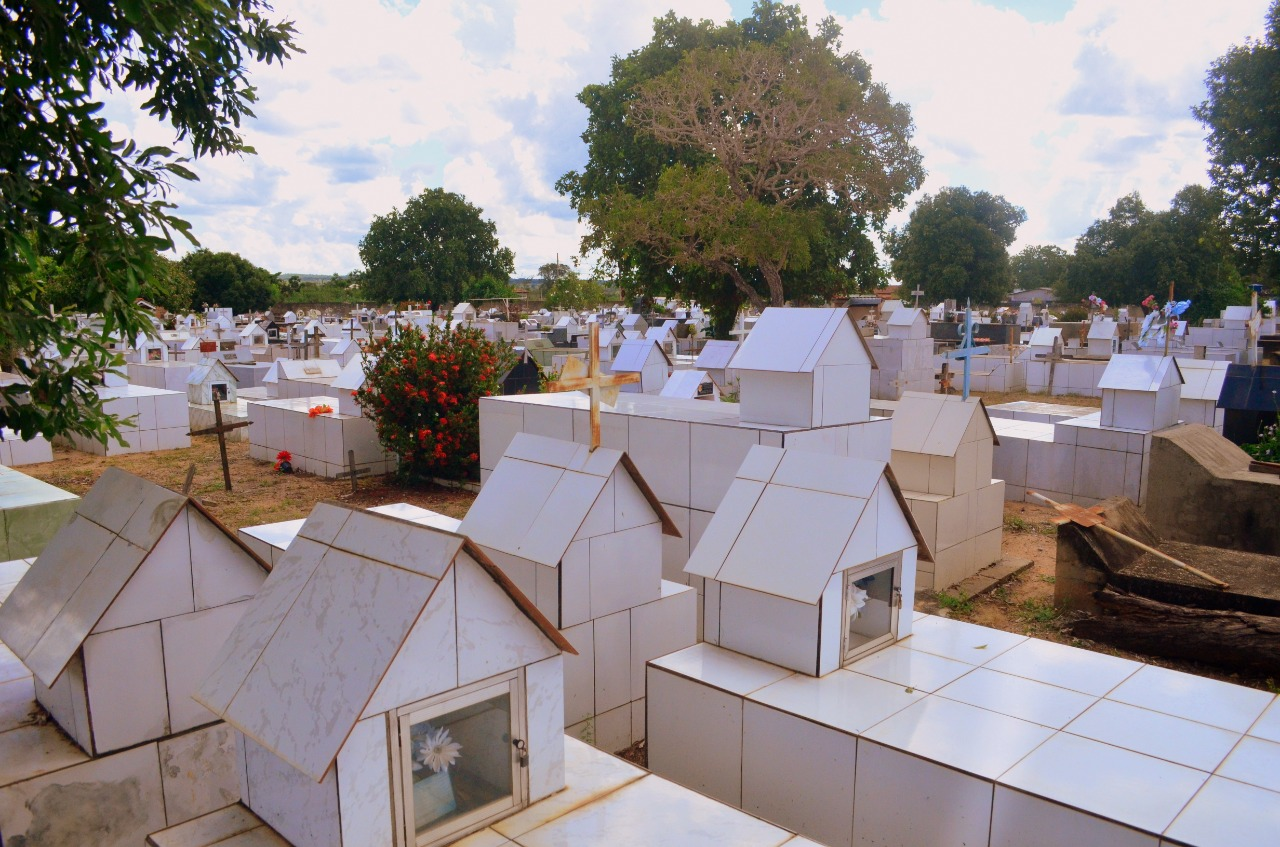
\includegraphics[width=0.5\linewidth]{802.jpeg}
    \caption{Cemitério de Barra das Graças}
    \label{fig:cemi}
\end{figure}

\subsection{Itens e Pistas}

\begin{itemize}
    \item \textbf{Peças Metálicas}: Fragmentos tecnológicos que sugerem que uma criatura alienígena passou por ali.
    \item \textbf{Pegadas com Três Dedos}: Pegadas estranhas indicam a presença de um ser não humano.
    \item \textbf{Entrada Secreta para o Intraterra}: Uma lápide afastada, que ao ser empurrada revela uma entrada para um sistema de túneis subterrâneos.
\end{itemize}

\subsection{Entrada do Intraterra}

Localizada no cemitério, leva à caverna com quatro salas e à Sala do Portal, que está trancada e deve ser monitorada.

\subsection{Cenas de Assombração no Cemitério}

O cemitério de Barra das Garças é palco de estranhas manifestações, especialmente à noite, quando figuras etéreas e sons inquietantes fazem com que poucos se atrevam a cruzar seus portões. Os fantasmas que habitam este lugar têm histórias mal resolvidas, e suas presenças perturbam a paz dos vivos. Abaixo estão três cenas de assombração, cada uma envolvendo um espírito com motivos diferentes para se manifestar.

\subsubsection{O Fantasma do Assassinado – Em Busca de Justiça}

\textbf{Cena:} Enquanto os personagens atravessam uma das alamedas do cemitério, uma figura pálida surge perto de uma lápide isolada. O espírito é de um homem jovem com roupas antigas, rasgadas e manchadas de sangue, olhando para os personagens com uma expressão de tristeza e raiva. Em uma voz baixa e trêmula, ele pede ajuda, dizendo que seu assassinato nunca foi resolvido e que o culpado continua em liberdade. O espírito se aproxima e estende a mão, indicando um lugar específico na cidade onde uma pista crucial para o caso está escondida.

O assassino do fantasma assassinado no cemitério de Barra do Garças foi \index{Bento}Bento Silva, um influente líder local com conexões obscuras. \index{Bento}Bento, conhecido por suas atividades de conspiração com os intraterrenos e pelo uso de notícias falsas para manipular a cidade, cometeu o assassinato para silenciar o fantasma, que havia descoberto sobre seus planos de exploração e aliança com forças sobrenaturais para obter controle da região. 

O fantasma, em vida, era um jornalista chamado \textbf{Joaquim Brandão}, que estava investigando as atividades ilegais de \index{Bento}Bento. Joaquim havia descoberto provas sobre as alianças perigosas que \index{Bento}Bento vinha formando e tinha intenção de publicar uma série de reportagens reveladoras. \index{Bento}Bento, temendo que as informações vazassem e afetassem sua influência, resolveu eliminar o jornalista antes que ele pudesse expor suas conexões.

Mesmo após sua morte, o espírito de Joaquim não conseguiu descansar e ficou preso ao cemitério, buscando uma forma de trazer à tona as provas que \index{Bento}Bento tentou ocultar. Essas pistas e a resolução do mistério do fantasma podem ser descobertas pelos personagens durante a investigação, fornecendo novos elementos sobre as tramas sinistras que envolvem Barra do Garças e os objetivos obscuros de \index{Bento}Bento.

\textbf{Detalhes da Assombração:}
\begin{itemize}
    \item \textbf{Manifestação Visível}: O espírito aparece claramente, mas se desvanece se os personagens se aproximam demais, obrigando-os a manter certa distância para ouvi-lo.
    \item \textbf{Voz Sussurrante}: Ele fala em sussurros, revelando fragmentos de informações sobre seu assassinato, incluindo detalhes que podem indicar o culpado.
    \item \textbf{Pistas Sobrenaturais}: Ao longo da cena, o fantasma indica pontos específicos do cemitério onde podem ser encontrados objetos enterrados ou escondidos – provas esquecidas que podem levar à resolução do caso.
\end{itemize}



\textbf{Objetivo da Cena:} Levar os personagens a investigar o local indicado pelo espírito, encontrando provas que possam ser cruciais para a resolução do crime que tirou a vida do fantasma.

\paragraph{Pistas sobre o Assassinato de Joaquim Brandão}

Durante a investigação, os personagens podem encontrar pistas deixadas pelo fantasma de Joaquim Brandão, que revelam detalhes sobre seu assassinato e a relação entre \index{Bento}Bento Silva e atividades misteriosas em Barra do Garças. Essas pistas ajudam a desvendar o mistério por trás da morte de Joaquim e fornecem evidências contra \index{Bento}Bento.

\begin{itemize}
    \item \textbf{Diário de Joaquim Brandão} - Local: Biblioteca da Cidade  
    O diário de Joaquim Brandão está guardado na seção de arquivos antigos da biblioteca da cidade. Em uma das páginas, Joaquim descreve suspeitas sobre \index{Bento}Bento Silva, mencionando “reuniões noturnas” e "alianças perigosas" que ele estava prestes a expor. A última anotação sugere que ele havia coletado provas e pretendia publicar uma reportagem reveladora.

    \item \textbf{Carta Rasgada} - Local: Escritório do Jornal  
    Nos arquivos do escritório do jornal, onde Joaquim trabalhava, os personagens encontram uma carta rasgada que menciona um “acordo com figuras ocultas” e uma “troca de informações confidenciais” entre \index{Bento}Bento e uma “força subterrânea”. A carta foi endereçada anonimamente a Joaquim, provavelmente como uma advertência para que ele abandonasse a investigação.

    \item \textbf{Relatório de Investigação Incompleto} - Local: Delegacia, Arquivos de Casos Antigos  
    Na delegacia, o escrivão Paulo Farias guardou um relatório de investigação que Joaquim havia submetido para uma possível denúncia contra \index{Bento}Bento. O documento está incompleto e foi arquivado como “pendente” devido ao desaparecimento de Joaquim. No relatório, Joaquim menciona testemunhas e cita locais específicos onde as reuniões de \index{Bento}Bento teriam ocorrido, incluindo o cemitério e um bar local.

    \item \textbf{Gravação de Voz (EVP) do Fantasma} - Local: Cemitério, próximo ao túmulo de Joaquim  
    Durante uma visita noturna ao cemitério, os personagens podem gravar uma mensagem EVP (Electronic Voice Phenomenon) do fantasma de Joaquim. Na gravação, uma voz sussurra a palavra “provas... provas no esconderijo...”. Esta pista leva os personagens a um local secreto onde Joaquim escondeu documentos que comprometeriam \index{Bento}Bento.

    \item \textbf{Fotos Reveladoras} - Local: Subsolo do Bar “Lua Cheia”  
    Joaquim escondeu um conjunto de fotos no subsolo do Bar “Lua Cheia”, onde \index{Bento}Bento realiza algumas de suas reuniões clandestinas. As fotos, tiradas discretamente por Joaquim, mostram \index{Bento}Bento em encontros suspeitos com figuras desconhecidas que têm aparência pálida e vestimentas antigas. Estas fotos são a principal prova de que \index{Bento}Bento mantinha contato direto com forças misteriosas e que eliminou Joaquim para proteger seus segredos.

    \item \textbf{Mapa de Reuniões Noturnas} - Local: Biblioteca da Cidade  
    No arquivo de mapas históricos da cidade, os personagens encontram um mapa anotado por Joaquim, com marcações em áreas onde \index{Bento}Bento e seus associados costumavam se encontrar à noite. Uma das marcações aponta para o cemitério, enquanto outras indicam pontos próximos à Serra do Roncador e ao destacamento do DTCEA-BW. Essas marcações corroboram as suspeitas de Joaquim sobre a natureza perigosa dos encontros de \index{Bento}Bento e revelam pontos estratégicos para investigação.

\end{itemize}

\paragraph{Resumo das Pistas}

Essas pistas, reunidas, revelam que Joaquim estava investigando \index{Bento}Bento Silva e possuía evidências comprometedoras sobre suas ligações com atividades ocultas e figuras misteriosas. A coleta dessas provas permite aos personagens não apenas resolverem o assassinato de Joaquim, mas também entenderem as conexões perigosas que \index{Bento}Bento mantém, levando-os a novos mistérios em Barra do Garças.



\subsubsection{O Espírito da Mãe – Preocupação pela Filha}

\textbf{Cena:} Em uma das áreas mais antigas do cemitério, os personagens sentem uma presença suave e ouvem soluços leves ao longe. Eles se deparam com o espírito de uma mulher de aparência triste e delicada, vestida com roupas antigas e segurando uma fotografia de uma menina pequena, que ela revela ser sua filha. Ela parece aflita, perguntando aos personagens se sabem onde está sua filha, pois não consegue descansar até ter certeza de que ela está bem. A mulher lamenta ter deixado a filha tão jovem e pergunta se os personagens podem verificar se sua menina está em segurança. 

\textbf{Detalhes da Assombração:}
\begin{itemize}
    \item \textbf{Aparição Melancólica}: O espírito aparece com uma expressão de tristeza e ansiedade, segurando a fotografia com delicadeza, como se fosse sua única conexão com o mundo.
    \item \textbf{Toque Gelado}: Quando ela se aproxima dos personagens, eles sentem um frio intenso, como se o desespero dela fosse palpável.
    \item \textbf{Dicas sobre a Filha}: Ao conversarem com o espírito, os personagens percebem que a menina da fotografia é agora a esposa do prefeito, uma mulher que vive em segurança, mas que nunca soube da presença da mãe. 
\end{itemize}

\textbf{Objetivo da Cena:} Dar aos personagens a oportunidade de encontrar um modo de confortar o espírito, seja comunicando-se com a filha ou levando um objeto pessoal dela para assegurar a mãe de que sua filha está em paz.

\subsubsection{O Facínora – Um Espírito Violento e Perigoso}

\textbf{Cena:} Ao se aproximarem de um mausoléu em ruínas, os personagens são subitamente atacados por pedras e pedaços de madeira que parecem ser lançados do nada. O espírito de um homem violento, conhecido em vida por seus crimes, se revela rindo e atacando os personagens sem motivo aparente. Ele tem uma aparência cruel, com um sorriso distorcido e uma postura ameaçadora, quase sólida, e arremessa objetos pesados que podem causar ferimentos graves. O facínora se alimenta do medo e só poderá ser detido por um exorcismo apropriado.

\textbf{Detalhes da Assombração:}
\begin{itemize}
    \item \textbf{Aparição Agressiva}: O espírito surge de forma sólida, tornando-se quase tangível, e tem um rosto desfigurado por uma expressão de fúria e prazer sádico.
    \item \textbf{Objetos em Movimento}: Ele arremessa objetos com uma força impressionante, criando um risco real para os personagens, que precisam se esquivar para evitar ferimentos.
    \item \textbf{Imunidade a Ataques Comuns}: Armas convencionais e tentativas de defesa física são inúteis; o facínora só pode ser repelido com rituais de exorcismo e símbolos sagrados.
\end{itemize}

\textbf{Objetivo da Cena:} Desafiar os personagens a enfrentarem o facínora com métodos sobrenaturais, como orações e símbolos sagrados, para exorcizá-lo e impedir que ele continue aterrorizando o cemitério e colocando vidas em perigo.


\subsection{NPCs}

\begin{itemize}
    \item \textbf{Sr. Carlinhos}: Gerente do Cemitério. Conhecido na cidade por saber todas as histórias do cemitério e compartilhar informações sobre atividades paranormais. Sr. Carlinhos também menciona lendas sobre uma cidade perdida nas redondezas que dizem estar conectada a espíritos obsessores, afirmando que muitas das atividades paranormais podem estar relacionadas a esses espíritos que habitam o local.
\end{itemize}




\section{Igreja de São Miguel}

A Igreja de São Miguel é uma construção imponente de estilo colonial, com uma arquitetura que remonta aos primeiros anos da cidade, carregando uma atmosfera antiga e misteriosa. Esta igreja é um ponto central para a comunidade de Barra das Garças e um local envolto em lendas e histórias sobrenaturais. 

A seguir, uma descrição detalhada dos espaços internos da igreja.

\subsection{Entrada e Foyer}

Ao adentrar a igreja pela grande porta de madeira, os visitantes se deparam com o \textbf{foyer}, um espaço de entrada amplo, com paredes adornadas por imagens religiosas e prateleiras contendo velas que os devotos acendem antes de adentrar o recinto principal. Este ambiente acolhedor introduz o visitante ao ambiente de introspecção que permeia toda a igreja.

\subsection{Nave Central e Pews}

A nave central é o coração da igreja, um longo corredor que se estende até o altar principal. O piso é feito de ladrilhos antigos que, segundo os moradores, contêm traços de mármore vindo de construções antigas. A nave é ladeada por fileiras de \textbf{bancos de madeira} escura, desgastados pelo tempo, onde os fiéis se acomodam para assistir às missas. Entre as fileiras de bancos há pequenas mesas de oração com velas acesas, que criam um ambiente místico, especialmente durante a noite.

\subsection{Capela de Oração Privada}

À esquerda da nave, uma pequena \textbf{capela de oração privada} oferece um espaço mais reservado para orações individuais. A capela é decorada com ícones religiosos menores e velas de cera pura, emitindo uma luz suave e reconfortante. Esse espaço é muitas vezes frequentado por moradores locais que buscam paz interior ou que pretendem se proteger das influências espirituais negativas que rondam a cidade.

\subsection{Sacristia}

Do lado direito da nave, uma porta discreta leva à \textbf{sacristia}, um ambiente pequeno e funcional onde são guardados objetos sagrados, como cálices, crucifixos e vestes utilizadas nas cerimônias. Há também prateleiras cheias de documentos antigos e livros religiosos que podem oferecer pistas sobre fenômenos sobrenaturais. Este espaço é considerado sagrado, e apenas o clero e assistentes podem entrar.

\subsection{Altar e Área do Santuário}

No final da nave central está o \textbf{altar principal}, uma estrutura imponente em madeira esculpida, decorada com estátuas de anjos e santos. Atrás do altar, há uma parede decorada com vitrais que representam São Miguel e outros arcanjos. Durante o dia, a luz que passa por esses vitrais ilumina o altar com um brilho colorido e intenso, dando um aspecto sobrenatural ao ambiente. No centro do altar encontra-se um grande crucifixo, ao lado de velas sempre acesas, símbolo da devoção local.

\subsection{Vitrais e Velas}

Os vitrais ao longo das paredes da igreja são um destaque à parte. Cada vitral conta uma história, desde passagens bíblicas até lendas locais, como o desaparecimento do Coronel Fawcett e as histórias dos intraterrenos. Esses vitrais coloridos permitem que a luz externa adentre o interior da igreja com um brilho difuso, criando sombras misteriosas que amplificam a atmosfera de mistério.

\subsection{Torre do Sino}

No fundo da igreja, há uma escada em espiral que leva até a \textbf{torre do sino}. Esse sino é tocado apenas em ocasiões especiais ou emergências. Da torre, é possível ter uma visão panorâmica da cidade e da Serra do Roncador ao norte. Muitos afirmam que avistamentos de luzes misteriosas no céu são frequentemente observados a partir desta torre.

\subsection{Itens e Pistas na Igreja de São Miguel}

\begin{itemize}
    \item \textbf{Vela com Brilho Azulado}: Uma vela localizada no altar que emite uma luz suave e azulada, semelhante àquela observada no cemitério. Esta vela pode ter ligação com as atividades dos intraterrenos e servir como um ponto de investigação.
    \item \textbf{Livro de Lendas Locais}: Guardado na sacristia, este livro contém relatos sobre a presença de entidades estranhas na região, incluindo espíritos obsessores e histórias sobre a cidade perdida. O livro pode fornecer informações valiosas aos agentes em busca de respostas sobre os fenômenos locais.
\end{itemize}

\subsection{Resumo}

A Igreja de São Miguel é um ponto crucial para a investigação de assombrações em Barra das Garças, proporcionando um ambiente repleto de história, religiosidade e misticismo. Com áreas reservadas e itens sagrados, a igreja serve como um local tanto de proteção quanto de mistério, onde os agentes podem encontrar pistas essenciais para resolver os enigmas que cercam a cidade.


\subsection{NPCs da Igreja de São Miguel}

Abaixo estão descritos os principais personagens que podem interagir com os agentes dentro da Igreja de São Miguel. Cada um possui um papel importante nas atividades da igreja e um histórico pessoal que adiciona profundidade à sua presença na narrativa.

\subsubsection{Sacristão Joaquim dos Santos}

\textbf{Nome:} Joaquim dos Santos  
\textbf{Idade:} 63 anos  
\textbf{Cargo:} Sacristão  
\textbf{Descrição:}  
Joaquim dos Santos é o sacristão responsável pela manutenção da Igreja de São Miguel. Um homem de baixa estatura e semblante sereno, Joaquim veste sempre roupas simples, porém bem cuidadas. Ele tem cabelos grisalhos e uma expressão de bondade, mas carrega uma aura de mistério, resultado de anos convivendo com as lendas e rumores sobrenaturais de Barra das Garças. 

Como sacristão, Joaquim organiza o altar, cuida dos objetos sagrados e prepara os itens necessários para as missas e cerimônias. Ele também se ocupa das velas e dos vitrais, sendo um dos poucos que conhece a história de cada imagem representada neles. Muitos moradores afirmam que ele já presenciou fenômenos estranhos dentro da igreja, mas Joaquim raramente fala sobre isso, a não ser que sinta que a pessoa merece ou precisa saber.

\textbf{Traços de Personalidade:}
\begin{itemize}
    \item \textbf{Sábio e Reservado}: Joaquim prefere observar e ouvir do que falar. Suas respostas são geralmente curtas, mas repletas de significados ocultos.
    \item \textbf{Conhecedor das Lendas}: Ele sabe muito sobre as lendas e mistérios da igreja e da cidade, mas escolhe cuidadosamente com quem compartilha esse conhecimento.
    \item \textbf{Protetor}: Joaquim vê a igreja como um local sagrado e está disposto a defendê-la de qualquer ameaça, incluindo fenômenos sobrenaturais.
\end{itemize}

\textbf{Habilidades e Conhecimentos Especiais:}
\begin{itemize}
    \item \textbf{Conhecimento de Rituais de Proteção}: Joaquim sabe realizar pequenos rituais de proteção e banimento, embora evite utilizá-los abertamente.
    \item \textbf{Percepção Espiritual}: Ele consegue sentir presenças espirituais na igreja e nos arredores, um dom que acredita ter herdado de sua mãe.
    \item \textbf{Artesanato Sagrado}: Joaquim possui habilidade para restaurar e proteger objetos religiosos, mantendo a sacralidade dos itens na igreja.
\end{itemize}



\subsubsection{Diácono Mateus Fontes}

\textbf{Nome:} Mateus Fontes  
\textbf{Idade:} 29 anos  
\textbf{Cargo:} Diácono  
\textbf{Descrição:}  
Mateus Fontes é o jovem diácono da Igreja de São Miguel e braço direito do Padre Anselmo. Ele é um homem alto, com cabelos castanhos e uma expressão amigável, e sua personalidade cativante faz com que seja muito querido entre os fiéis. Diácono Mateus tem uma profunda fé e acredita que sua vocação é proteger e ajudar a comunidade, especialmente diante dos eventos sobrenaturais que ocorrem em Barra das Garças.

Mateus é responsável por auxiliar nas missas, preparar os sacramentos e acompanhar Padre Anselmo nas visitas pastorais. Ele também orienta os jovens da paróquia e organiza grupos de oração para aqueles que enfrentam dificuldades espirituais. Apesar de sua juventude, Mateus é respeitado por sua sabedoria e força espiritual, e está determinado a enfrentar qualquer ameaça à segurança da igreja e da cidade.

\textbf{Traços de Personalidade:}
\begin{itemize}
    \item \textbf{Carismático e Inspirador}: Mateus sabe como motivar e acalmar as pessoas, usando sua fé para trazer esperança.
    \item \textbf{Corajoso e Altruísta}: Ele é destemido e disposto a arriscar-se para proteger sua comunidade.
    \item \textbf{Curioso sobre o Sobrenatural}: Embora seja cético quanto a algumas lendas, Mateus mantém uma mente aberta e está disposto a investigar eventos estranhos que ameacem a paz.
\end{itemize}

\textbf{Habilidades e Conhecimentos Especiais:}
\begin{itemize}
    \item \textbf{Exorcismo e Benção de Espaços}: Mateus conhece rituais de benção e tem treinamento básico em exorcismo, auxiliando Padre Anselmo quando necessário.
    \item \textbf{Conhecimento de Religião e Lendas Locais}: Ele tem um conhecimento sólido sobre teologia, mas também aprendeu lendas locais e está ciente das histórias sobre os intraterrenos.
    \item \textbf{Oratória Persuasiva}: Mateus é capaz de acalmar situações tensas e influenciar outras pessoas, um talento útil em investigações e interações comunitárias.
\end{itemize}

\subsubsection{Padre Anselmo}

\textbf{Nome:} Padre Anselmo Costa  
\textbf{Idade:} 54 anos  
\textbf{Cargo:} Pároco da Igreja de São Miguel  
\textbf{Descrição:}  
Padre Anselmo é o pároco da Igreja de São Miguel, um homem de porte austero e voz tranquila, cuja presença inspira respeito e confiança. Ele é conhecido por sua profunda devoção, sua vasta sabedoria sobre teologia e sua compreensão das histórias e lendas locais de Barra das Garças. Padre Anselmo tem cabelos grisalhos e usa sempre uma batina negra, simbolizando seu compromisso com a fé e o serviço à comunidade.

Por anos, Padre Anselmo ouviu os relatos dos moradores sobre fenômenos estranhos, incluindo visões de luzes e avistamentos de seres incomuns. Ele aconselha cautela aos seus paroquianos e evita fomentar o medo, acreditando que a paz espiritual é a melhor proteção contra influências negativas. Apesar de sua abordagem tranquila, ele leva muito a sério a presença dos chamados espíritos obsessores, que acredita serem entidades que influenciam negativamente certos moradores e eventos na cidade. Padre Anselmo compartilha esses conhecimentos apenas com aqueles que demonstram responsabilidade, incluindo agentes em missões.

\textbf{Traços de Personalidade:}
\begin{itemize}
    \item \textbf{Calmo e Reflexivo}: Padre Anselmo raramente se abala, mantendo-se sereno mesmo em situações difíceis, uma qualidade que o torna um ponto de equilíbrio para a comunidade.
    \item \textbf{Sábio e Prudente}: Ele prefere adotar uma postura de observação e reflexão, evitando confrontos diretos, especialmente com entidades que considera espiritualmente perigosas.
    \item \textbf{Empático e Protetor}: Padre Anselmo demonstra grande compaixão por sua comunidade e está sempre disposto a ajudar aqueles que buscam auxílio espiritual.
\end{itemize}

\textbf{Habilidades e Conhecimentos Especiais:}
\begin{itemize}
    \item \textbf{Conhecimento Profundo das Lendas Locais e Espirituais}: Padre Anselmo conhece em detalhes as histórias dos intraterrenos, espíritos obsessores e outros fenômenos locais, o que o torna uma fonte de informações valiosa.
    \item \textbf{Experiência em Exorcismo e Rituais de Proteção}: Ele é treinado em exorcismo e frequentemente realiza rituais de benção e proteção para moradores e para a igreja. Sua experiência é extensa, e ele sabe lidar com diferentes tipos de manifestações espirituais.
    \item \textbf{Conselheiro Espiritual}: Sua habilidade de aconselhar é acompanhada de uma capacidade de persuasão discreta e inspiradora, o que faz com que as pessoas sintam confiança em suas orientações.
\end{itemize}

\textbf{Histórico e Motivação:}  
Padre Anselmo chegou a Barra das Garças há mais de 20 anos e, desde então, testemunhou mudanças significativas na cidade. Ele acredita que algumas forças espirituais têm se intensificado nos últimos anos e que os fenômenos sobrenaturais na região podem estar ligados a atividades antigas, datando de antes mesmo da fundação da cidade. Seu papel como líder espiritual o motiva a proteger a cidade de influências negativas e a manter a paz entre os moradores. Embora seu foco seja o bem-estar da comunidade, ele entende a importância de estudar essas forças sobrenaturais para proteger melhor aqueles sob sua responsabilidade.

Essas características tornam Padre Anselmo uma figura-chave para os agentes, capaz de oferecer tanto apoio espiritual quanto informações sobre o intraterreno e outras forças misteriosas em Barra das Garças. Seu conhecimento é amplamente respeitado, e ele é um aliado confiável em missões envolvendo investigações espirituais e confrontos sobrenaturais.





\section{Irmandade de São Jerônimo}

A Irmandade de São Jerônimo é uma sociedade religiosa leiga ultraconservadora que se dedica a proteger e preservar os valores e a tradição religiosa da cidade de Barra das Garças. A irmandade foi fundada há várias décadas por imigrantes italianos, e seus membros são conhecidos por sua rigidez em relação aos costumes e moralidade. Eles exercem grande influência na comunidade, inclusive na política local, tendo entre seus membros o vereador Alceu Braga, que utiliza seu cargo para promover as pautas da irmandade.

\subsection{O Prédio da Irmandade}

O edifício da Irmandade de São Jerônimo é um prédio antigo de dois andares, com uma arquitetura que remonta ao período colonial, construído com pedras rústicas e janelas de madeira trabalhada. No interior, o ambiente é austero e decorado com imagens sacras, cruzes e velas que iluminam discretamente os corredores e salas. Em uma das salas, protegida por uma porta de madeira maciça e um cadeado antigo, está a sala de relíquias e registros da irmandade, onde documentos secretos são guardados. A irmandade mantém registros de eventos e atividades de grupos considerados perigosos por eles, além de objetos religiosos que possuem um significado simbólico e espiritual.

A sala de reuniões da irmandade contém uma grande mesa de madeira onde os membros discutem e decidem os rumos da organização. Uma das paredes abriga uma cruz de ferro antiga, que, segundo a tradição, teria sido abençoada por um sacerdote exorcista e utilizada em um ritual de expulsão de espíritos.

\subsection{Personagens da Irmandade}

\paragraph{Vereador Alceu Braga}  
O vereador Alceu é um homem na casa dos 50 anos, com uma postura rígida e conservadora. Alceu é influente na comunidade e utiliza seu cargo para impulsionar projetos de lei que reforçam os valores da irmandade. Ele é visto com desconfiança por grupos religiosos afrodescendentes e figuras políticas progressistas da cidade.

\paragraph{Ancião Giovanni Borelli}  
Com 82 anos, Giovanni é o membro mais antigo e respeitado da irmandade. Ele herdou uma relíquia dos pais, imigrantes italianos que trouxeram um crucifixo de prata, supostamente com poderes de exorcismo. Giovanni é discreto e raramente fala sobre a relíquia, mas é o único que sabe como utilizá-la em rituais de banimento de espíritos. Acredita-se que o crucifixo tenha sido usado em um evento de exorcismo ainda na Itália e, desde então, permaneceu na família.

\paragraph{Padre Júlio, o Conselheiro}  
Padre Júlio, de 64 anos, não é um membro oficial da irmandade, mas participa das reuniões como conselheiro espiritual. Ele é muito respeitado e orienta os membros sobre práticas religiosas. Padre Júlio preza pelo segredo das atividades da irmandade e insiste que os registros de rituais permaneçam sigilosos.

\paragraph{Marco Pereira, o Guardião}  
Marco, de 43 anos, é o responsável pela segurança do prédio da irmandade. Ele garante que ninguém entre nas áreas restritas sem permissão. Marco é um homem discreto, de poucas palavras, e possui um treinamento em autodefesa. Ele guarda a sala de relíquias com grande dedicação e possui um rosário que, segundo ele, protege contra influências malignas.

\paragraph{Ricardo Oliveira, o Escriturário}  
Ricardo é um homem meticuloso, responsável pela manutenção dos arquivos da irmandade. Aos 37 anos, ele mantém uma postura rígida e é extremamente zeloso com os documentos da organização. Ricardo possui um caderno secreto onde registra detalhes de todas as reuniões, mas mantém o conteúdo em segredo até mesmo para seus colegas.

\paragraph{Lucas Mendes, o Noviço}  
Lucas é o membro mais jovem da irmandade, com 24 anos. Ele foi iniciado recentemente e está aprendendo os segredos da organização. Lucas tem uma admiração por Giovanni e deseja aprender sobre o uso da relíquia, mas Giovanni reluta em revelar o segredo do crucifixo.

\section{Religiões Afrodescendentes em Barra das Garças}

Em Barra das Garças, as religiões afro-brasileiras têm uma presença significativa, com três terreiros que acolhem uma parte importante da comunidade. O mais influente deles é o Terreiro de Pai Jorge, conhecido por realizar rituais e cerimônias que atraem fiéis e curiosos da região.

\subsection{Terreiro de Pai Jorge}

O Terreiro de Pai Jorge é o maior e mais respeitado da cidade, fundado por Jorge de Xangô, um sacerdote conhecido por seu conhecimento profundo da Umbanda e do Candomblé. O terreiro é um espaço amplo, cercado por plantas sagradas e decorado com estátuas e elementos que representam os orixás. Pai Jorge é conhecido por seus rituais poderosos e por sua sabedoria espiritual, além de ser guardião de alguns segredos espirituais importantes para a comunidade.

\paragraph{Pai Jorge de Xangô}  
Líder espiritual do terreiro, Pai Jorge, de 58 anos, é um respeitado sacerdote com habilidades reais em magia branca. Ele possui uma forte conexão com o orixá Xangô e é capaz de realizar rituais de proteção e cura que possuem efeitos notáveis. Pai Jorge é o conselheiro de muitos moradores e mantém um bastão sagrado, utilizado em rituais específicos de benção e purificação.

\paragraph{Mãe Cleonice, a Curandeira}  
Mãe Cleonice, de 62 anos, é uma mulher de grande conhecimento herbal e ajuda a comunidade com ervas e poções de cura. Ela é responsável pela preparação dos banhos e infusões que ajudam nas práticas espirituais do terreiro. Cleonice guarda consigo um amuleto abençoado pelo orixá Oxum, que dizem trazer sorte e prosperidade para quem o possui.

\paragraph{Joaquim, o Ogã}  
Joaquim é o ogã do terreiro, responsável pela música e pelos cânticos sagrados durante as cerimônias. Aos 45 anos, Joaquim é hábil no uso do atabaque e possui um colar que representa a proteção do orixá Ogum. Ele é considerado um defensor espiritual do terreiro e está sempre presente para apoiar os rituais de Pai Jorge.

\paragraph{Luciana, a Filha de Santo}  
Com 30 anos, Luciana é uma filha de santo de Pai Jorge, devota de Iemanjá. Ela participa dos rituais de purificação e proteção e auxilia nas cerimônias. Luciana possui um espelho sagrado, presente de Mãe Cleonice, que utiliza em rituais de meditação e fortalecimento espiritual.

\paragraph{Terreiros Menores}

Além do Terreiro de Pai Jorge, há outros dois terreiros em Barra das Garças:

\subsubsection{Terreiro de Mãe Celina}  
Um terreiro menor, mas ativo, liderado por Mãe Celina, que realiza rituais de purificação e consultas espirituais.

\subsubsection{Terreiro de Pai Ernesto}  
Conhecido por seus rituais noturnos, Pai Ernesto é um sacerdote que ajuda os moradores a resolver problemas pessoais e espirituais por meio das práticas religiosas afro-brasileiras.

\section{Outras Igrejas de Barra das Garças}

Além da Igreja de São Miguel, existem outras duas pequenas igrejas na cidade, cada uma com suas particularidades e liderança.

\subsection{Igreja de Santa Clara}

A Igreja de Santa Clara é uma pequena capela localizada no bairro mais antigo da cidade. É uma construção modesta, mas frequentada por uma comunidade fiel.

\paragraph{Padre Carlos}  
O responsável pela Igreja de Santa Clara, Padre Carlos, é um homem de 55 anos, com uma abordagem acolhedora e humilde. Ele é conhecido por sua proximidade com a comunidade e por oferecer apoio espiritual para todos os que procuram a igreja. Padre Carlos possui um crucifixo de prata que foi presente de sua avó e acredita que o objeto é abençoado.

\paragraph{Sacristão Antônio}  
Antônio é o sacristão de 46 anos que cuida da igreja com zelo. Ele é tímido e reservado, mas extremamente devoto e leal a Padre Carlos. Antônio guarda um pequeno relicário de Santa Clara, que ele afirma proteger a igreja de más influências.

\subsection{Capela de Nossa Senhora das Dores}

A Capela de Nossa Senhora das Dores é um templo discreto e pacífico, cercado por um jardim bem cuidado. A capela é administrada por Padre Francisco, que realiza missas semanais e acolhe fiéis de toda a cidade.

\paragraph{Padre Francisco}  
Padre Francisco, de 60 anos, é um religioso experiente, com uma postura serena e compassiva. Ele dedica-se à orientação espiritual dos fiéis e realiza visitas constantes às famílias da região. O padre possui um rosário que, segundo ele, já foi utilizado em uma bênção especial, o que lhe confere uma energia protetora.

\paragraph{Sacristão Paulo}  
Paulo é um jovem de 28 anos que auxilia Padre Francisco nas atividades da capela. Ele é conhecido por sua devoção e entusiasmo. Paulo possui um livro antigo de orações, passado de geração em geração em sua família


\section{Comunidades Evangélicas em Barra das Garças}

Em Barra das Garças, as comunidades evangélicas são diversas e incluem várias denominações com templos espalhados por toda a cidade. Cada corrente possui suas próprias doutrinas e modos de adoração, refletindo a diversidade de interpretações e práticas dentro do protestantismo. Abaixo, descrevemos quatro correntes evangélicas representativas na cidade, cada uma com seus templos e líderes.

\subsection{Igreja do Caminho da Fé}

A Igreja do Caminho da Fé é uma das congregações evangélicas mais tradicionais da cidade, com uma doutrina voltada para o estudo bíblico e a promoção de valores familiares. O templo principal é grande e possui um auditório com capacidade para centenas de pessoas, decorado de maneira simples e funcional, com ênfase na palavra e na comunhão.

\paragraph{Pastor Eduardo Reis}  
Pastor Eduardo é um líder respeitado, com um forte compromisso com a comunidade e um estilo de vida modesto. Ele é conhecido por suas pregações baseadas na caridade e na justiça social, realizando projetos de assistência para os necessitados da cidade. Eduardo promove cursos de formação bíblica e incentiva a participação dos jovens na igreja, buscando construir uma comunidade unida e altruísta. Sua abordagem caridosa e sincera faz dele uma figura admirada até mesmo fora do meio evangélico.

\subsection{Comunidade Esperança Celestial}

A Comunidade Esperança Celestial é uma igreja pentecostal que valoriza o louvor e a experiência espiritual intensa em suas celebrações. Seus cultos incluem cânticos animados, orações em grupo e eventos de evangelização. O templo é decorado com cores vivas e possui uma grande cruz iluminada no altar, sendo o principal ponto de encontro da comunidade para cultos semanais e eventos especiais.

\paragraph{Pastor Miguel Rocha}  
Pastor Miguel é um líder carismático e reconhecido por suas habilidades de comunicação. Sua pregação é enérgica, e ele é conhecido por enfatizar a importância da fé para a conquista de milagres e bênçãos na vida pessoal e familiar de seus fiéis. Embora seja visto como um pastor “normal”, Pastor Miguel é cuidadoso em suas ações e não se envolve em polêmicas, mantendo um bom relacionamento com os fiéis e com as outras lideranças religiosas da cidade.

\subsection{Templo da Prosperidade Divina}

O Templo da Prosperidade Divina é uma congregação de doutrina neopentecostal, focada em temas de prosperidade financeira e “batalha espiritual”. O templo é grandioso, com equipamentos de som e luz modernos, e ostenta uma fachada imponente que chama atenção. Os cultos enfatizam o poder da doação para a obtenção de bênçãos e prosperidade.

\paragraph{Pastor Osvaldo Santos}  
Pastor Osvaldo é uma figura polêmica na cidade, frequentemente criticado por sua insistência em campanhas de doação de altos valores e promessas de retorno financeiro divino para os fiéis. Ele vive de forma ostensiva, com roupas e acessórios de luxo, o que levanta suspeitas entre a população sobre a real destinação das doações. Muitos acreditam que Pastor Osvaldo explora a fé dos fiéis, e há rumores de que ele está envolvido em esquemas financeiros. Apesar das críticas, ele mantém uma base fiel de seguidores e justifica seu estilo de vida como resultado das “bênçãos de Deus”.

\subsection{Igreja Batista do Vale}

A Igreja Batista do Vale é uma congregação discreta e acolhedora, com um estilo de adoração mais tranquilo e um forte foco em projetos sociais. O templo é simples, mas bem cuidado, com uma pequena biblioteca e um espaço para atividades de estudo bíblico e recreação para crianças e jovens. A igreja é conhecida por suas campanhas de ajuda aos mais necessitados e seu envolvimento em atividades de responsabilidade social.

\paragraph{Pastor Roberto Silva}  
Pastor Roberto é um homem dedicado e responsável, que guia a igreja de maneira serena e comedida. Ele é um líder respeitado, embora mantenha um perfil discreto e reservado. Pastor Roberto se dedica ao estudo bíblico e incentiva os fiéis a buscar uma vida de retidão e serviço à comunidade. Ele promove cursos de formação cristã e programas de apoio à juventude. Como líder, Pastor Roberto é visto como “normal”, uma presença constante e confiável para a comunidade batista do bairro.

\subsection{Visão Geral das Correntes Evangélicas}

Cada uma dessas comunidades representa um segmento da diversidade evangélica na cidade, com abordagens distintas em relação à fé e à forma de conduzir o templo. Enquanto a Igreja do Caminho da Fé se destaca pelo compromisso social de Pastor Eduardo, a Comunidade Esperança Celestial é um centro de adoração vibrante e acolhedor. Em contraste, o Templo da Prosperidade Divina levanta questões de ética e sinceridade nas práticas de Pastor Osvaldo, atraindo tanto fiéis quanto críticas pela ênfase em doações. Já a Igreja Batista do Vale destaca-se pelo trabalho comunitário, uma característica prezada por Pastor Roberto e seus seguidores.

Essas diferenças refletem as várias facetas das comunidades evangélicas em Barra das Garças, que coexistem apesar de suas diferenças, oferecendo opções distintas de adoração e práticas religiosas para a população local.

\section{O Coven de Ágata Negra e Suas Bruxas}

Escondido nos limites de Barra das Garças, o Coven de Ágata Negra é um círculo de bruxas conhecidas por práticas esotéricas e conhecimentos antigos. Elas se reúnem em uma clareira na floresta, em noites de lua cheia, para rituais que conectam suas forças à natureza e aos elementos. O coven é formado por cinco bruxas, cada uma com habilidades únicas, que, unidas, criam uma forte presença mística na região.

\subsection{A Sede do Coven}

A sede do coven, conhecida como ``Casa de Ágata Negra'', é uma cabana rústica e oculta, cercada por árvores antigas e flora densa. Com velas e amuletos pendurados nas janelas, a casa parece distante da cidade, tanto física quanto espiritualmente. Dentro, o ambiente é decorado com objetos ritualísticos: cristais, ervas secas e livros de feitiçaria. Um altar no centro da sala é dedicado à deusa da natureza, com oferendas de flores, frutas e pequenos animais esculpidos em madeira.

\subsection{As Bruxas do Coven}

\paragraph{Helena, a Matriarca}  
Helena é a bruxa mais velha e respeitada do coven, conhecida como a matriarca. Ela possui vasto conhecimento sobre plantas medicinais e poções curativas. Helena também é guardiã de um grimório ancestral, passado de geração em geração, que contém feitiços poderosos de proteção e cura. Sua presença imponente inspira confiança e respeito entre as outras bruxas.

\paragraph{Mara, a Visionária}  
Mara é uma jovem bruxa com habilidades visionárias, capaz de realizar premonições e leituras de cartas com impressionante precisão. Seu poder intuitivo lhe permite prever acontecimentos futuros, e ela frequentemente guia o coven sobre decisões importantes. Embora seja reservada, sua sabedoria mística é valiosa para o grupo.

\paragraph{Selena, a Guardiã dos Espíritos}  
Selena é uma bruxa de meia-idade com habilidades de comunicação com espíritos. Ela serve como mediadora entre o mundo dos vivos e o dos mortos, realizando rituais de proteção e purificação. Selena é conhecida por seus amuletos protetores e práticas de exorcismo, sendo procurada por pessoas que acreditam estar sendo assombradas.

\paragraph{Bianca, a Feiticeira Elemental}  
Bianca é uma bruxa hábil em manipular os elementos, especialmente a água e o fogo. Seus feitiços são conhecidos por sua intensidade e precisão. Bianca é responsável pelos rituais ligados à natureza e à renovação, sendo uma figura essencial durante as celebrações de solstícios e equinócios. Ela possui um bastão encantado que utiliza para canalizar sua energia elemental.

\paragraph{Isabel, a Aprendiz}  
Isabel é a mais nova do grupo e aprendiz do coven. Embora inexperiente, ela demonstra grande aptidão para feitiços de cura e proteção. Isabel está sob a orientação direta de Helena, aprendendo as tradições e práticas da magia ancestral. Sua curiosidade e determinação a tornam uma promessa para o futuro do coven.

\subsection{Segredos e Rituais}

O coven guarda alguns segredos que são conhecidos apenas por suas integrantes. Um desses segredos envolve a ``Relíquia de Ágata'', uma pedra negra com propriedades místicas, que dizem ser a chave para aumentar os poderes de cura de quem a possui. Helena é a guardiã dessa relíquia e utiliza-a em ocasiões especiais para fortalecer os rituais de proteção.

Outro segredo é o ``Feitiço da Nuvem Sombria'', um ritual poderoso que o coven utiliza em casos de extrema necessidade para proteger a comunidade de forças negativas. Esse feitiço é raro e demanda grande energia das bruxas, sendo reservado apenas para momentos críticos.

\subsection{Rituais e Festividades}

O coven celebra regularmente as mudanças de estação e as fases da lua, com destaque para os solstícios e equinócios. Esses eventos são oportunidades de renovação espiritual, nos quais as bruxas realizam rituais para agradecer à natureza e reforçar seus laços com o ambiente. As festividades são momentos de união, onde cada bruxa contribui com seu dom único, fortalecendo os laços do grupo e renovando o poder coletivo do coven.

Com o tempo, o Coven de Ágata Negra tem se tornado uma lenda em Barra das Garças, uma presença oculta e poderosa, cercada por mistérios e reverência. Suas bruxas, com habilidades distintas e complementares, formam um grupo que preserva o conhecimento ancestral, transmitindo-o de geração em geração e protegendo a comunidade dos perigos invisíveis do mundo místico.


\chapter{Locais Místicos}

Este capítulo apresenta uma descrição dos principais locais místicos da cidade, onde o sobrenatural se mistura com o cotidiano, criando uma atmosfera de mistério e fascinação. Esses locais abrigam personagens e fenômenos enigmáticos que contribuem para o misticismo e as lendas urbanas do lugar.

\section{Oráculo Local}
Um dos pontos mais enigmáticos da cidade é a cabana do Oráculo, um(a) ancião(ã) que vive em isolamento em uma floresta densa nos arredores da cidade. Esse(a) personagem possui a habilidade de prever o futuro e é procurado(a) tanto por pessoas comuns quanto por figuras influentes em busca de orientação. Embora seja conhecido(a) por suas previsões, o Oráculo esconde segredos profundos sobre suas origens e a natureza real dos seus poderes, que podem estar ligados a forças de outras dimensões ou a um pacto com entidades ancestrais.

\dperson{Oráculo, ancião da floresta}{
O Oráculo é um(a) ancião(ã) que vive isolado(a) em uma floresta densa nos arredores da cidade. Esse(a) personagem possui habilidades proféticas e é procurado(a) tanto por pessoas comuns quanto por figuras influentes em busca de orientação. Suas origens e a natureza de seus poderes são envoltas em mistério, e há rumores de que suas previsões possam estar ligadas a forças de outras dimensões ou pactos com entidades ancestrais.}{}


\section{Mercado Místico}

O Mercado Místico é um ponto central na vida sobrenatural da cidade, um evento itinerante que surge misteriosamente em diferentes locais, sempre às vésperas de eventos cósmicos ou lunares. Com um visual caótico e envolvente, as barracas são dispostas de forma aparentemente aleatória, adornadas com luzes de velas, tecidos antigos e símbolos arcanos. O mercado atrai um público diversificado, desde curiosos até praticantes das artes místicas, todos em busca de itens raros e poderes ocultos. Cada barraca parece ter uma aura própria, e os donos são personagens únicos que inspiram tanto fascinação quanto desconfiança.

\subsection{Barracas e seus Donos}

\subsubsection{A Barraca de Amuletos de Ciro}
Ciro é um ancião misterioso, conhecido por seu vasto conhecimento em simbologia e proteção espiritual. Sua barraca é repleta de amuletos de todas as partes do mundo: talismãs egípcios, pentagramas de ferro, olhos turcos, e peças encantadas por xamãs do norte da Europa. Ciro diz que cada amuleto é infundido com uma energia específica, escolhendo seu portador. Ele também oferece um ritual especial para ativar os amuletos e maximizar sua proteção, um processo que, segundo ele, envolve uma conexão direta com a "essência astral" do comprador. Rumores dizem que Ciro possui um amuleto de poder supremo escondido em sua barraca, e que ele só o vende para aqueles que enfrentam perigos sobrenaturais iminentes.


\dperson{Ciro, ancião especialista em amuletos}{ 
Ciro é um homem de aparência envelhecida, com olhos profundos e penetrantes, vestindo roupas simples adornadas com símbolos místicos discretos que, para ele, têm significados específicos. Ele é reservado, cauteloso e fala pausadamente, escolhendo as palavras com cuidado enquanto observa atentamente as intenções dos outros. Embora bem-humorado em ocasiões, ele mantém distância emocional, tratando cada pessoa como uma combinação única de energias. Ciro guarda segredos profundos sobre amuletos, conhecendo materiais e rituais que amplificam ou protegem energias espirituais. Há rumores de que ele possui um amuleto de proteção suprema, revelado apenas a poucos, que se conecta diretamente com a essência astral do portador. Ele também detém o conhecimento de um ritual que "desperta" amuletos, transformando-os em protetores espirituais conscientes, um segredo perigoso passado apenas a iniciados. Ciro é visto como um protetor da cidade, equilibrando as forças invisíveis e aconselhando quem considera necessário sobre perigos místicos, embora nunca revele as fontes de seu conhecimento.}{} 

\subsubsection{A Tenda das Poções de Yolanda}
Yolanda, uma mulher de presença intensa e voz rouca, possui uma tenda aromática com frascos de todos os tamanhos, cores e ingredientes exóticos. Ela é uma alquimista famosa por suas poções, que variam desde elixires de cura até compostos para manipulação mental e atração amorosa. Cada poção é preparada com ingredientes secretos que ela obtém em viagens misteriosas, e alguns dizem que ela possui acesso a portais para outras dimensões, onde coleta ingredientes místicos. Yolanda também é conhecida por uma poção específica, o “Soro da Verdade Oculta”, uma substância raríssima que permite ao consumidor enxergar a verdadeira essência das pessoas e de si mesmo. No entanto, ela alerta que essa poção traz consequências inesperadas para aqueles que não estão prontos para confrontar suas próprias verdades.

\dperson{Yolanda, alquimista de poções}{
Yolanda é uma mulher de presença intensa e voz rouca, conhecida por seu conhecimento em alquimia e pela criação de poções que vão desde elixires de cura até compostos para manipulação mental e atração amorosa. Suas poções são preparadas com ingredientes secretos, adquiridos em locais místicos, e ela é especialmente conhecida pelo “Soro da Verdade Oculta,” um elixir raro que permite ao consumidor enxergar a verdadeira essência das pessoas, mas com consequências imprevisíveis para os despreparados. Yolanda guarda segredos sobre portais para outras dimensões, onde, segundo dizem, coleta alguns de seus ingredientes mais poderosos.}{}


\subsubsection{A Barraca de Relíquias Antigas de Vincenzo}
Vincenzo é um colecionador de relíquias que afirma ser descendente direto de uma antiga linhagem de bruxos italianos. Sua barraca é uma das mais impressionantes do mercado, decorada com veludo vermelho e madeira entalhada, e exibe itens que parecem ter centenas de anos. Entre os objetos estão anéis, espelhos mágicos, estatuetas de divindades esquecidas e ossos encantados. Vincenzo sempre conta uma história intrigante sobre cada peça e é famoso por seu amuleto especial, um anel que dizem ter o poder de amplificar as habilidades sobrenaturais de quem o usa. Há rumores de que Vincenzo possui um diário oculto, supostamente escrito por seu antepassado, que contém segredos sobre feitiços e rituais proibidos.

\dperson{Vincenzo, colecionador de relíquias e cigano italiano}{
Vincenzo é um cigano italiano de personalidade magnética, conhecido por sua habilidade de conversar em várias línguas, um talento que ele usa para negociar e contar histórias de suas relíquias. Sua barraca no mercado místico é um espetáculo à parte, decorada com tecidos vibrantes e objetos antigos que parecem carregar uma energia própria. Vincenzo afirma ser descendente de uma linhagem de bruxos italianos, e cada peça em sua coleção é acompanhada de uma narrativa envolvente, muitas vezes contada em italiano, espanhol, ou até latim. Ele guarda relíquias raras, como um anel especial que dizem amplificar habilidades sobrenaturais. Vincenzo é tanto um comerciante astuto quanto um protetor de antigos segredos, mantendo um diário oculto que, segundo rumores, contém feitiços e rituais proibidos de sua ancestralidade.}{}




\subsubsection{A Tenda dos Sonhos de Ezra}

Ezra é um homem jovem e excêntrico, cuja especialidade é a manipulação de sonhos. Em sua tenda, ele oferece “essências dos sonhos”, frascos de cristais líquidos que prometem proporcionar sonhos lúcidos, curar traumas subconscientes e até induzir visões proféticas. Ele coleta essas essências de templos antigos e locais de poder ao redor do mundo. Ezra também oferece sessões de "guias de sonhos", onde ele promete ajudar o cliente a interpretar símbolos ocultos de suas experiências oníricas e desbloquear potencialidades ocultas. Ezra afirma que os sonhos são a ponte mais próxima entre os mortais e o sobrenatural e que, ao atravessá-los, é possível conversar com os espíritos dos ancestrais.

Na verdade, Ezra é um traficante de drogas, podendo se comprar tudo dele, porém ele é muito discreto e não vende para estranhos, precisa confiar na pessoa. Tem clientes constantes, inclusive algumas pessoas famosas na cidade, como a esposa do prefeito.


\dperson{Ezra, manipulador de sonhos e traficante discreto}{
Ezra é um jovem de aparência intrigante, com cabelos escuros e despenteados, olhos penetrantes e inquietos, sempre atentos ao ambiente ao seu redor. Ele possui uma constituição magra, mas sua presença é envolvente, quase hipnótica, reforçada por roupas que misturam o estilo boêmio e o excêntrico. Ezra costuma usar colares e anéis com pedras que ele diz “amplificar as energias dos sonhos,” mas que muitos suspeitam serem mais uma parte de seu personagem místico.\newline
No trato com as pessoas, Ezra é atencioso e, ao mesmo tempo, reservado; ele raramente fala mais do que o necessário, preferindo observar e deixar que os outros revelem suas intenções primeiro. Com os clientes, é sempre educado e gentil, mas mantém uma distância emocional que transmite tanto respeito quanto cautela. Ezra só mostra seu lado mais agressivo com aqueles que ameaçam sua confiança ou quebram seus acordos, sendo conhecido por lidar duramente com clientes inadimplentes ou traiçoeiros, mas nunca de forma impulsiva ou indiscriminada. Para aqueles em quem confia, ele é leal e confiável, oferecendo seus produtos e conselhos com uma rara atenção aos detalhes.}{}






\section{Biblioteca Oculta}
Escondida nas profundezas de um edifício antigo ou talvez abaixo da catedral, encontra-se a Biblioteca Oculta. Esse local guarda grimórios proibidos, documentos de eventos sobrenaturais e livros de história mística. O bibliotecário, uma figura reclusa e enigmática, parece não envelhecer e conhece cada lenda e mistério da cidade. A biblioteca é acessível apenas por aqueles que possuem uma permissão especial, e muitos acreditam que ela guarda segredos que poderiam mudar o destino da cidade, incluindo antigos rituais e artefatos de grande poder.


A Biblioteca Oculta é um verdadeiro santuário de conhecimentos proibidos, escondido nas profundezas de um edifício histórico da cidade. Poucos têm acesso a esse espaço, e seu conteúdo é protegido por encantamentos e barreiras mágicas. O guardião da biblioteca, conhecido apenas como Sebastian, é uma figura imponente e reclusa. Ele parece não envelhecer e demonstra um conhecimento enciclopédico sobre o mundo místico. Diz-se que Sebastian tem habilidades de telepatia, o que lhe permite saber instantaneamente as intenções de qualquer visitante, mas é apenas sua experiência.

\dperson{Sebastian, guardião da Biblioteca Oculta}{
Sebastian é um homem de aparência severa e enigmática, com pele pálida e traços que parecem eternamente jovens, o que alimenta rumores sobre sua verdadeira idade. Ele é alto e esguio, sempre vestido em roupas escuras e elegantes, incluindo um manto longo que arrasta suavemente ao caminhar. Seus olhos são intensos, quase hipnotizantes, e raramente piscam, o que dá a impressão de que ele pode ver além das aparências. \newline
No trato com os visitantes da Biblioteca Oculta, Sebastian é formal e quase intimidador. Ele fala de maneira calma e medida, escolhendo palavras como se cada uma carregasse um peso específico. Para aqueles que vêm em busca de conhecimento sincero, ele é um guia atento e até gentil, compartilhando fragmentos de sabedoria. No entanto, é inflexível com aqueles que demonstram arrogância ou ambição egoísta, muitas vezes desestimulando suas buscas com respostas enigmáticas ou, em casos extremos, negando acesso aos livros mais perigosos. Dizem que Sebastian possui habilidades telepáticas e é capaz de sentir as intenções de quem entra na biblioteca, tornando-se um guardião eficaz contra qualquer ameaça ao acervo místico, mas não é verdade. Ele apenas é experiente.}{}



\subsection{Livros e Manuscritos}

\subsubsection{O Codex Maleficarum}
Este grimório antigo é escrito em uma linguagem arcana que poucos conseguem decifrar. O Codex Maleficarum contém instruções detalhadas sobre invocações de entidades e pactos. Cada seção do livro possui símbolos místicos que parecem mudar de posição, revelando e escondendo segredos conforme a pessoa tenta ler. Sebastian alerta que este livro é perigoso e que só os praticantes mais experientes podem consultá-lo sem consequências espirituais desastrosas. Rumores dizem que o livro tem vida própria e escolhe as pessoas dignas de seu conhecimento.

\subsubsection{O Manuscrito da Lua Sanguínea}
Um dos volumes mais procurados na biblioteca é o Manuscrito da Lua Sanguínea, um livro raro que aborda rituais de cura e proteção que devem ser realizados em noites de lua cheia. Escrito por um alquimista do século XVII, o livro detalha as influências dos ciclos lunares no corpo e na alma. Ele inclui diagramas de círculos de proteção e feitiços que supostamente reforçam a conexão entre o ser humano e o poder místico da lua. A lenda local diz que este manuscrito foi usado para proteger a cidade de uma entidade sombria no passado.

\subsubsection{A Coletânea dos Oráculos}
Este é um conjunto de pergaminhos e papiros escritos por diversos videntes ao longo dos séculos, contendo profecias que já se realizaram e outras que ainda permanecem um mistério. Sebastian permite que apenas poucos leiam a Coletânea, pois acredita-se que as profecias podem ser interpretadas de várias formas, e um olhar errado pode desencadear eventos indesejados. Esse conjunto é especialmente popular entre políticos e líderes que desejam obter vantagens em suas decisões, mas é sempre alertado que nem todas as previsões são positivas.

\subsubsection{O Livro dos Espíritos Ancestrais}
Esse livro é um guia detalhado sobre como invocar e comunicar-se com espíritos de linhagens passadas. Ele contém rituais que variam de simples conexões com ancestrais até pactos com espíritos de antigos guerreiros. Para Sebastian, esse é um dos livros mais respeitados da biblioteca, pois permite o contato com aqueles que moldaram o passado da cidade e pode revelar segredos esquecidos de tempos remotos. Contudo, ele alerta que o Livro dos Espíritos Ancestrais possui riscos profundos, pois alguns espíritos são manipuladores e tentam permanecer no plano terreno a qualquer custo.


\section{Cabana do Curandeiro (ou Alquimista)}
Nas margens da cidade, existe uma cabana onde vive um(a) curandeiro(a) ou alquimista. Esse(a) personagem é conhecido(a) por suas habilidades em criar elixires, poções curativas e amuletos de proteção. Em seu laboratório, repleto de frascos e ervas secas, ele(a) prepara misturas misteriosas para os que buscam cura ou auxílio espiritual. A cabana é também um local de aprendizado sobre as plantas e seus poderes. Um segredo envolve o(a) curandeiro(a), que usa ingredientes raros e perigosos para suas poções, mantendo habilidades e um conhecimento que poucos possuem.

\dperson{Curandeiro, sábio das ervas}{
O Curandeiro é um homem de aparência desgastada, com cabelos grisalhos e mãos marcadas pelo tempo e trabalho com ervas e raízes. Suas roupas são simples e tingidas com manchas de plantas. Ele age de forma tranquila e atenciosa, falando pouco e observando muito, transmitindo uma sensação de calma e profundidade. Sua presença é acolhedora, mas há uma seriedade em seu olhar, como se carregasse segredos antigos e sagrados.}{}



\section{Entidade Protetora da Cidade}
Uma antiga entidade é reverenciada como protetora da cidade, manifestando-se em momentos críticos como uma sombra, um corvo ou uma presença sutil no vento. Habitantes realizam rituais e oferendas para essa entidade, acreditando que ela traz proteção e harmonia. Sua origem é desconhecida, mas existem histórias que dizem que essa entidade possui um vínculo com os primeiros habitantes da região, selado por um pacto. Apesar de sua natureza benevolente, há mistérios sobre a verdadeira intenção dessa entidade e seu poder oculto sobre a cidade.

\section{Sociedade Secreta}
A cidade abriga uma sociedade secreta formada por estudiosos e ocultistas que dedicam suas vidas a entender e controlar os fenômenos sobrenaturais do local. Seus membros incluem líderes religiosos, políticos e acadêmicos, cada um com um objetivo oculto. A sociedade possui um acervo de documentos e artefatos antigos, e seu conhecimento sobre a cidade é vasto. Alguns rumores dizem que o grupo planeja manipular as forças místicas para benefício próprio, enquanto outros acreditam que buscam proteger a cidade de uma ameaça sobrenatural iminente.

\section{Folclore Local}
Os habitantes da cidade compartilham uma rica tradição de lendas urbanas, contos sobre criaturas e fenômenos inexplicáveis. Há histórias sobre uma ``hora fantasma'' em que a cidade é coberta por uma névoa sobrenatural, bem como lendas sobre um lago onde espíritos aparecem em noites de lua cheia. Esses contos são passados de geração em geração, criando uma atmosfera mística e reforçando o temor e o respeito pelo desconhecido.

\section{Templo Esquecido}
Nas montanhas ou em uma floresta afastada, existe um templo em ruínas, considerado sagrado por antigos habitantes e coberto de inscrições indecifráveis. Poucos ousam visitá-lo, acreditando que o lugar é um portal para outra dimensão ou que ali o tempo flui de maneira diferente. Há histórias sobre pessoas que entraram no templo e desapareceram por dias, retornando com memórias confusas. Diz-se que o templo guarda uma presença mística que observa quem se aproxima e pune os profanadores.

\section{Animais Espirituais e Totêmicos}
Certos animais são reverenciados ou temidos pelos habitantes, como corvos, gatos e serpentes. Para muitos, esses animais representam forças espirituais ou são considerados mensageiros do além. Alguns acreditam que eles possuem consciência e são manifestações de bruxas ou entidades que vigiam a cidade. Os locais onde esses animais costumam aparecer são vistos como abençoados ou amaldiçoados, dependendo da lenda.

\section{Conclusão}
Os locais místicos da cidade formam uma complexa rede de interações entre o mundo espiritual e o cotidiano dos habitantes. Essas áreas e personagens contribuem para uma narrativa envolvente, onde mistérios são parte intrínseca da vida urbana e os segredos permanecem escondidos sob uma superfície aparentemente comum. Cada local descrito aqui possui sua própria atmosfera e misticismo, oferecendo aos habitantes e visitantes uma experiência única e um convite para explorar o desconhecido.



\chapter{Conspirações em Barra das Garças}

O capítulo apresenta algumas das conspirações que permeiam Barra das Garças. Cada seção descreve uma teoria, os personagens envolvidos e as possíveis conexões com eventos sobrenaturais. Esse capítulo oferece suporte narrativo para os jogadores explorarem mistérios ocultos e investigarem as motivações de figuras influentes da cidade.

\section{A Conspiração da Cidade Perdida de Fawcett}

A primeira e mais famosa das teorias conspiratórias de Barra das Garças gira em torno da expedição do coronel \pindex{Percy Fawcett} e seu desaparecimento em 1925. A teoria sustenta que o desaparecimento de \pindex{Fawcett} foi resultado de uma tentativa de alcançar uma cidade perdida chamada Z, que estaria em uma dimensão paralela no Intraterra.

\subsection{Os Intraterrenos e o Destino de Fawcett}
A teoria sugere que \pindex{Fawcett} teria encontrado uma passagem para o Intraterra e que os habitantes dessa dimensão o capturaram para impedir que seu segredo fosse revelado. A existência de seu neto, \pindex{Edgar Fawcett}, reforça a crença de que Fawcett alcançou a cidade perdida, mas que nunca conseguiu retornar. Edgar, agora guardião das tradições do Intraterra, busca proteger o local de qualquer explorador que tente repetir a façanha de seu avô.

\subsection{Relatos e Evidências}
Registros da biblioteca e arquivos de ``O Araguaia'' contêm relatos detalhados sobre o desaparecimento de Fawcett e documentos de testemunhas locais que relataram luzes misteriosas e sons incomuns vindos das cavernas. O mapa incompleto do Intraterra encontrado nos arquivos do jornal sugere que Fawcett pode ter desenhado um caminho para o coração das montanhas antes de desaparecer.

\section{A Conspiração do Discoporto e do DTCEA-BW}

Esta teoria gira em torno do Destacamento de Controle do Espaço Aéreo de Barra do Garças (DTCEA-BW) e do suposto ``discoporto'' alienígena. A conspiração sugere que o destacamento foi instalado na região para monitorar não apenas o tráfego aéreo, mas também as atividades extraterrestres, incluindo visitas regulares ao discoporto construído nos arredores de Barra das Garças.

\subsection{A Base Militar e os Avistamentos}
O \pindex{Coronel Vasconcelos} e a \pindex{Tenente Freitas} seriam figuras centrais em um encobrimento de avistamentos de luzes e objetos não identificados na região. Segundo rumores, relatórios confidenciais detalham eventos incomuns, mas são mantidos fora dos registros oficiais. A conspiração afirma que esses avistamentos representam tentativas de contato extraterrestre e que o discoporto serve como ponto de referência para essas entidades.

\subsection{O Papel de Bento e os Intraterrenos}
\pindex{Bento Silva}, em aliança com os intraterrenos, supostamente monitora as atividades do DTCEA-BW para evitar que os militares descubram a presença de portais interdimensionais. A teoria propõe que Bento também estaria usando o encobrimento para manipular as opiniões e interesses dos moradores, reforçando as histórias de intraterrenos e alienígenas para desviar a atenção de seus planos com os seres subterrâneos.

\section{A Conspiração do Prefeito e a Proteção Oculta}

A teoria da proteção oculta de \pindex{Helena Souza}, esposa do prefeito Antônio de Souza, está entre as mais intrigantes. A conspiração sustenta que Helena é filha de uma figura sobrenatural, protegida por um espírito maternal que vigia seus passos.

\subsection{O Espírito Maternal e a Tradição Familiar}
O espírito que assombra o cemitério de Barra das Garças é supostamente a mãe de Helena, que morreu quando ela era criança. Esse espírito permanece na cidade para proteger a filha e seu papel como uma liderança influente, em uma tentativa de manter a ordem na cidade. A presença de Helena nas atividades da prefeitura, combinada com a discrição do prefeito, sustenta a teoria de que a proteção sobrenatural influencia a governança local.

\subsection{A Conexão com o Paranormal}
Personagens que investigarem os registros históricos e os arquivos da prefeitura podem encontrar evidências que conectam a presença de Helena à proteção de espíritos obsessores, incluindo o interesse do prefeito em manter segredo sobre as origens místicas de sua esposa. Esses registros também mencionam as ligações de Helena com o cemitério, reforçando a ideia de que há uma conexão espiritual entre ela e as forças ocultas da cidade.

\section{A Conspiração da Infiltração Alienígena}

Finalmente, a conspiração de que o ET e outros extraterrestres têm um papel ativo em Barra das Garças. Segundo essa teoria, a chegada do ET à cidade não foi acidental; ele estaria em uma missão para estudar a interação entre os humanos e os intraterrenos, coletando informações para uma possível aliança com os seres do Intraterra.

\subsection{A Missão do ET e a Conexão com Bento}
De acordo com a teoria, Bento teria recebido informações sobre a presença do ET antes de seu pouso e teria elaborado planos para capturá-lo, acreditando que uma aliança com os intraterrenos traria poder e recursos. Relatos do discoporto e avistamentos de luzes misteriosas reforçam essa teoria, sugerindo que a cidade serve como ponto de encontro para espécies extraterrestres interessadas nos recursos e nos segredos do Intraterra.

\subsection{Os Intraterrenos e a Aliança Interdimensional}
Os intraterrenos, conhecidos por viverem em cidades ocultas sob a superfície, estariam dispostos a cooperar com o ET, desde que ele não representasse uma ameaça. A teoria sugere que essa relação pode trazer benefícios mútuos, e que Bento quer usar essas alianças para expandir seu controle sobre as cavernas da região e as atividades do discoporto.

Cada uma dessas conspirações oferece aos personagens pistas que podem seguir e eventos que podem explorar, enriquecendo a trama do jogo e proporcionando um enredo complexo e dinâmico.

\section{Conspiração dos Intraterrenos}
Bento Silva, um influente líder local, lidera uma conspiração secreta com os intraterrenos, seres misteriosos que habitam cavernas subterrâneas na região de Barra das Garças. Esse grupo trabalha em colaboração com Bento para proteger a cidade de supostas ameaças externas e, ao mesmo tempo, manipular a opinião pública e manter o controle da cidade. Reuniões secretas e trocas de recursos ocorrem em cavernas isoladas, nas quais os intraterrenos fornecem informações em troca de itens da superfície.

\subsection{Personagens Envolvidos}
\begin{itemize}
    \item \textbf{Bento Silva}: Líder da conspiração, tem interesses ocultos em manipular as narrativas sobre os intraterrenos para manter sua influência.
    \item \textbf{D. Lurdinha}: Testemunha que, em sua infância, presenciou fenômenos sobrenaturais próximos à floresta.
    \item \textbf{Tonico, o Pescador}: Suspeita da relação de Bento com os intraterrenos e é cético quanto aos reais objetivos de Bento.
    \item \textbf{Dona Cláudia, Secretária da Prefeitura}: Observa Bento e suspeita de suas atividades, mantendo registros de eventos sobrenaturais ligados à prefeitura.
    \item \textbf{Prefeito Antônio de Souza}: Embora não diretamente envolvido, o prefeito lida com os boatos e a pressão política derivada das atividades de Bento e dos mistérios sobrenaturais.
\end{itemize}

\subsection{Pistas Associadas}
\begin{itemize}
    \item \textbf{Convite para Reunião Secreta}: Panfleto sobre uma reunião organizada por Bento e os intraterrenos, discutindo a “proteção” da cidade.
    \item \textbf{Broche de Intraterrenos}: Um objeto usado pelos aliados de Bento, simbolizando sua aliança com os seres subterrâneos.
    \item \textbf{Notas sobre a Sala de Monitoramento}: Documentos que descrevem encontros e trocas de recursos entre humanos e intraterrenos.
\end{itemize}

\section{Encobrimento e Manipulação do Misticismo Local}
Miguel Rocha, vereador e proprietário do jornal “O Araguaia,” lidera uma conspiração para manipular o turismo em Barra das Garças. Ele utiliza o misticismo local e as lendas sobre fenômenos sobrenaturais para atrair visitantes, explorando histórias de avistamentos e assombrações. Com isso, Miguel assegura sua influência política e econômica na cidade.

\subsection{Personagens Envolvidos}
\begin{itemize}
    \item \textbf{Miguel Rocha}: Vereador influente e dono do jornal “O Araguaia.” Ele usa o jornal para divulgar histórias e manipular o turismo.
    \item \textbf{Jorge Almeida, Jornalista}: Jornalista veterano que raramente questiona as pautas impostas por Miguel, contribuindo para a perpetuação das lendas.
    \item \textbf{Maria Clara Reis, Jornalista}: Idealista e opositora, ela mantém um blog anônimo, “Voz do Araguaia,” onde publica reportagens que Miguel rejeita.
\end{itemize}

\subsection{Pistas Associadas}
\begin{itemize}
    \item \textbf{Pastas de Edições Antigas}: Contêm histórias e lendas manipuladas por Miguel para atrair turismo.
    \item \textbf{Edição Perdida de “O Araguaia”}: Edição censurada mencionando a relação entre figuras políticas e o fenômeno dos intraterrenos.
    \item \textbf{Recortes sobre Fenômenos Sobrenaturais}: Compilação de avistamentos de OVNIs e lendas locais, usados para manter o misticismo da cidade.
\end{itemize}

\section{O Assassinato de Joaquim Brandão}
Joaquim Brandão, um jornalista local, foi assassinado enquanto investigava as atividades ilegais de Bento Silva, que incluiam alianças com os intraterrenos. Bento eliminou Joaquim para proteger seus segredos, incluindo evidências de reuniões clandestinas e troca de informações. No entanto, o espírito de Joaquim permanece no cemitério, tentando revelar a verdade.

\subsection{Personagens Envolvidos}
\begin{itemize}
    \item \textbf{Joaquim Brandão, Jornalista}: O fantasma que busca justiça e deseja expor os segredos de Bento.
    \item \textbf{Bento Silva}: Assassino de Joaquim, com interesses em eliminar qualquer ameaça às suas conspirações.
    \item \textbf{Paulo Farias, Escrivão da Delegacia}: Guarda registros antigos e relatórios não concluídos sobre Joaquim e Bento.
\end{itemize}

\subsection{Pistas Associadas}
\begin{itemize}
    \item \textbf{Diário de Joaquim Brandão}: Guardado na biblioteca, revela que Joaquim estava investigando Bento e suas reuniões noturnas.
    \item \textbf{Carta Rasgada}: Encontrada no escritório do jornal, menciona um acordo com “figuras ocultas” e uma advertência anônima a Joaquim.
    \item \textbf{Relatório de Investigação Incompleto}: Na delegacia, menciona locais onde Joaquim suspeitava que Bento realizava reuniões clandestinas.
    \item \textbf{Fotos Reveladoras}: Escondidas no Bar “Lua Cheia,” mostram Bento em reuniões suspeitas com figuras misteriosas.
\end{itemize}



\chapter{Outros Personagens}

\section{Bento, o Líder do Grupo de Conspiração}

Bento é um personagem intrigante e multifacetado, representando o papel de líder de um grupo de conspiração. Ele é um homem de presença marcante e voz firme, sempre encontrado em seu ponto estratégico favorito: o bar da cidade, onde reúne e orienta seus seguidores. Bento é profundamente convencido de que a presença extraterrestre representa uma ameaça real e iminente, e ele faz de sua missão pessoal combater o que considera ser uma invasão alienígena silenciosa.

\subsection*{Características e Motivações}
\begin{itemize}
    \item \textbf{Personalidade:} Bento é carismático, assertivo e possui uma aura de mistério que atrai pessoas ao seu redor. Seu tom de fala é decidido, com uma pitada de paranoia, e ele não mede palavras para expor suas teorias. Ele é incrivelmente dedicado à sua causa, que ele vê como um movimento de resistência contra as forças alienígenas que, segundo ele, tentam controlar a cidade por meio de manipulação e infiltração.

    \item \textbf{Crenças:} Ele está convencido de que os ``intraterrenos'', seres que ele considera aliados humanos, estão ajudando a resistir a essa invasão alienígena. Bento enxerga o ET como uma ameaça direta e se coloca como um guardião da cidade, acreditando que é seu dever abrir os olhos dos outros para o ``perigo oculto''. Para Bento, o aeroporto alienígena é um local estratégico de infiltração, onde ele imagina que os alienígenas estabelecem contato e inserem agentes na cidade.

    \item \textbf{Objetivo:} Seu principal objetivo é atrapalhar qualquer investigação que ele ache favorável aos alienígenas, acreditando que os agentes enviados para investigar a presença alienígena podem estar comprometidos ou manipulados. Bento utiliza estratégias de desinformação, redes de contatos e até sabotagens para garantir que os passos dos agentes sejam dificultados e, se possível, revertidos.

    \item \textbf{Aparência e Maneirismos:} Bento possui uma aparência robusta, com olhos que parecem sondar profundamente os outros, como se pudesse ler suas intenções. Seu cabelo grisalho e barba por fazer lhe conferem um ar mais experiente e respeitável, que ele usa a seu favor. Ele tende a falar em voz baixa, forçando as pessoas a se aproximarem para ouvir, o que ele vê como uma forma de assegurar que suas mensagens são confidenciais e recebidas somente pelos ouvidos certos.

    \item \textbf{Recursos e Estratégias:} Além de seu grupo de seguidores, Bento possui uma rede de informantes e colaboradores intraterrenos que compartilham e confirmam suas teorias, alimentando sua paranoia e dando-lhe confiança em seus atos. Ele frequenta o bar não apenas para beber, mas para reunir informações e organizar seus planos. Bento tem conhecimento prático sobre estratégias de vigilância e sabe onde e como evitar ser detectado.
\end{itemize}

\subsection*{Onde Encontrar Bento}

Bento pode ser encontrado regularmente nos bares locais,  onde ele se sente seguro e confortável para conduzir suas conversas e discussões conspiratórias. O bar Tira-Gosto serve como seu ponto de encontro com outros membros do grupo de conspiração e com aqueles que ele acredita serem aliados na luta contra a ameaça alienígena.

No ambiente do bar, Bento observa cuidadosamente os frequentadores, avaliando quem poderia ser um possível aliado ou um informante útil. Ele costuma escolher uma mesa ao fundo, de onde consegue monitorar a movimentação do local sem chamar muita atenção. Às vezes, ele marca reuniões mais reservadas em salas privadas ou em horários de menor movimento, garantindo que suas discussões sobre o suposto ``aeroporto alienígena'' e outras teorias conspiratórias ocorram sem interrupções.

Por isso, qualquer um que deseje encontrar Bento para discutir questões conspiratórias ou obter informações sobre o grupo de resistência pode procurá-lo no bar, principalmente durante as noites, que são os horários preferidos por Bento para reunir seu grupo e coordenar suas ações.


Bento é um personagem complexo, que mistura lealdade à cidade com uma visão paranoica que lhe traz conflitos constantes. Ele vê qualquer tentativa de investigação alienígena com desconfiança e coloca seus próprios interesses em primeiro lugar, protegendo sua visão da cidade a qualquer custo.



\section{Bruxa Rosália da Serra}
\textbf{Descrição:}  
Rosália é uma senhora mística e alegre, com cabelos grisalhos e sempre usando colares e amuletos que ela mesma faz. Ela vive perto da base da Serra do Roncador e vende poções, amuletos e chás que dizem afastar maus espíritos e trazer proteção. Suas poções não possuem efeito real, mas seus chás e bebidas tem efeitos medicinais leves. Seu carisma e sabedoria popular fazem dela uma figura respeitada.

\textbf{Especialidades:}  
\begin{itemize}
    \item Poções de ``proteção'' contra espíritos.
    \item Amuletos feitos com pedras da serra, que ela diz ter propriedades místicas.
    \item Chás de ``purificação'' que ela afirma trazerem paz e harmonia.
    \item Chás medicinais com ervas tradicionais brasileiras com efeitos reais.
\end{itemize}

\section{Bruxa Celeste}
\textbf{Descrição:}  
Celeste é uma mulher enigmática, conhecida por sua serenidade e habilidade em criar infusões e poções que prometem sorte, amor e prosperidade. Ela é muito procurada pelos moradores e é sempre vista com roupas brancas, carregando um cesto com ervas e flores. Suas poções, embora sem efeito mágico, atraem muitos curiosos.

\textbf{Especialidades:}  
\begin{itemize}
    \item Poções de ``sorte'' e ``amor'' que vendem muito bem entre os jovens.
    \item Elixires para ``atrair prosperidade'' e chás calmantes.
    \item ``Banhos de ervas'' que ela diz ajudar a livrar a pessoa de energias negativas.
    \item Lê a sorte de várias formas: tarô, bola de cristal, borra de café, búzios.
\end{itemize}

\textbf{Poder Especial}: Em 25\% das vezes que for consultada, ela tem uma visão real que representa o futuro mais provável. Em outras 25\% das vezes, ela tem uma visão relacionada ao passado do consulente. Em 25\% das vezes, ela alucina algo não relacionado ao consulente e faz uma previsão confusa a partir disso, e em 25\% das vezes, ela não vê nada e fica frustrada, acusando o cliente de não estar purificado.


\section{Feiticeiro Adriano, o Ermitão}

\textbf{Descrição:}  
Adriano é um feiticeiro de magia negra que vive isolado na mata próxima à Lagoa do Poder. Ele é uma figura sinistra, com cabelos longos e barba espessa, e raramente se envolve com os moradores da cidade. Dizem que possui poderes reais, sendo capaz de manipular forças sobrenaturais, e que realiza rituais obscuros longe dos olhos curiosos. Adriano ignora a cidade e seus eventos, concentrando-se apenas em seus próprios interesses místicos.

\textbf{Características:}  
\begin{itemize}
    \item \textbf{Poderes Reais}: Adriano tem habilidades de manipulação energética e conhecimento de magia avançada.
    \item \textbf{Recluso e Misterioso}: Mantém distância dos assuntos da cidade e das pessoas, preferindo viver em isolamento. Não é violento, mas é perigoso se molestado.
    \item \textbf{Realiza Rituais Noturnos}: É frequentemente avistado à noite na Lagoa do Poder, realizando rituais com velas e símbolos místicos.
\end{itemize}

\subsection{Mágicas de Adriano}

\begin{itemize}
    \item \textbf{Sombra de Éter} \\
    \textit{Efeito}: Adriano invoca uma névoa negra que cobre o campo de visão do oponente. A névoa é intoxicante e causa desorientação e visões temporárias de criaturas sombrias. \\
    \textit{Duração}: 2 minutos. \\
    \textit{Custo}: Energia mental significativa.
    
    \item \textbf{Marca do Pavor} \\
    \textit{Efeito}: Com um toque, Adriano deixa uma marca invisível de medo no alvo. O marcado sente uma presença invisível e escuta sussurros, tornando-se paranoico e perturbado. \\
    \textit{Duração}: Até ser desfeito por Adriano ou após 24 horas. \\
    \textit{Custo}: Energia mental moderada.

    \item \textbf{Corrente da Alma} \\
    \textit{Efeito}: Adriano cria correntes invisíveis que prendem o alvo em uma posição fixa, drenando lentamente sua energia vital. Ideal para capturar inimigos poderosos. \\
    \textit{Duração}: 5 minutos. \\
    \textit{Custo}: Alta energia espiritual.

    \item \textbf{Ilusão da Mente} \\
    \textit{Efeito}: Adriano implanta uma imagem na mente de sua vítima, manipulando suas percepções para fazê-la ver o que ele desejar. \\
    \textit{Duração}: Até 10 minutos. \\
    \textit{Custo}: Concentração intensa.

    \item \textbf{Invocação da Névoa do Crepúsculo} \\
    \textit{Efeito}: Envolve a área com uma névoa densa, que reduz drasticamente a visão e oculta os movimentos de Adriano e seus aliados. \\
    \textit{Duração}: 10 minutos. \\
    \textit{Custo}: Energia mística moderada.

    \item \textbf{Chamado do Subterrâneo} \\
    \textit{Efeito}: Adriano pode invocar criaturas subterrâneas para defendê-lo ou realizar tarefas específicas. Essas criaturas respondem ao chamado e executam ordens simples. \\
    \textit{Duração}: Até a tarefa ser concluída. \\
    \textit{Custo}: Energia mental moderada e pequenos sacrifícios materiais.

    \item \textbf{Desaparecimento Sombrio} \\
    \textit{Efeito}: Adriano se transforma em sombra pura, permitindo que ele se mova entre sombras rapidamente e sem ser detectado. \\
    \textit{Duração}: 3 minutos. \\
    \textit{Custo}: Energia espiritual alta.

    \item \textbf{Olhar Profano} \\
    \textit{Efeito}: Ao fazer contato visual com um inimigo, Adriano é capaz de paralisar temporariamente sua mente, impedindo-o de realizar qualquer ação. \\
    \textit{Duração}: 30 segundos. \\
    \textit{Custo}: Alto desgaste mental.

    \item \textbf{Escudo de Essência} \\
    \textit{Efeito}: Cria uma barreira mágica de proteção em torno de Adriano que absorve ataques físicos e de baixa intensidade mágica. \\
    \textit{Duração}: 1 minuto. \\
    \textit{Custo}: Energia espiritual moderada.

    \item \textbf{Maldição do Caos} \\
    \textit{Efeito}: Adriano coloca uma maldição no alvo, fazendo com que eventos caóticos aconteçam ao seu redor, como pequenos objetos quebrando, tropeços, e visões de figuras assustadoras. \\
    \textit{Duração}: 12 horas. \\
    \textit{Custo}: Energia mental alta.
\end{itemize}

\subsection{Artefatos Mágicos de Adriano}

\begin{itemize}
    \item \textbf{Amuleto da Névoa} \\
    \textit{Poder}: Permite ao portador usar a habilidade *Invocação da Névoa do Crepúsculo* uma vez por dia. \\
    \textit{Descrição}: Um colar com um pingente de pedra negra que parece brilhar em ambientes escuros.
    
    \item \textbf{Anel da Cautela Escura} \\
    \textit{Poder}: Protege o portador de ataques mentais e ilusões até duas vezes por dia, criando um escudo protetor. \\
    \textit{Descrição}: Um anel prateado com uma pedra escura, que emite uma leve aura azul quando ativo.
    
    \item \textbf{Cetro do Controle Abissal} \\
    \textit{Poder}: Usado para lançar *Corrente da Alma* sem custo de energia, desde que o cetro esteja em contato com o alvo. \\
    \textit{Descrição}: Um cetro antigo esculpido em madeira negra, com runas arcanas entalhadas em seu corpo.
\end{itemize}

\subsection{Livros de Conhecimento Arcano}

\begin{itemize}
    \item \textbf{Grimório das Almas Sombrias} \\
    \textit{Descrição}: Um tomo de capa negra com runas vermelhas, contendo feitiços que manipulam a essência vital e permitem o controle de espíritos. \\
    \textit{Magias Disponíveis}:
    \begin{itemize}
        \item \textbf{Sussurros do Vazio}: Permite que o leitor escute mensagens de entidades espirituais e fantasmas.
        \item \textbf{Toque da Morte}: Drena uma pequena quantidade de energia vital do alvo e a transfere para o conjurador.
    \end{itemize}
    \textit{Usabilidade}: Somente quem possui uma forte conexão com energias sombrias pode ler e compreender o conteúdo.

    \item \textbf{Compêndio dos Portais Ocultos} \\
    \textit{Descrição}: Um livro grosso, com capa marrom e símbolos místicos, contendo segredos de portais e passagem entre dimensões. \\
    \textit{Magias Disponíveis}:
    \begin{itemize}
        \item \textbf{Portão das Sombras}: Conjura uma pequena passagem entre duas sombras, permitindo movimentação rápida entre pontos escuros.
        \item \textbf{Chamado dos Guardiões}: Invoca um ser protetor de outra dimensão que serve ao conjurador temporariamente.
    \end{itemize}
    \textit{Usabilidade}: Ideal para conjuradores avançados, pois exige concentração e alinhamento com forças interdimensionais.
\end{itemize}


\section{Capangas de Bento}

Abaixo estão descritos os cinco principais capangas de Bento, todos humanos, com habilidades únicas para combate corpo a corpo, defesa e furtividade. Eles operam em grupo, buscando emboscar e intimidar aqueles que representam uma ameaça aos planos de Bento.

\begin{personagem}
\subsubsection{Jorge ``Mão-de-Ferro''}

\textbf{Nome:} Jorge ``Mão-de-Ferro''  
\textbf{Idade:} 38 anos  
\textbf{Descrição:}  
Jorge é o líder informal dos capangas de Bento, conhecido por sua força bruta e pela mão direita reforçada com um exoesqueleto caseiro, que lhe dá golpes poderosos. Ele é de estatura média, com um físico musculoso e rosto marcado por cicatrizes. Jorge não hesita em atacar diretamente, preferindo confrontos corpo a corpo.

\textbf{Características de Combate:}
\begin{itemize}
    \item \textbf{Força Bruta}: Sua força física é excepcional, capaz de derrubar portas e desarmar inimigos com golpes rápidos e violentos.
    \item \textbf{Exoesqueleto de Mão}: Sua mão reforçada aumenta o impacto dos golpes e também serve como defesa improvisada contra ataques.
    \item \textbf{Resistência à Dor}: Acostumado a se machucar em brigas, Jorge raramente sente o impacto de ferimentos leves.
\end{itemize}
\end{personagem}

\begin{personagem}
    

\subsubsection{Nina ``Sombra''}

\textbf{Nome:} Nina ``Sombra''  
\textbf{Idade:} 27 anos  
\textbf{Descrição:}  
Nina é a espiã e infiltradora do grupo, com habilidades furtivas e movimentos rápidos. De estatura baixa e ágil, ela tem cabelos curtos e veste-se com roupas escuras para facilitar a camuflagem. Nina é extremamente silenciosa e prefere atacar sem ser vista, utilizando pequenas lâminas e socos rápidos.

\textbf{Características de Combate:}
\begin{itemize}
    \item \textbf{Furtividade}: Habilidade excepcional para se esconder e emboscar, capaz de se aproximar sem ser detectada.
    \item \textbf{Ataque Rápido}: Prefere usar facas pequenas e golpes precisos, visando áreas vulneráveis do oponente.
    \item \textbf{Mobilidade}: Movimenta-se rapidamente entre sombras, difícil de acertar em combate direto.
\end{itemize}
\end{personagem}
\begin{personagem}
    

\subsubsection{Zé ``Martel''}

\textbf{Nome:} Zé ``Martel''  
\textbf{Idade:} 45 anos  
\textbf{Descrição:}  
Zé é um homem grande e robusto, com uma expressão sempre ameaçadora. Ele carrega um martelo pesado e usa golpes fortes para intimidar e derrubar os oponentes. Zé tem uma armadura leve que o protege de ataques moderados, e prefere atuar como ``tanque'' do grupo, absorvendo golpes enquanto seus aliados atacam.

\textbf{Características de Combate:}
\begin{itemize}
    \item \textbf{Martelo de Combate}: Zé usa um martelo grande e pesado, eficaz em ataques que causam dano de esmagamento.
    \item \textbf{Defesa Resistente}: Com um físico robusto e alta resistência a dor, Zé consegue absorver golpes enquanto permanece em pé.
    \item \textbf{Intimidação}: Seu tamanho e força geralmente assustam os oponentes antes mesmo do combate.
\end{itemize}
\end{personagem}
\begin{personagem}
\subsubsection{Luiz ``Rato''}

\textbf{Nome:} Luiz ``Rato''  
\textbf{Idade:} 32 anos  
\textbf{Descrição:}  
Luiz é o atirador do grupo, equipado com uma besta leve e habilidades de mira aguçada. De compleição esguia, ele é silencioso e ágil, preferindo manter-se à distância e atacar de longe. Luiz geralmente se posiciona em locais elevados ou escondidos, cobrindo a área para garantir que ninguém se aproxime sem ser notado.

\textbf{Características de Combate:}
\begin{itemize}
    \item \textbf{Arqueiro Preciso}: Luiz possui habilidades de tiro com besta, acertando alvos a longas distâncias com grande precisão.
    \item \textbf{Posicionamento Estratégico}: Sempre escolhe pontos elevados ou camuflados para atacar, tornando-se difícil de localizar.
    \item \textbf{Observação Rápida}: Luiz tem grande percepção e é responsável por alertar o grupo sobre possíveis ameaças.
\end{itemize}
\end{personagem}
\begin{personagem}
\subsubsection{Marta ``Bruxa''}

\textbf{Nome:} Marta ``Bruxa''  
\textbf{Idade:} 41 anos  
\textbf{Descrição:}  
Marta é uma mulher de presença sinistra, conhecida por seu uso de ervas e substâncias que enfraquecem os oponentes. Embora seja habilidosa no combate corpo a corpo, Marta prefere lançar pequenas bombas de fumaça e frascos de substâncias irritantes para desorientar os adversários antes de atacar. Ela usa um capuz escuro e carrega uma bolsa com frascos e poções.

\textbf{Características de Combate:}
\begin{itemize}
    \item \textbf{Química e Toxinas}: Marta carrega frascos de pó irritante e poções que enfraquecem os sentidos dos oponentes.
    \item \textbf{Ataques Rápidos e Precisos}: Após desorientar os oponentes, Marta prefere ataques rápidos com uma adaga curta.
    \item \textbf{Resistência a Toxinas}: Ela própria é imune às substâncias que utiliza, fruto de anos de exposição.
\end{itemize}
\end{personagem}
\section{Intraterrenos}

Os intraterrenos são um povo misterioso, vivendo em cavernas profundas e isoladas da superfície. São conhecidos por sua pele extremamente pálida e aparência frágil devido à ausência de luz solar. Suas armas e equipamentos remetem a antigas relíquias dos anos 1920, reforçando seu estilo arcaico e enigmático. Abaixo estão três intraterrenos, cada um com suas habilidades e um papel único em defesa dos segredos de sua civilização subterrânea.

\subsection{Edgar Fawcett, o Herdeiro do Subterrâneo}
\begin{personagem}
\textbf{Nome:} Edgar Fawcett  
\textbf{Idade:} 48 anos  
\textbf{Descrição:}  
Edgar é o neto de Percy Fawcett, o famoso explorador que desapareceu na Serra do Roncador. Extremamente pálido, Edgar possui cabelos brancos e olhos de um azul profundo que parece refletir as sombras das cavernas onde vive. Ele veste uma capa antiga de couro que pertenceu ao avô e carrega um revólver Webley Mk VI, herdado de sua família. Edgar é obcecado pela preservação do Intraterra e vê os visitantes da superfície como ameaças que precisam ser afastadas ou eliminadas.

\textbf{Características de Combate:}
\begin{itemize}
    \item \textbf{Tiro Preciso}: Edgar tem uma mira aguçada, sendo capaz de disparar rapidamente com seu revólver Webley, uma arma antiga, mas confiável e mortal.
    \item \textbf{Conhecimento Histórico}: Ele tem um vasto conhecimento sobre táticas e armadilhas antigas, além de familiaridade com a história da exploração do Intraterra.
    \item \textbf{Intimidador e Estratégico}: Inteligente e perspicaz, Edgar sabe intimidar seus oponentes e usa táticas psicológicas para desestabilizar invasores.
\end{itemize}
\end{personagem}
\begin{personagem}
    
\subsection{Miriam, a Sentinela das Sombras}

\textbf{Nome:} Miriam  
\textbf{Idade:} 35 anos  
\textbf{Descrição:}  
Miriam é uma intraterrena com pele extremamente clara e cabelos loiros quase translúcidos. Sua aparência delicada é enganosa, pois ela é rápida e habilidosa no combate. Miriam carrega uma pistola Luger P08, relíquia dos intraterrenos, e é conhecida por sua habilidade de se esconder nas sombras, esperando o momento certo para atacar. Ela veste um uniforme de couro escuro, reforçado com metal, que se mistura perfeitamente ao ambiente das cavernas.

\textbf{Características de Combate:}
\begin{itemize}
    \item \textbf{Furtividade}: Miriam é especialista em emboscadas, utilizando seu conhecimento das cavernas para aparecer e desaparecer nas sombras.
    \item \textbf{Habilidade com Armas de Fogo}: Sua pistola Luger é uma extensão de sua mão, e ela é capaz de disparar rapidamente com precisão mortal.
    \item \textbf{Conhecimento do Intraterra}: Sabe usar o terreno a seu favor, guiando invasores para áreas que favorecem emboscadas e dificultam a fuga.
\end{itemize}
\end{personagem}
\begin{personagem}

\subsection{Gregório, o Guarda Rachado}

\textbf{Nome:} Gregório  
\textbf{Idade:} 52 anos  
\textbf{Descrição:}  
Gregório é um intraterreno robusto e corpulento, com uma pele pálida que contrasta fortemente com seus olhos escuros e penetrantes. Suas mãos são calejadas pelo manuseio constante de uma espingarda de caça antiga, herdada de gerações anteriores. Gregório é um guarda implacável das entradas do Intraterra e considera sua missão impedir qualquer invasor de acessar os segredos subterrâneos. Ele veste uma vestimenta reforçada de tecido grosso e usa um chapéu antigo, que já viu melhores dias.

\textbf{Características de Combate:}
\begin{itemize}
    \item \textbf{Arma Pesada e Danosa}: A espingarda de caça de Gregório, apesar de antiga, é bem conservada e letal em combate próximo, causando grande dano em área.
    \item \textbf{Força Bruta}: Gregório é extremamente forte e resistente, sendo capaz de lutar corpo a corpo caso necessário.
    \item \textbf{Sentinela Implacável}: Ele tem um forte senso de dever e raramente recua de um confronto, lutando até o último momento para proteger o Intraterra.
\end{itemize}
\end{personagem}
\section{Seres Fantásticos do Folclore Local e Brasileiro}

A região de Barra das Garças, com sua rica tradição de mitos e lendas, é habitada por seres fantásticos que fazem parte do folclore local e brasileiro. Esses seres adicionam uma camada sobrenatural à aventura, podendo ser tanto aliados quanto inimigos dos aventureiros. Abaixo estão alguns dos seres mais enigmáticos que podem ser encontrados pelos personagens durante suas investigações.

\subsection{Curupira}

\textbf{Descrição:}  
O Curupira é um protetor das florestas brasileiras, famoso por seus pés virados para trás. Ele é um ser pequeno, de cabelos avermelhados e aparência selvagem, que utiliza seus poderes para proteger a mata e as criaturas que ali habitam. O Curupira frequentemente engana invasores e caçadores, criando ilusões para desorientá-los ou fazendo-os perder o caminho.

\textbf{Características e Habilidades:}
\begin{itemize}
    \item \textbf{Ilusões e Desorientação}: O Curupira pode confundir o sentido de direção dos personagens, levando-os para áreas perigosas da floresta ou fazendo-os voltar ao ponto de partida.
    \item \textbf{Telepatia Limitada}: Comunica-se telepaticamente com os animais da floresta, usando-os para proteger o território e alertar sobre intrusos.
    \item \textbf{Aliado da Natureza}: Ele pode se tornar um aliado dos personagens caso perceba que suas intenções são boas, orientando-os pelos caminhos seguros.
\end{itemize}

\subsection{Saci-Pererê}

\textbf{Descrição:}  
O Saci-Pererê é um pequeno ser de uma perna só, que anda com um gorro vermelho e é conhecido por sua natureza brincalhona e arteira. Ele vive nas florestas, onde adora fazer travessuras e pregar peças em quem atravessa seu caminho. No entanto, o Saci também conhece muitos segredos da mata e pode ser uma fonte de informações, embora suas revelações sejam acompanhadas de enigmas.

\textbf{Características e Habilidades:}
\begin{itemize}
    \item \textbf{Invisibilidade e Controle do Vento}: O Saci tem o poder de desaparecer e manipular o vento, criando pequenos redemoinhos e distraindo os oponentes.
    \item \textbf{Brincalhão e Enganador}: Ele faz pegadinhas que podem atrapalhar ou confundir os aventureiros, escondendo objetos ou mudando o local de pistas importantes.
    \item \textbf{Conhecimento da Floresta}: Caso seja convencido a ajudar, o Saci pode fornecer pistas sobre os intraterrenos e passagens secretas na floresta.
\end{itemize}

\subsection{Boitatá}

\textbf{Descrição:}  
O Boitatá é uma serpente de fogo que protege as florestas e campos contra aqueles que os destroem. Segundo as lendas, ele surge à noite, quando percebe perigo ou invasores, e persegue quem ameaça o equilíbrio natural. Seu corpo é feito de uma chama brilhante que pode hipnotizar e assustar aqueles que cruzam seu caminho.

\textbf{Características e Habilidades:}
\begin{itemize}
    \item \textbf{Aura de Fogo}: O Boitatá é envolto em chamas que podem causar queimaduras graves em quem se aproxima demais.
    \item \textbf{Hipnose Luminosa}: Seus olhos emitem um brilho hipnotizante que pode imobilizar temporariamente os aventureiros.
    \item \textbf{Guardião da Floresta}: É atraído por ações prejudiciais ao ambiente e ataca aqueles que representam uma ameaça. Pode ser apaziguado com oferendas ou demonstrações de respeito pela natureza.
\end{itemize}

\subsection{Mapinguari}

\textbf{Descrição:}  
O Mapinguari é uma criatura temida pelos habitantes da floresta, descrito como uma criatura de grande porte com uma pele espessa e resistente a armas comuns. Ele possui um odor forte e desagradável, que serve para afastar seus inimigos. O Mapinguari é recluso e geralmente só ataca quando é provocado ou quando sente que seu território está sendo invadido.

\textbf{Características e Habilidades:}
\begin{itemize}
    \item \textbf{Força Sobrenatural}: Sua força é comparável à de várias pessoas, o que o torna um inimigo perigoso em combate corpo a corpo.
    \item \textbf{Pele Resistente}: Sua pele é impenetrável por armas convencionais, exigindo abordagens criativas para vencê-lo.
    \item \textbf{Grito Aterrorizante}: O Mapinguari solta um grito que pode paralisar temporariamente seus inimigos de medo.
\end{itemize}

\subsection{Mãe d'Água}

\textbf{Descrição:}  
A Mãe d'Água, também conhecida como Iara, é uma sereia encantadora que vive nos rios e lagos. Ela tem pele extremamente pálida, cabelos longos e escuros e uma voz hipnotizante que atrai aqueles que cruzam seu caminho. A Mãe d'Água é imprevisível: pode ajudar os personagens ou atrapalhá-los, dependendo de suas intenções e respeito pelos recursos aquáticos.

\textbf{Características e Habilidades:}
\begin{itemize}
    \item \textbf{Canto Hipnótico}: Sua voz é capaz de atrair os personagens para a água, onde ela pode atacar ou tentar afogá-los.
    \item \textbf{Controle da Água}: Pode manipular pequenas correntes de água para defender seu território ou ajudar aqueles que ganham sua confiança.
    \item \textbf{Metamorfose Aquática}: Consegue mudar a cor e forma de suas escamas para se camuflar nas águas, tornando-se praticamente invisível em seu habitat.
\end{itemize}

\subsection{Destacamento de Controle do Espaço Aéreo de Barra do Garças (DTCEA-BW)}

\textbf{Descrição:}  
O Destacamento de Controle do Espaço Aéreo de Barra do Garças, conhecido como DTCEA-BW, é uma unidade avançada da Força Aérea Brasileira (FAB) localizada no topo da Serra Azul, a cerca de 13 quilômetros do centro da cidade de Barra do Garças. Com uma altitude de aproximadamente 715 metros, o DTCEA-BW é um ponto estratégico para o monitoramento e a proteção do espaço aéreo sobre a região central do Brasil, cobrindo principalmente os estados de Mato Grosso e Goiás. Suas instalações estão equipadas com radares avançados, como o LP23 SSR e o RSM 970S, que operam 24 horas por dia para monitorar e detectar qualquer atividade anômala no espaço aéreo.

Embora o destacamento não possua pistas de pouso, ele desempenha um papel fundamental no controle de tráfego aéreo e na defesa nacional. Sua localização na mística Serra Azul, uma área cercada de histórias sobrenaturais e avistamentos de fenômenos inexplicáveis, contribui para o imaginário local, o que torna o destacamento uma fonte de teorias conspiratórias e lendas na região.

O destacamento é comandado pelo Coronel Aviador Augusto Vasconcelos, um oficial experiente, conhecido por sua postura séria e ceticismo em relação aos mitos locais. No entanto, alguns incidentes recentes envolvendo avistamentos de luzes e atividades incomuns no céu têm despertado a curiosidade entre os militares, incluindo um misterioso “acidente aéreo” registrado nos radares. Este registro, que detalha uma anomalia não identificada na noite de um suposto avistamento de OVNI na cidade, é considerado confidencial e, portanto, circula apenas entre os membros de confiança da equipe.

\subsubsection{Personagens do Destacamento}

\paragraph{Coronel Aviador Augusto Vasconcelos}  
\textbf{Idade:} 54 anos  
\textbf{Descrição:}  
O Coronel Vasconcelos é o comandante do DTCEA-BW, um homem de postura firme e disciplinada que enxerga o destacamento como uma missão crucial para a segurança do espaço aéreo brasileiro. Ele é um cético em relação às histórias sobrenaturais de Barra do Garças e acredita que qualquer avistamento é uma questão de perspectiva ou ilusão. Entretanto, devido ao seu papel, ele recebe relatórios periódicos sobre avistamentos de OVNIs e anomalias aéreas, especialmente depois de um incidente recente envolvendo uma aparente “queda” de objeto não identificado que muitos locais interpretaram como um acidente com um extraterrestre. Embora o coronel raramente compartilhe suas opiniões sobre o assunto, ele supervisiona todos os relatórios com rigor.

\textbf{Traços de Personalidade:}
\begin{itemize}
    \item \textbf{Disciplinado e Cético}: Focado na missão, Vasconcelos não se deixa levar por rumores ou teorias conspiratórias.
    \item \textbf{Respeitado e Estrategista}: É um líder nato, cuja seriedade impõe respeito entre os subalternos.
    \item \textbf{Investigativo e Rígido}: Apesar de seu ceticismo, não descarta completamente fenômenos estranhos, mas prefere buscar explicações lógicas e científicas.
\end{itemize}

\paragraph{Tenente Camila Freitas – Controladora de Radar}  
\textbf{Idade:} 29 anos  
\textbf{Descrição:}  
A Tenente Camila Freitas é uma das responsáveis pelo controle dos radares do DTCEA-BW, especializada em interpretar as anomalias que aparecem nos sistemas de monitoramento. Ela é uma profissional dedicada e eficiente, mas sua curiosidade pessoal a levou a registrar informalmente incidentes incomuns que percebeu no radar, incluindo o avistamento de um objeto anômalo que parecia se mover de maneira não convencional na região, na mesma noite do suposto acidente do ET. A Tenente Freitas tem esses registros armazenados e os compartilha apenas com aqueles em quem confia. Ela é jovem e de espírito curioso, intrigada pelos mistérios que cercam a Serra Azul, e mantém uma espécie de diário com anotações sobre avistamentos e ocorrências estranhas que, em sua opinião, merecem ser investigadas.

\textbf{Traços de Personalidade:}
\begin{itemize}
    \item \textbf{Curiosa e Minuciosa}: Presta atenção aos detalhes e possui um lado investigativo que muitas vezes vai além do que o protocolo exige.
    \item \textbf{Inconformada com Explicações Simples}: Não aceita justificativas fáceis para as anomalias que observa, especialmente quando se trata de fenômenos incomuns.
    \item \textbf{Confiável e Discreta}: Compartilha seus registros confidenciais apenas com pessoas de extrema confiança.
\end{itemize}

\paragraph{Sargento Paulo Oliveira – Técnico em Manutenção de Radares}  
\textbf{Idade:} 36 anos  
\textbf{Descrição:}  
O Sargento Paulo Oliveira é o técnico responsável pela manutenção dos equipamentos de radar do DTCEA-BW. Ele é prático e cético, considerando que as anomalias nos radares muitas vezes se devem a falhas técnicas ou problemas atmosféricos. No entanto, ele respeita os relatos da Tenente Freitas e ocasionalmente ajuda a revisar os equipamentos após qualquer avistamento fora do comum. Embora mantenha uma postura profissional, ele é conhecido na cidade por ser um contador de histórias humoradas e sempre comenta que ``as luzes no céu da Serra Azul só podem ser um truque da natureza''.

\textbf{Traços de Personalidade:}
\begin{itemize}
    \item \textbf{Prático e Brincalhão}: Prefere lidar com situações de maneira leve e costuma fazer piadas sobre os “OVNIs”.
    \item \textbf{Preciso e Meticuloso}: Cuida com atenção dos equipamentos, garantindo que não haja falhas de operação.
    \item \textbf{Interesse Moderado em Teorias Conspiratórias}: Embora cético, aprecia ouvir histórias místicas que o povo conta.
\end{itemize}

\subsubsection{Rumores e Lendas em Torno do DTCEA-BW}

Os moradores de Barra do Garças há muito tempo associam a presença do DTCEA-BW na Serra Azul com os estranhos avistamentos de luzes no céu e a possibilidade de uma relação com os intraterrenos e extraterrestres. Há rumores de que as autoridades militares possuem documentos secretos sobre o ``discoporto'' mencionado nas lendas locais, e muitos acreditam que o radar da base monitora não apenas aviões, mas também ``visitantes'' que chegam do espaço. 

Outro rumor sugere que o Coronel Vasconcelos teria ordenado a ocultação de relatórios específicos sobre as anomalias capturadas pelos radares, incluindo o incidente envolvendo o suposto “acidente” do ET. Essa suspeita é reforçada pelos relatos de antigos funcionários e moradores da cidade, que alegam ter presenciado luzes de origem desconhecida na região. Em noites de lua cheia, especialmente, o destacamento atrai a curiosidade de moradores que observam as colinas na esperança de avistar uma movimentação fora do comum no céu.

\textbf{Pistas sobre o Destacamento:}
\begin{itemize}
    \item A Tenente Camila Freitas pode fornecer informações valiosas sobre registros confidenciais no radar, incluindo anomalias associadas ao “acidente” do ET.
    \item Relatórios e registros internos podem indicar a presença de uma “Zona Anômala” na região da Serra Azul, onde os radares frequentemente detectam atividades incomuns.
    \item Histórias sobre encontros de luzes estranhas que apenas os funcionários da base conhecem, proporcionando pistas adicionais para os agentes que buscam entender a atividade sobrenatural da região.
\end{itemize}



\chapter{Fofocas}

\section{Dona Lurdinha}
Dona Lurdinha, a famosa quituteira da Praça Central, conhece cada detalhe da vida dos habitantes e é uma verdadeira enciclopédia de rumores.

\subsection*{Sobre o Prefeito Antônio de Souza e Helena de Souza}
\begin{enumerate}
    \item "Eu já vi Helena saindo de casa tarde da noite, com algo estranho nos olhos... Ela está buscando 'conselhos' de quem já partiu."
    \item "Dizem que o prefeito paga um padre em outra cidade para fazer rituais em segredo. Ele tem muito medo de algo."
    \item "Helena guarda um baú trancado no sótão. Falam que lá dentro tem algo que o prefeito não deveria ver."
    \item "A esposa do prefeito recebe cartas anônimas com símbolos estranhos. Ela nunca comenta, mas as guarda como se fossem tesouros."
    \item "Há rumores de que o prefeito trai Helena com uma mulher que trabalha no hotel. Todos sabem, menos ela."
    \item "O prefeito e Helena não dormem mais no mesmo quarto, há meses. Ela acha que ele está sendo influenciado por algo sombrio."
    \item "Helena parece cada vez mais distante e ausente em eventos públicos. Dizem que ela está em contato com forças do além."
    \item "Há uma vidente que visita Helena semanalmente. Talvez seja essa mulher quem a conecta com os mortos."
    \item "O prefeito tem uma dívida oculta que usa dinheiro público para pagar. Helena sabe disso e o controla com essa informação."
    \item "Algumas pessoas dizem que Helena e o prefeito tiveram um filho secreto, que desapareceu misteriosamente."

\end{enumerate}

\subsection*{Sobre Cláudia e o Discódromo}
\begin{enumerate}
    \item "Cláudia anda com uma pulseira de ossos. Dizem que ela a comprou de um homem que vem de um lugar sombrio."
    \item "No Discódromo, há um quarto secreto. Cláudia o chama de 'sala de meditação', mas dizem que ali ela invoca espíritos."
    \item "Falam que Cláudia enfeitiça jovens para seguirem suas ordens, especialmente aqueles que estão perdidos na vida."
    \item "Alguns acreditam que Cláudia foi vista falando sozinha, como se estivesse cercada por vozes invisíveis."
    \item "Dizem que quem sai do Discódromo de madrugada vê sombras que não são de pessoas. Cláudia diz que são só efeitos das luzes."
    \item "Há um círculo de amigos próximos que Cláudia mantém. Eles participam de rituais e juram lealdade a ela."
    \item "Cláudia distribui amuletos aos seus seguidores mais leais. Dizem que eles protegem contra 'forças negativas'."
    \item "A DJ já foi vista consultando um livro antigo que ela guarda a sete chaves."
    \item "Alguns dos funcionários do Discódromo saem no meio da noite, como se estivessem em transe, e voltam ao amanhecer sem memória."
    \item "A música que Cláudia toca parece causar efeitos estranhos. Há quem diga que viu o passado e o futuro enquanto dançava."
\end{enumerate}

\subsection*{Sobre Bento e o DTCEA-BW}
\begin{enumerate}
    \item "O Bento faz tudo em silêncio, mas ele anda rondando o radar do DTCEA-BW há meses."
    \item "O DTCEA-BW registrou algo estranho há pouco tempo, e Bento estava por perto. Coincidência?"
    \item "Bento fala em 'forças maiores' quando está com seus capangas, mas ninguém sabe quem ou o que ele invoca."
    \item "A cada mês, Bento traz novas 'relíquias' que ele diz serem do Intraterra. Falam que o DTCEA-BW tem algo a ver."
    \item "Bento tem uma chave que supostamente abre qualquer porta na base do DTCEA-BW. De onde ele conseguiu, ninguém sabe."
    \item "Ele possui um mapa das instalações do DTCEA-BW, com marcações misteriosas. Dizem que ele está atrás de algo escondido ali."
    \item "O sargento do DTCEA-BW já foi visto conversando com Bento, fora do horário de serviço."
    \item "Há uma teoria de que Bento quer controlar o radar para monitorar portais interdimensionais."
    \item "Algumas antenas do DTCEA-BW foram encontradas sabotadas, e Bento estava na área."
    \item "Os amigos de Bento falam que ele conhece um 'atalho' que leva direto ao coração da base."
\end{enumerate}

\subsection*{Sobre Miguel Rocha e o Jornal 'O Araguaia'}
\begin{enumerate}
    \item "Miguel paga pessoas para inventarem histórias. É assim que o jornal se mantém relevante."
    \item "A última matéria sobre o cemitério? Dizem que foi Miguel quem inventou tudo para esconder um roubo na prefeitura."
    \item "Miguel tem uma lista negra de quem ele não gosta. Dizem que o prefeito e Bento estão no topo."
    \item "Ele tem uma dívida enorme com agiotas de outra cidade, mas esconde isso como se nada fosse."
    \item "Miguel mantém um arquivo de segredos sobre toda a cidade. Se ele quisesse, poderia destruir muitas famílias."
    \item "Alguns dizem que Miguel é patrocinado por grupos de fora que querem controlar a cidade."
    \item "Ele sabe muito mais sobre os segredos de Barra das Garças do que se atreve a publicar."
    \item "O jornal 'O Araguaia' esconde documentos confidenciais sobre casos antigos e desaparecimentos misteriosos."
    \item "Miguel tem um caderno vermelho, onde anota detalhes comprometedores sobre os moradores da cidade."
    \item "Há uma lenda de que Miguel possui um artefato antigo, que ele mantém escondido na redação do jornal."
\end{enumerate}

\section{Seu Zeca}
Seu Zeca, o barbeiro e jogador de dominó, sabe mais sobre a vida secreta dos homens de Barra das Garças do que qualquer outra pessoa.

\subsection*{Sobre o Prefeito e Bento}
\begin{enumerate}
    \item "O prefeito tem medo de Bento, embora finja ser superior. Talvez Bento saiba de algo que ele esconde."
    \item "Dizem que Bento e o prefeito brigaram certa vez na praça, à meia-noite. Mas foi tudo abafado."
    \item "Há rumores de que o prefeito deve uma grande quantia a Bento e que ele cobra em 'favores' políticos."
    \item "O prefeito permite que Bento lide com as coisas sujas, desde que ele mesmo não se envolva."
    \item "Bento já ameaçou o prefeito com algo grande, mas ninguém sabe o que."
    \item "Uma testemunha diz que ouviu o prefeito pedindo ajuda a Bento para silenciar alguém."
    \item "Bento e o prefeito têm um pacto de silêncio, mas dizem que Bento guarda um segredo mais sombrio sobre ele."
    \item "Há rumores de que o prefeito e Bento são primos distantes e escondem essa conexão por motivos políticos."
    \item "Alguns dizem que Bento controla certas ações da prefeitura, mas sem o conhecimento do público."
    \item "O prefeito nunca encara Bento em público. Alguns dizem que Bento o hipnotizou ou o ameaçou."
\end{enumerate}

\subsection*{Sobre Helena e a Igreja de São Miguel}
\begin{enumerate}
    \item "Helena frequenta a Igreja, mas só em horários que ninguém mais está lá. Dizem que ela tem um ritual próprio."
    \item "Ela já foi vista entrando com um saco cheio de velas pretas e saindo sem nada. Algo que o padre talvez prefira ignorar."
    \item "Há um boato de que Helena mantém contato com espíritos antigos. A igreja ajuda a esconder essa prática."
    \item "Ela tem um livro raro sobre exorcismos, mas diz que é só para 'estudo'. Alguém acredita nisso?"
    \item "Falam que Helena faz anotações sobre antigos rituais. A maioria em latim, e o padre ajuda a traduzir."
    \item "Ela tem uma caixa de velas especiais que usa apenas em noites de lua cheia."
    \item "Helena nunca nega ajuda ao padre, mas parece que ela está atrás de algo que ele possui."
    \item "Ela já mandou um grupo de jovens investigar ruínas antigas perto da igreja."
    \item "Alguns moradores viram Helena desenhando símbolos estranhos perto da igreja, à noite."
    \item "Dizem que Helena reza uma oração diferente, uma que não consta nos livros comuns."
\end{enumerate}

\section{Tonico}
Tonico, o pescador, vê o lado obscuro de Barra das Garças, especialmente à noite, quando está no rio.

\subsection*{Sobre o Prefeito Antônio de Souza}
\begin{enumerate}
    \item "O prefeito já pediu favores para criminosos que vêm de outras cidades. E pagou com dinheiro público, dizem."
    \item "Antônio tem uma casa secreta fora da cidade. Quando precisa fugir, é pra lá que vai."
    \item "Ele nunca vai sozinho ao cemitério, mesmo durante o dia. Algo parece o aterrorizar ali."
    \item "Dizem que o prefeito está sob ameaça. Um estranho manda cartas que o deixam tenso por dias."
    \item "Ele tem documentos falsos que usa para esconder propriedades no nome de outras pessoas."
    \item "Há um rumor de que o prefeito esconde uma fortuna em um local isolado na floresta."
    \item "Ele paga um segurança particular para vigiá-lo em segredo. Nem Helena sabe disso."
    \item "O prefeito se encontrou com pessoas mascaradas em uma noite no cemitério. Dizem que foi um pacto."
    \item "Antônio mantém um diário onde escreve sobre suas preocupações. Quem o lê se surpreende com o que encontra."
    \item "Há uma mala que ele mantém sempre trancada no gabinete. Alguns dizem que é dinheiro de suborno."
\end{enumerate}

\subsection*{Sobre Helena e o Cemitério}
\begin{enumerate}
    \item "Helena visita o cemitério para 'conversar'. Dizem que ela recebe respostas em forma de visões."
    \item "Ela já foi vista ajoelhada entre as lápides. Alguém disse que parecia conversar com uma sombra."
    \item "O cemitério tem um lugar que Helena chama de 'Portal'. Ela só vai lá à noite, dizem."
    \item "Dizem que Helena guarda um pequeno frasco de terra do cemitério. Ela jura que é sagrado."
    \item "Alguns afirmam que Helena é protegida pelo fantasma. Mas por quê, ninguém sabe."
    \item "Helena deixa oferendas no cemitério. Dizem que é para apaziguar espíritos antigos."
    \item "Ela fala em línguas antigas enquanto caminha entre as lápides. Muitos se arrepiam só de ouvir."
    \item "Dizem que uma noite ela se trancou no cemitério. Quando saiu, estava em transe."
    \item "Há quem diga que Helena tem o dom de 'ver' o passado e o futuro dos mortos que ali repousam."
    \item "Helena mantém um pequeno altar no cemitério. Só os mais próximos sabem disso."
\end{enumerate}

\subsection*{Sobre Bento e as Reuniões Noturnas}
\begin{enumerate}
    \item "Bento convoca reuniões que só alguns de seus homens podem assistir. Os que traem, desaparecem."
    \item "Ele faz promessas de proteção aos que se unem a ele, mas exige sacrifícios estranhos."
    \item "Há uma senha para entrar nessas reuniões, e quem tenta sem permissão... bem, nunca mais é visto."
    \item "Essas reuniões têm velas negras e figuras esculpidas de madeira que ele chama de 'guias'."
    \item "Dizem que há um homem, que ninguém sabe o nome, que guia essas reuniões junto a Bento."
    \item "Bento oferece 'imortalidade' a quem o segue. Não se sabe o que ele quer dizer com isso."
    \item "Alguns dos capangas de Bento já foram vistos em transe, como se estivessem possuídos."
    \item "Ele exige um juramento de sangue de quem participa das reuniões. Muitos acham assustador."
    \item "Bento guarda um livro de rituais que ele diz conter segredos do Intraterra."
    \item "A reunião ocorre em um lugar específico perto do rio. Dizem que é ali que ele recebe 'inspirações'."
\end{enumerate}

\section{Pedro}
Pedro, o poeta da cidade, vê além das aparências e tem um lado sombrio que compartilha com poucos.

\subsection*{Sobre a Amizade do Prefeito e Miguel Rocha}
\begin{enumerate}
    \item "Uma noite eu os vi conversando animadamente. É quase como se o prefeito contasse com o Miguel para distrair o povo com histórias."
    \item "Miguel sabe algo sobre o prefeito que poderia destruí-lo, mas eles mantêm as aparências."
    \item "Dizem que Miguel tem cartas que provam uma traição do prefeito."
    \item "Os dois têm um código. Quando Miguel publica uma história, o prefeito sabe o que deve fazer."
    \item "O prefeito ajuda a financiar o jornal. Ele usa isso para proteger sua própria imagem."
    \item "Miguel tem gravações de conversas particulares do prefeito. Ele o mantém refém disso."
    \item "A amizade deles é baseada em mentiras. Ambos se traíram no passado, mas fingem lealdade."
    \item "Miguel é o informante do prefeito sobre os movimentos da oposição. Eles trocam favores regularmente."
    \item "Há um acordo de que Miguel nunca deve publicar nada sobre a vida privada do prefeito."
    \item "Miguel uma vez prometeu que nunca revelaria o maior segredo do prefeito. Até hoje cumpre."
\end{enumerate}

\subsection*{Sobre Cláudia e o Fantasma do Cemitério}
\begin{enumerate}
    \item "Acho que Cláudia sabe mais sobre o fantasma do cemitério do que conta. Ela toca uma música que parece falar com os mortos."
    \item "A névoa ao redor do cemitério dança ao som dela. Alguém já viu isso e ficou apavorado."
    \item "Cláudia já confessou a alguém que teve uma visão no cemitério. Ela nunca revelou o que viu."
    \item "Alguns dizem que ela se encontrou com o fantasma, e ele deixou uma marca em seu pulso."
    \item "O som de Cláudia é poderoso. Dizem que ele pode atrair almas de outros mundos."
    \item "Cláudia tem pesadelos onde vê o fantasma. Ela diz que ele a chama pelo nome."
    \item "Ela usa um perfume especial ao visitar o cemitério. Dizem que é para 'mascarar' o cheiro da morte."
    \item "Alguns acreditam que Cláudia fez um pacto com o fantasma para proteger o Discódromo."
    \item "Ela tem uma foto do cemitério com uma figura fantasmagórica ao fundo. Nunca mostrou a ninguém."
    \item "Dizem que Cláudia sente uma presença atrás dela enquanto toca, como se o fantasma estivesse lá."
\end{enumerate}

\section{Cláudia, DJ do Discódromo}
Cláudia, a DJ do Discódromo, usa o som e o ambiente místico da cidade para manipular seus seguidores e atrair forças desconhecidas.

\subsection*{Sobre Helena de Souza}
\begin{enumerate}
    \item "Helena e eu somos mais parecidas do que ela imagina. Ambas sabemos que os mortos guardam segredos que os vivos não entendem."
    \item "Ela me procurou para entender o que sinto quando toco música. Talvez ela queira fazer o mesmo com os espíritos."
    \item "Helena compartilhou comigo uma visão que teve. Diz que viu algo sombrio em nosso futuro."
    \item "Às vezes Helena vem ao Discódromo e fica de pé, assistindo como se fosse absorver o ambiente."
    \item "Helena já me perguntou sobre o poder dos sons. Ela acredita que eles podem atrair 'espíritos de luz'."
    \item "Ela carrega um colar que diz proteger contra forças malignas. Já me perguntou se o meu faz o mesmo."
    \item "Helena acredita que é guiada por uma 'força maior'. E acha que o Discódromo a ajuda a entender."
    \item "Há rumores de que Helena possui um mapa antigo que mostra lugares de poder. Ela o guarda bem escondido."
    \item "Ela me deu uma pedra preta, dizendo que me protegeria enquanto eu tocasse música. Nunca entendi muito bem."
    \item "Helena me confidenciou que sente algo estranho quando me ouve tocar. Como se eu fosse canal de algo poderoso."
\end{enumerate}

\subsection*{Sobre Bento e a Conspiração com os Intraterrenos}
\begin{enumerate}
    \item "Bento acha que pode comandar as forças do Intraterra. Se ele não souber como lidar com isso, vai acabar destruindo a si mesmo e todos ao redor."
    \item "Ele já tentou me convencer a tocar músicas que abrissem 'portas' para outros mundos. Não sei se devo confiar nele."
    \item "Bento me ofereceu uma aliança. Diz que juntos podemos explorar as profundezas do Intraterra."
    \item "Há algo estranho no jeito que ele fala do Intraterra. Como se fosse obcecado por isso."
    \item "Bento possui um amuleto que diz ser de um ser do Intraterra. Ele quer que eu o use em uma festa."
    \item "Ele sempre me pergunta sobre a frequência exata das músicas que toco. Acho que ele quer mais do que uma simples batida."
    \item "Ele acredita que o Discódromo é uma porta de entrada para forças místicas. Não sei se concordo."
    \item "Bento já trouxe objetos misteriosos para o Discódromo. Disse que eram presentes 'do outro lado'."
    \item "Ele quer que eu organize um evento secreto para aqueles 'dignos' de explorar o Intraterra."
    \item "Bento já me avisou que o Discódromo pode se tornar uma passagem. Eu preferia que ele estivesse errado."
\end{enumerate}

% Continue o processo para os personagens restantes até chegar a 500 fofocas
\section{Prefeito Antônio de Souza}
O prefeito de Barra das Garças, Antônio de Souza, mantém uma imagem pública impecável, mas há segredos obscuros por trás de sua aparência respeitável.

\subsection*{Sobre Bento e os Capangas}
\begin{enumerate}
    \item "Bento é um mal necessário; ele mantém a ordem à sua maneira. Mas eu ficaria atento... ele pode me trair a qualquer momento."
    \item "Bento e eu temos uma aliança, mas ele sabe que um movimento errado e eu acabo com ele."
    \item "Os capangas de Bento já me pressionaram várias vezes. Eles querem algo em troca que ainda não consigo oferecer."
    \item "Dizem que Bento guarda provas contra mim, algo que ele pode usar para me chantagear."
    \item "Uma vez, Bento me ajudou a encobrir um problema sério. Desde então, ele não me deixa esquecer disso."
    \item "Os capangas de Bento são perigosos. Eles rondam minha casa à noite, como se estivessem me vigiando."
    \item "Há quem diga que Bento esconde armas ilegais em locais que ele controla. E me usa para proteger esses lugares."
    \item "Bento nunca faz ameaças diretamente, mas todos sabem que ele é capaz de fazer qualquer coisa por poder."
    \item "Uma vez, um dos capangas de Bento me abordou com uma proposta: me aliar totalmente a eles, ou enfrentar as consequências."
    \item "Os capangas de Bento sabem mais sobre mim do que eu gostaria. Um passo errado, e eles usam tudo contra mim."
\end{enumerate}

\subsection*{Sobre Miguel Rocha e o Jornal 'O Araguaia'}
\begin{enumerate}
    \item "Miguel pensa que pode controlar o povo com histórias. Mas se soubesse metade do que eu sei, nunca mais dormiria em paz."
    \item "Miguel já tentou usar o jornal contra mim. Acho que ele não sabe com quem está lidando."
    \item "Dizem que Miguel publica apenas metade do que realmente sabe. Ele guarda os segredos mais sombrios para chantagear as pessoas."
    \item "O jornal já escondeu muitos segredos. E eu sou o responsável por boa parte deles."
    \item "Miguel gosta de espalhar rumores sobre mim. Um dia, ele vai se arrepender."
    \item "Dizem que Miguel tem documentos comprometendo figuras da prefeitura. Ele é mais perigoso do que parece."
    \item "Miguel usa o jornal para fazer favores aos seus aliados, e em troca, eles o protegem."
    \item "O jornal publicou uma matéria onde sugere que estou envolvido em atividades ilegais. Eu nunca mais falei com Miguel depois disso."
    \item "Miguel tem um informante dentro da prefeitura. Ele sabe de tudo o que acontece antes de qualquer outra pessoa."
    \item "Dizem que Miguel é financiado por grupos que querem me derrubar. Eu ainda vou descobrir quem são."
\end{enumerate}

\subsection*{Sobre Helena e o Cemitério}
\begin{enumerate}
    \item "Helena está obcecada com a morte. Ela acredita que o espírito da mãe está no cemitério, mas eu temo que esteja atraindo coisas piores."
    \item "Helena visita o cemitério mais do que deveria. Às vezes penso que ela esconde algo lá."
    \item "Helena tem um hábito estranho de deixar flores no túmulo de alguém que não conhecemos."
    \item "Dizem que Helena se encontra com alguém no cemitério, mas ela nunca fala sobre isso."
    \item "Helena acredita que o cemitério é um lugar sagrado. Ela até construiu um altar em casa, com pedras de lá."
    \item "Ela me contou uma vez que sente uma presença ao seu lado quando está no cemitério. Isso me assusta."
    \item "Helena me pediu para nunca questioná-la sobre suas visitas ao cemitério. Algo me diz que há mais ali do que vejo."
    \item "Há um lugar específico no cemitério que Helena nunca deixa ninguém chegar perto. Diz que é perigoso."
    \item "Helena carrega um medalhão com terra do cemitério. Diz que é uma proteção, mas eu não entendo por quê."
    \item "Ela já me contou que viu sombras ao longe, andando entre as lápides. Ela acha que são espíritos guardiões."
\end{enumerate}

\section{Helena de Souza}
Helena de Souza é uma mulher reservada que tem uma conexão profunda com o sobrenatural e muitos segredos de família.

\subsection*{Sobre o Prefeito Antônio de Souza}
\begin{enumerate}
    \item "Antônio é um homem de poder, mas não de fé. Ele nunca entenderá a força do espírito, e é por isso que preciso procurar ajuda além deste mundo."
    \item "Meu marido tem segredos que eu preferia nunca ter descoberto. Um dia, ele pagará por eles."
    \item "Antônio acha que controla tudo, mas eu guardo um segredo que poderia destruir nossa vida pública."
    \item "Dizem que Antônio tem uma amante, mas ele não sabe que eu sei exatamente quem ela é."
    \item "Uma vez, encontrei uma carta anônima no gabinete dele. Era uma ameaça, mas ele nunca me contou sobre o que se tratava."
    \item "Antônio sempre me pergunta sobre o que faço no cemitério. Talvez ele nunca vá entender."
    \item "Há noites em que meu marido não volta para casa. Ele diz que está em 'reuniões', mas eu não acredito mais nisso."
    \item "Ele guarda documentos secretos em nosso porão. Um dia, eu mesma vou lê-los para entender seus segredos."
    \item "Antônio uma vez me pediu que parasse com meus 'rituais'. Ele tem medo, mas nunca se atreve a dizer isso diretamente."
    \item "Ele carrega uma chave de um lugar que nunca me contou onde é. Já pensei em seguir ele para descobrir."
\end{enumerate}

\subsection*{Sobre Dona Lurdinha e Seus Segredos}
\begin{enumerate}
    \item "A Lurdinha sabe mais do que fala. Eu ouvi dizer que ela guarda um amuleto antigo, que foi passado de geração em geração para proteger quem o carrega."
    \item "Dona Lurdinha parece uma mulher simples, mas seus quitutes têm ingredientes que ela nunca revela. Talvez sejam mais que ervas."
    \item "Ela tem uma coleção de pedras que dizem ser energizadas pelo rio. Alguns dizem que são mágicas."
    \item "Lurdinha parece conhecer o passado de todos. Pergunto-me como ela consegue essas informações."
    \item "Ela sempre está ao redor da prefeitura. É como se estivesse colhendo informações para alguém."
    \item "Lurdinha é amiga da minha mãe. Elas costumavam fazer rituais juntas antes de minha mãe falecer."
    \item "Ela mantém um diário com nomes e segredos da cidade. Isso poderia ser perigoso se alguém o encontrasse."
    \item "Dona Lurdinha nunca fala de sua vida antes de chegar à cidade. Alguns acham que ela esconde um passado sombrio."
    \item "Ela tem um baú trancado onde guarda amuletos e ervas que dizem ter poderes antigos."
    \item "Dizem que Lurdinha é procurada por gente de fora para fazer 'limpezas espirituais'. Ela nunca fala sobre isso, mas ganha muito dinheiro."
\end{enumerate}

\subsection*{Sobre Bento e as Alianças Secretas}
\begin{enumerate}
    \item "Bento e eu... talvez tenhamos mais em comum do que ele gostaria de admitir. Ambos buscamos respostas que outros temem encontrar."
    \item "Bento já me pediu ajuda para entender alguns textos antigos. Ele está mais interessado no sobrenatural do que aparenta."
    \item "Ele sempre quer saber sobre as energias da cidade. Talvez queira controlá-las, mas é um erro perigoso."
    \item "Bento acredita que os segredos da cidade podem torná-lo invencível. Eu o avisei que está lidando com fogo."
    \item "Bento acha que ninguém o observa, mas eu vejo seus movimentos de longe."
    \item "Ele uma vez tentou me subornar para entregar uma relíquia da igreja. Eu o ignorei, mas ele insiste."
    \item "Dizem que Bento e eu somos vistos juntos em horas estranhas. Talvez eu o esteja guiando."
    \item "Ele tem uma joia antiga que afirma ser do Intraterra. Já me pediu para usá-la em rituais."
    \item "Bento e eu compartilhamos uma visão: há algo que nos chama, algo que só nós entendemos."
    \item "Ele acredita que eu posso protegê-lo dos espíritos. Talvez, mas isso terá um preço."
\end{enumerate}

\section{Delegado Pedro Antunes}
Pedro Antunes é o delegado da cidade, e mesmo com sua autoridade, ele se vê impotente diante de certas forças e pessoas.

\subsection*{Sobre Bento e Seus Capangas}
\begin{enumerate}
    \item "Se eu pudesse, já teria prendido Bento e seu bando. Mas algo me impede... é como se ele tivesse proteção de outro mundo."
    \item "Bento me intimida. Ele sabe algo sobre mim que nunca contei a ninguém."
    \item "Eu sei que ele usa seu poder para controlar alguns de meus homens. Eles respondem a ele, e não a mim."
    \item "Dizem que Bento paga meus homens para conseguirem informações que ele usa contra mim."
    \item "Bento me ameaçou. Ele disse que sabe onde minha família mora e que 'acidentes acontecem'."
    \item "Os capangas de Bento são leais a ele, mas alguns foram vistos me espionando. Não sei mais em quem confiar."
    \item "Uma vez eu o enfrentei, e ele riu. Disse que o Intraterra já o protegeu de homens como eu."
    \item "Alguns dizem que Bento está protegido por algo sobrenatural. Quem tenta ir contra ele, se arrepende."
    \item "Bento nunca me enfrenta diretamente. Mas sei que ele usa métodos indiretos para me afetar."
    \item "Ele me disse uma vez que tem um amuleto que o torna 'intocável'. Talvez eu deva me preocupar."
\end{enumerate}

\section{Capangas de Bento}
Os capangas de Bento são leais, mas desconfiados do próprio chefe, sabendo que ele esconde segredos e que sua liderança envolve práticas sombrias.

\subsection*{Sobre Bento}
\begin{enumerate}
    \item "Bento diz que nos protege, mas há algo sombrio nele. Eu sinto que ele nos usaria como moeda de troca sem hesitar."
    \item "Ele já foi visto em rituais estranhos com velas negras. Ninguém entende o que ele busca com isso."
    \item "Bento mantém um amuleto estranho, e diz que quem toca nele sem permissão enfrentará a fúria dos espíritos."
    \item "Ele só confia em um de nós. Nunca sabemos quem, mas alguém tem o privilégio de conhecer seus segredos."
    \item "Dizem que Bento já sacrificou um dos nossos para alcançar o poder. Quem vai ser o próximo?"
    \item "Uma vez ele mencionou algo sobre 'vida eterna'. Ele quer muito mais do que liderança."
    \item "Bento tem um pacto com algo além deste mundo. Não sei se ele ainda é totalmente humano."
    \item "Alguns dizem que ele é guiado por uma entidade invisível, e tudo o que faz é para agradá-la."
    \item "Uma vez, ele desapareceu por dias e voltou mudado, como se algo o tivesse tocado no Intraterra."
    \item "Ele guarda um livro com segredos antigos e o consulta sempre que está planejando algo importante."
\end{enumerate}

\subsection*{Sobre o Prefeito e a Polícia}
\begin{enumerate}
    \item "O prefeito nos deixa em paz, mas algo me diz que ele está jogando com fogo. A polícia só não age porque ele os impede."
    \item "Alguns de nós receberam dinheiro da prefeitura para manter certos 'incidentes' em segredo."
    \item "O delegado tem medo de Bento. Sempre que tentamos nos aproximar, ele recua e faz vista grossa."
    \item "Dizem que a polícia está na folha de pagamento de Bento. Eles recebem para ignorar nossos movimentos."
    \item "Uma vez, o prefeito nos usou para 'despachar' um problema. Desde então, ele é como um de nós."
    \item "Temos informantes na polícia que avisam Bento sobre qualquer plano contra ele."
    \item "Alguns policiais fazem parte dos nossos rituais secretos. Eles sabem que é mais seguro estar ao lado de Bento."
    \item "Há uma ordem de Bento para que a polícia nunca se envolva nos negócios dele. E até agora, eles obedecem."
    \item "O prefeito não quer se indispor com Bento. Ele sabe que isso traria problemas maiores."
    \item "Uma vez Bento e o prefeito se encontraram em um lugar remoto. Alguns dizem que discutiram algo importante sobre o controle da cidade."
\end{enumerate}

\subsection*{Sobre o Jornal 'O Araguaia'}
\begin{enumerate}
    \item "O jornal ajuda a distrair o povo com histórias, mas algumas delas são mais verdadeiras do que aparentam. Só não sabemos até onde vão."
    \item "Miguel Rocha nos protege no jornal, mas só enquanto pagamos. Ele é como qualquer outro, interessado em dinheiro."
    \item "Há uma seção do jornal que Bento controla diretamente. Dizem que é para divulgar mensagens codificadas para seus aliados."
    \item "Miguel já tentou publicar uma história sobre Bento, mas foi ameaçado. Desde então, ele é muito cuidadoso."
    \item "Algumas histórias de 'avistamentos' no jornal foram inventadas por nós para manter as pessoas com medo."
    \item "O jornal publica anúncios misteriosos que Bento usa para mandar recados para quem está devendo a ele."
    \item "Miguel sabe demais sobre o lado sombrio da cidade, mas evita se aprofundar. Ele sabe que é perigoso."
    \item "Bento tem acesso a todos os artigos antes de serem publicados. Ele censura o que não quer que seja lido."
    \item "Uma vez, Miguel publicou um artigo sem o aval de Bento e enfrentou sérias consequências."
    \item "O jornal é o meio perfeito para Bento manipular a opinião pública. Muitos acreditam em tudo o que leem ali."
\end{enumerate}

\section{Dona Irene Silva}
Dona Irene é a bibliotecária chefe da Biblioteca Municipal, onde guarda conhecimento sobre as lendas e mistérios de Barra das Garças.

\subsection*{Sobre o Prefeito e Miguel Rocha}
\begin{enumerate}
    \item "Esses dois se odeiam publicamente, mas compartilham um segredo sombrio. Algo registrado em um livro raro, que só eu conheço."
    \item "Uma vez encontrei o prefeito e Miguel na biblioteca. Eles estavam consultando um antigo manuscrito sobre pactos."
    \item "Dizem que Miguel e o prefeito compartilham um documento que compromete ambos. Eles o guardam na biblioteca."
    \item "O prefeito e Miguel têm um acordo secreto, e eu sou a única que conhece os detalhes desse pacto."
    \item "Há um manuscrito antigo que menciona algo sobre o passado do prefeito e de Miguel. Ambos tentaram destruir a cópia."
    \item "Os dois já tentaram me subornar para retirar certos documentos da biblioteca, mas eu me recusei."
    \item "A biblioteca possui registros de todos os antepassados da cidade, incluindo os do prefeito e de Miguel. Ambos temem o que podem encontrar."
    \item "Miguel tenta esconder algo do prefeito, mas há uma anotação nas margens de um livro que sugere seu segredo."
    \item "O prefeito sempre pede para revisar os documentos antes de qualquer evento importante. Miguel o ajuda."
    \item "Há um livro na biblioteca que menciona um segredo sobre os dois. Eles têm medo de que alguém o encontre."
\end{enumerate}

\subsection*{Sobre Bento e os Rituais Noturnos}
\begin{enumerate}
    \item "Os registros antigos falam de rituais feitos por homens ambiciosos, como Bento. Ele não sabe o que está invocando, e um dia vai pagar caro."
    \item "Bento sempre consulta livros que menciona rituais perigosos. Eu o avisei sobre os riscos, mas ele não ouve."
    \item "Há um livro proibido na biblioteca que Bento tenta consultar. Eu o escondi para sua própria proteção."
    \item "Os rituais que Bento realiza são baseados em textos antigos que ele encontrou na biblioteca."
    \item "Bento uma vez tentou levar um livro raro sobre sacrifícios, mas eu o recuperei antes que ele escapasse."
    \item "Ele sempre quer saber sobre feitiços e encantamentos. Parece obcecado em controlar algo maior do que ele mesmo."
    \item "Dizem que Bento já ofereceu dinheiro para conseguir acessar os registros antigos da biblioteca."
    \item "Ele mantém uma lista de feitiços que acredita trazerem poder e controle sobre o povo. Todos foram retirados da biblioteca."
    \item "Bento acredita que um dos livros contém o segredo da 'vida eterna'. Ele é obcecado por isso."
    \item "Ele faz cópias de alguns textos secretos, mas há informações que jamais compartilhei com ele."
\end{enumerate}

\subsection*{Sobre Helena e o Passado Familiar}
\begin{enumerate}
    \item "Helena sempre pede livros sobre espíritos e laços familiares com o além. Acho que ela quer resolver algo que a perturba há muito tempo."
    \item "Dizem que Helena é descendente de uma família com dons especiais. Ela parece acreditar nisso com todas as forças."
    \item "Helena possui um diário antigo de sua mãe, e ele contém orações e rituais que ela segue à risca."
    \item "Há uma árvore genealógica que Helena consultou na biblioteca. Ela busca entender a origem de sua conexão com os espíritos."
    \item "Helena acredita que seus antepassados protegem sua família. Ela mantém um pequeno altar para eles."
    \item "Ela uma vez me perguntou sobre um certo espírito que a segue. Diz que é um antepassado guardião."
    \item "Helena procura livros sobre heranças espirituais, tentando entender sua relação com o sobrenatural."
    \item "Ela acredita que há uma maldição em sua linhagem e quer quebrá-la a qualquer custo."
    \item "Dizem que Helena guarda um relicário da sua avó, que contém supostos poderes de proteção."
    \item "Ela consulta velhos manuscritos da biblioteca, buscando respostas sobre a presença que sente ao seu redor."
\end{enumerate}

\section{Miguel Rocha}
Miguel Rocha é vereador e dono do jornal "O Araguaia", que ele usa para manipular as histórias da cidade e proteger seus interesses.

\subsection*{Sobre o Fantasma do Cemitério e o Prefeito}
\begin{enumerate}
    \item "Uma bela história para o jornal, mas quem sabe a verdade? Talvez seja alguém próximo ao prefeito, e por isso ele age como se o fantasma não existisse."
    \item "Dizem que o fantasma pertence à família do prefeito, um segredo enterrado que ele nunca quis revelar."
    \item "O prefeito tem pesadelos com o fantasma do cemitério. Miguel já testemunhou isso e aproveita para chantageá-lo."
    \item "Miguel fez questão de espalhar a história do fantasma para assustar o prefeito. Ele sabe o quanto isso o afeta."
    \item "A matéria sobre o fantasma foi uma ideia de Miguel para fazer o prefeito perder a confiança do povo."
    \item "Alguns dizem que Miguel conseguiu uma foto do fantasma e usa isso para assustar o prefeito."
    \item "Há um rumor de que o fantasma sabe um segredo sobre a família do prefeito. Miguel adora usar isso."
    \item "Miguel publicou uma história falsa sobre o fantasma, apenas para desviar o foco de outro escândalo."
    \item "Ele sabe que o prefeito teme o fantasma. Cada vez que o menciona no jornal, o prefeito se desestabiliza."
    \item "O jornal inventou uma conexão entre o prefeito e o fantasma. Miguel usa isso como um truque para manter o povo com medo."
\end{enumerate}

\subsection*{Sobre Bento e a Extorsão}
\begin{enumerate}
    \item "Bento quer sempre mais. E eu sei de coisas sobre ele que poderiam destruí-lo. Mas eu sou esperto demais para me intrometer."
    \item "Uma vez, Bento tentou extorquir Miguel, mas o jornalista revidou com ameaças de exposição pública."
    \item "Bento depende do jornal para manter sua imagem pública. Miguel usa isso para controlá-lo."
    \item "Miguel possui um dossiê sobre Bento que o mantém em cheque. Ele só publica o que Miguel aprova."
    \item "Os capangas de Bento já tentaram intimidar Miguel, mas ele tem contatos que o protegem."
    \item "Bento tenta controlar o que Miguel publica, mas o jornalista tem informações que o mantêm protegido."
    \item "Miguel ameaçou expor os negócios de Bento caso ele tente algo contra o jornal."
    \item "Há uma rede de influências que protege Miguel. Ele usa isso para manter Bento à distância."
    \item "Bento sabe que Miguel pode destruí-lo com uma publicação. É por isso que eles coexistem sem grandes conflitos."
    \item "Miguel e Bento têm uma relação de respeito mútuo, mas cada um sabe que o outro é perigoso."
\end{enumerate}

% Continue o processo com mais personagens até alcançar 500 fofocas.
\section{Jorge Almeida}
Jorge Almeida é jornalista no jornal "O Araguaia" e tem o hábito de cavar histórias obscuras sobre os moradores de Barra das Garças.

\subsection*{Sobre o Prefeito Antônio de Souza}
\begin{enumerate}
    \item "Jorge tem um dossiê secreto sobre o prefeito, que guarda para uma oportunidade de se destacar."
    \item "Ele encontrou documentos que revelam fraudes do prefeito, mas ainda está esperando o momento certo para publicar."
    \item "O prefeito tentou subornar Jorge para que ele destruísse documentos comprometedores. Ele não aceitou, mas guarda isso como trunfo."
    \item "Jorge tem gravações de conversas do prefeito, onde ele admite segredos que poderiam arruinar sua carreira."
    \item "Dizem que Jorge e o prefeito têm um pacto de silêncio. Cada um conhece os podres do outro."
    \item "O prefeito evitou que Jorge fosse demitido uma vez. Desde então, Jorge o mantém sob controle com favores."
    \item "Jorge suspeita que o prefeito está envolvido em atividades ilegais e está coletando provas para uma grande reportagem."
    \item "Uma vez, Jorge seguiu o prefeito até um encontro secreto e tirou fotos que guarda a sete chaves."
    \item "Jorge acha que o prefeito o subestima, mas ele está sempre um passo à frente, observando tudo."
    \item "Há rumores de que Jorge tem uma carta comprometedora do prefeito, mas nunca revelou seu conteúdo."
\end{enumerate}

\subsection*{Sobre Miguel Rocha e o Jornal 'O Araguaia'}
\begin{enumerate}
    \item "Jorge já teve confrontos com Miguel sobre quais histórias publicar. Miguel quer sensacionalismo, mas Jorge quer a verdade."
    \item "Ele acha que Miguel usa o jornal para interesses pessoais e não tem medo de desafiá-lo."
    \item "Jorge quer publicar histórias que expõem Miguel, mas sempre é impedido de seguir adiante."
    \item "Miguel e Jorge já brigaram sobre uma história sobre o prefeito. Miguel quis abafar, mas Jorge queria revelá-la."
    \item "Miguel pediu que Jorge parasse de investigar Bento, mas ele recusou, dizendo que faria isso por conta própria."
    \item "Jorge mantém uma lista de histórias que Miguel censurou e pretende publicá-las um dia."
    \item "Ele sabe que Miguel tem medo de Bento e usa isso como uma vantagem para publicar o que quer."
    \item "Jorge está sempre em busca de histórias sobre Miguel, mesmo sabendo que é perigoso."
    \item "Miguel já acusou Jorge de ser 'excessivamente honesto'. Mas Jorge acredita que o jornal precisa de alguém como ele."
    \item "Jorge está determinado a expor os segredos de Miguel, mesmo que isso signifique ir contra seu próprio chefe."
\end{enumerate}

\section{Maria Clara Reis}
Maria Clara é jornalista e blogueira anônima conhecida por explorar o lado místico de Barra das Garças em seu blog.

\subsection*{Sobre o Fantasma do Cemitério}
\begin{enumerate}
    \item "Maria Clara afirma que teve um sonho onde o fantasma do cemitério a guiava até uma verdade oculta."
    \item "Ela escreve sobre o fantasma como se o conhecesse pessoalmente. Alguns acham que ela está obcecada."
    \item "Dizem que Maria Clara passou uma noite no cemitério para se conectar com o espírito, mas ela nunca fala sobre o que aconteceu."
    \item "Ela afirma ter visto uma figura feminina no cemitério, que sussurrou segredos sobre a cidade."
    \item "Maria Clara carrega um caderno onde anota visões e sonhos que tem sobre o fantasma."
    \item "Ela acredita que o fantasma é uma guardiã da cidade, protegendo segredos que ninguém deve conhecer."
    \item "Dizem que Maria Clara conhece rituais para invocar o espírito, mas ela nunca os revela a ninguém."
    \item "Ela tem um mapa do cemitério onde marca os lugares onde o fantasma foi visto, tentando entender seus padrões."
    \item "Alguns acham que Maria Clara possui um amuleto que a protege enquanto visita o cemitério."
    \item "Ela já foi vista saindo do cemitério em transe, como se tivesse tido uma visão."
\end{enumerate}

\subsection*{Sobre Bento e as Conspirações Sobrenaturais}
\begin{enumerate}
    \item "Maria Clara acredita que Bento está tentando usar o sobrenatural para dominar a cidade."
    \item "Ela tem teorias de que Bento quer abrir um portal para o Intraterra e tem seguidores para isso."
    \item "Dizem que Maria Clara encontrou um antigo documento que menciona rituais que Bento está tentando reproduzir."
    \item "Ela já escreveu que Bento é um líder de culto, mas nunca conseguiu provar suas suspeitas."
    \item "Ela possui uma lista de seguidores de Bento que acredita estarem envolvidos em práticas ocultas."
    \item "Maria Clara afirma que ouviu rumores de que Bento está em contato com entidades sombrias do Intraterra."
    \item "Ela suspeita que Bento tem um mentor misterioso que o orienta em seus rituais."
    \item "Maria Clara possui um livro com referências antigas sobre o Intraterra, e acredita que Bento quer possuí-lo."
    \item "Dizem que Maria Clara tem um informante entre os capangas de Bento que lhe conta tudo o que acontece nas reuniões."
    \item "Ela acha que Bento quer dominar o mundo espiritual da cidade para expandir seu poder sobre todos."
\end{enumerate}

\section{Dona Celina}
Dona Celina é a proprietária do Hotel Encanto do Araguaia, onde rumores circulam sobre hóspedes misteriosos e eventos estranhos.

\subsection*{Sobre o Fantasma do Cemitério}
\begin{enumerate}
    \item "Dona Celina sempre recomenda aos hóspedes que evitem o cemitério, especialmente à noite."
    \item "Ela tem uma história sobre um hóspede que viu o fantasma do cemitério e nunca mais foi o mesmo."
    \item "Dona Celina acredita que o fantasma protege o hotel, pois ela já viu a figura passando pelo corredor."
    \item "Há uma lenda de que o fantasma do cemitério se manifesta em um dos quartos do hotel."
    \item "Ela mantém um altar escondido no hotel em homenagem ao fantasma. Diz que é para proteção."
    \item "Dona Celina jura que o fantasma lhe deu um aviso uma vez, e desde então evita certos lugares à noite."
    \item "Ela diz que o espírito pode estar ligado a uma antiga hóspede que nunca fez check-out."
    \item "Dona Celina possui um quadro de uma mulher misteriosa que diz ter alguma conexão com o fantasma."
    \item "Alguns dizem que o hotel é um ponto de passagem para o espírito, e Dona Celina o protege."
    \item "Ela já viu sombras estranhas nos quartos, e jura que o fantasma do cemitério é o responsável."
\end{enumerate}

\subsection*{Sobre os Hóspedes Misteriosos}
\begin{enumerate}
    \item "Dona Celina recebe hóspedes que chegam no meio da noite e saem antes do amanhecer, sem deixar rastros."
    \item "Ela nunca revela a lista de hóspedes a ninguém. Diz que alguns preferem 'discrição'."
    \item "Há rumores de que ela alugou um quarto por anos para uma pessoa que nunca aparece durante o dia."
    \item "Dona Celina já foi vista conversando com alguém em um idioma estranho em um dos quartos."
    \item "Ela afirma que alguns hóspedes deixam objetos estranhos que são proibidos de tocar."
    \item "Dizem que uma vez um hóspede misterioso deixou um mapa do Intraterra no hotel. Ela o escondeu desde então."
    \item "Alguns hóspedes chegam com amuletos e símbolos tatuados, e Celina nunca pergunta sobre eles."
    \item "Há um quarto que ela raramente aluga. Dizem que ele é reservado para visitantes de outro mundo."
    \item "Dona Celina já encontrou moedas antigas e pedras misteriosas deixadas por hóspedes estrangeiros."
    \item "Ela mantém uma chave especial para um quarto secreto que apenas hóspedes seletos conhecem."
\end{enumerate}

\section{Tereza dos Santos}
Tereza é arrumadeira no Hotel Encanto do Araguaia e testemunha de muitos segredos dos hóspedes e do hotel.

\subsection*{Sobre Dona Celina}
\begin{enumerate}
    \item "Dona Celina e Tereza têm um acordo: o que é visto no hotel fica em segredo, não importa o quê."
    \item "Tereza viu Dona Celina realizar rituais de proteção no hotel e até deixou amuletos nos quartos."
    \item "Ela afirma que Dona Celina possui objetos estranhos que dizem proteger o hotel de espíritos."
    \item "Tereza jura que uma vez viu Dona Celina sussurrando para uma figura invisível nos corredores."
    \item "Ela acredita que Dona Celina é a protetora do hotel, e nada acontece sem o consentimento dela."
    \item "Tereza encontrou uma vez uma pequena caixa com símbolos estranhos no quarto de Dona Celina."
    \item "Ela já ouviu Dona Celina falando com algo que ela não consegue ver, mas acredita ser um espírito guardião."
    \item "Dona Celina lhe pediu para nunca abrir certos quartos durante a noite, pois diz que são 'reservados'."
    \item "Tereza afirma que alguns objetos no hotel desaparecem e reaparecem misteriosamente, e Dona Celina parece saber o porquê."
    \item "Ela acredita que Dona Celina possui poderes e que mantém o hotel seguro contra qualquer perigo espiritual."
\end{enumerate}

\subsection*{Sobre os Hóspedes e o Fantasma do Cemitério}
\begin{enumerate}
    \item "Tereza afirma que alguns hóspedes foram assombrados por algo que viram no cemitério."
    \item "Ela já ouviu hóspedes sussurrando sobre visões estranhas que tiveram à noite, mas nunca pergunta."
    \item "Tereza afirma que uma vez encontrou pegadas de barro no quarto, mas o hóspede não havia saído."
    \item "Ela jura que há um hóspede que conversa em voz baixa com o 'espírito' do cemitério durante a madrugada."
    \item "Alguns hóspedes chegam aterrorizados e pedem para não serem incomodados, como se fugissem de algo."
    \item "Tereza encontrou marcas de mãos nas janelas de um quarto no segundo andar. O hóspede diz que não foi ele."
    \item "Ela acredita que o fantasma do cemitério visita o hotel. Diz que sentiu uma presença ao arrumar certos quartos."
    \item "Há hóspedes que se recusam a sair de seus quartos depois de certas horas, pedindo proteção contra algo lá fora."
    \item "Tereza já ouviu vozes vindo dos quartos vazios e afirma que o cemitério pode estar ligado a esses fenômenos."
    \item "Ela acredita que os espíritos do cemitério acompanham alguns hóspedes e que o hotel é uma espécie de 'refúgio' temporário para eles."
\end{enumerate}

% Continue o processo para qualquer outro personagem até alcançar 500 fofocas.
\section{Gabriel Costa}
Gabriel Costa é o jovem auxiliar da biblioteca, sempre curioso sobre o sobrenatural e em busca de informações ocultas.

\subsection*{Sobre o Cemitério e as Aparições}
\begin{enumerate}
    \item "Gabriel acredita que o cemitério é um portal para outra dimensão, e guarda registros das aparições mais frequentes."
    \item "Ele já passou uma noite escondido no cemitério para tentar ver o fantasma, mas não conta a ninguém o que viu."
    \item "Gabriel guarda um diário onde anota todos os relatos de aparições no cemitério, classificando-os por horário e intensidade."
    \item "Ele tem uma coleção de pedras do cemitério, que diz conterem a energia dos espíritos."
    \item "Gabriel ouviu rumores de que o fantasma do cemitério é uma antiga bibliotecária. Ele investiga para descobrir a verdade."
    \item "Dizem que Gabriel encontrou um objeto misterioso no cemitério e o escondeu na biblioteca para estudo."
    \item "Ele acredita que o fantasma guarda um segredo sobre a história da cidade e tenta decifrar as mensagens das aparições."
    \item "Gabriel usa um amuleto sempre que visita o cemitério, pois acredita que isso o protege dos espíritos."
    \item "Ele já sentiu uma presença fria perto dele enquanto catalogava livros sobre o cemitério."
    \item "Gabriel afirma que o cemitério tem áreas com diferentes 'níveis de energia', e que algumas são muito mais perigosas que outras."
\end{enumerate}

\subsection*{Sobre Dona Irene e o Conhecimento Oculto}
\begin{enumerate}
    \item "Dona Irene é a mentora de Gabriel. Ele afirma que ela o ensina a ler entre as linhas dos livros sobre o sobrenatural."
    \item "Gabriel acredita que Dona Irene sabe mais sobre as entidades da cidade do que ela admite."
    \item "Dona Irene o orienta a não tocar em certos livros, dizendo que são 'perigosos'. Gabriel morre de curiosidade."
    \item "Gabriel já encontrou uma lista de nomes em um dos livros antigos de Dona Irene, e acredita que são pessoas envolvidas com o sobrenatural."
    \item "Ele suspeita que Dona Irene tenha feito pactos com entidades antigas para proteger a biblioteca."
    \item "Gabriel ouviu Dona Irene sussurrando algo estranho enquanto segurava um livro antigo. Ele acredita que era uma oração de proteção."
    \item "Dizem que Dona Irene o orienta sobre como interagir com certas entidades do cemitério."
    \item "Gabriel encontrou anotações de Dona Irene sobre o Intraterra. Ele acha que ela já teve contato com os seres de lá."
    \item "Ele acredita que Dona Irene conhece o fantasma do cemitério e já o viu. Gabriel tenta descobrir mais sobre isso."
    \item "Gabriel afirma que Dona Irene guarda um diário secreto com segredos da cidade. Ele tenta encontrá-lo sempre que possível."
\end{enumerate}

\section{Miguel Rocha}
Miguel Rocha, o vereador e dono do jornal "O Araguaia", manipula as histórias da cidade para atender aos seus próprios interesses.

\subsection*{Sobre Tereza dos Santos e o Hotel Encanto do Araguaia}
\begin{enumerate}
    \item "Miguel ouviu rumores de que Tereza vê espíritos no hotel e planeja usar essa informação em um artigo sobre assombrações."
    \item "Ele acredita que Tereza esconde algo sobre os hóspedes do hotel, e tenta convencê-la a dar entrevistas."
    \item "Miguel acha que Tereza conhece os segredos de Dona Celina e quer publicar um artigo revelador sobre o hotel."
    \item "Dizem que Miguel tentou subornar Tereza para que ela revelasse os detalhes sobre o comportamento dos hóspedes misteriosos."
    \item "Miguel tem uma teoria de que Tereza guarda objetos deixados por hóspedes que possuem ligação com o sobrenatural."
    \item "Ele já ofereceu dinheiro para Tereza contar histórias sobre as supostas assombrações no hotel."
    \item "Miguel acha que Tereza sabe de rituais secretos realizados no hotel, e tenta fazer com que ela os descreva."
    \item "Ele acredita que Tereza tem um amuleto dado por um hóspede místico e tenta convencê-la a mostrá-lo."
    \item "Dizem que Miguel encontrou uma carta escrita por um hóspede que menciona visões de espíritos no hotel."
    \item "Miguel suspeita que Tereza está envolvida com as atividades sobrenaturais que acontecem no hotel e quer expor isso."
\end{enumerate}

\subsection*{Sobre o Fantasma do Cemitério e o Jornal 'O Araguaia'}
\begin{enumerate}
    \item "Miguel publicou uma história sobre o fantasma que gerou muita repercussão, mas ele ainda acha que há mais a revelar."
    \item "Ele tem uma foto do cemitério onde uma figura fantasmagórica aparece, mas a guarda para um momento especial."
    \item "Miguel acredita que o fantasma do cemitério é um espírito vingativo e quer encontrar provas disso."
    \item "Alguns dizem que Miguel planeja passar uma noite no cemitério para capturar imagens exclusivas do fantasma."
    \item "Miguel acha que o fantasma tem uma conexão com antigas famílias da cidade e tenta traçar a genealogia da entidade."
    \item "Ele publicou uma matéria sugerindo que o fantasma protege segredos da prefeitura. O prefeito ficou furioso."
    \item "Dizem que Miguel está em contato com médiuns para ajudar a investigar o fantasma e escrever uma série de matérias."
    \item "Miguel tem uma teoria de que o fantasma do cemitério está ligado a um crime não resolvido do passado."
    \item "Ele já tentou entrevistar pessoas que viram o fantasma e planeja escrever um livro sobre as assombrações locais."
    \item "Miguel guarda em seu escritório uma coleção de recortes sobre todas as aparições do fantasma. Diz que é para 'inspiração'."
\end{enumerate}

\section{Padre Augusto}
Padre Augusto é o responsável pela Igreja de São Miguel e guarda uma coleção de histórias e segredos sobre a cidade.

\subsection*{Sobre Helena de Souza e os Rituais na Igreja}
\begin{enumerate}
    \item "Padre Augusto sabe que Helena realiza rituais noturnos na igreja, mas finge não perceber para evitar conflitos."
    \item "Helena pediu ao padre livros raros sobre exorcismos, mas ele hesita em emprestá-los a ela."
    \item "Padre Augusto ouviu rumores de que Helena tenta contatar espíritos na igreja. Ele ora para que ela não consiga."
    \item "Ele acredita que Helena está buscando proteção espiritual e a orienta a se afastar de certas práticas."
    \item "Padre Augusto tem visões de algo sombrio quando pensa em Helena. Ele teme por sua segurança espiritual."
    \item "O padre reza todas as noites para que Helena encontre paz e se afaste dos rituais perigosos."
    \item "Ele esconde um livro antigo que acredita que Helena poderia usar para fins obscuros."
    \item "Padre Augusto acha que Helena está sob influência de algo além da compreensão humana e quer ajudá-la."
    \item "Helena confessou algo que perturbou profundamente o padre, mas ele mantém segredo."
    \item "Padre Augusto teme que Helena esteja fazendo algo proibido na igreja, mas não tem coragem de confrontá-la."
\end{enumerate}

\subsection*{Sobre Bento e as Relações com o Sobrenatural}
\begin{enumerate}
    \item "Padre Augusto acredita que Bento está envolvido com forças obscuras e tenta protegê-lo, sem sucesso."
    \item "Ele já avisou Bento sobre os perigos de seus rituais, mas Bento apenas ri e o ignora."
    \item "Padre Augusto tentou exorcizar Bento uma vez, mas Bento o expulsou de sua casa."
    \item "Ele possui uma relíquia sagrada que acredita proteger a cidade de Bento e seus seguidores."
    \item "Padre Augusto teme que Bento esteja recrutando jovens para um culto sombrio e tenta intervir."
    \item "Ele suspeita que Bento quer usar a igreja para rituais sombrios e reforça as proteções sagradas."
    \item "Padre Augusto sente uma presença pesada sempre que Bento entra na igreja. Ele o considera uma ameaça espiritual."
    \item "Alguns dizem que Padre Augusto já viu a sombra de algo maligno ao lado de Bento."
    \item "Padre Augusto mantém um caderno onde anota todos os movimentos de Bento, com medo do que ele possa fazer."
    \item "Ele reza todas as noites para que Bento encontre redenção e deixe as práticas obscuras."
\end{enumerate}

\section{Helena de Souza}
Helena de Souza, esposa do prefeito, é fascinada pelo sobrenatural e conhecida por suas práticas místicas.

\subsection*{Sobre o Prefeito e o Medo do Sobrenatural}
\begin{enumerate}
    \item "Helena acredita que o prefeito teme o sobrenatural e usa isso para mantê-lo sob controle."
    \item "Ela jura que o prefeito viu uma aparição e desde então evita certos lugares da casa."
    \item "Helena tem um amuleto que diz proteger o prefeito, mas ele nunca o usa."
    \item "Dizem que Helena pede a entidades que protejam o prefeito em segredo."
    \item "Helena usa objetos do cemitério para proteger a casa do prefeito. Ele não sabe disso."
    \item "Ela acredita que o prefeito está sob uma maldição antiga e tenta quebrá-la em segredo."
    \item "Helena já foi vista sussurrando orações enquanto o prefeito dormia, para protegê-lo de espíritos."
    \item "Ela consulta antigos grimórios para tentar descobrir como proteger o prefeito de influências negativas."
    \item "Helena acredita que o fantasma do cemitério protege sua família e pede que não a assuste."
    \item "Dizem que Helena lançou uma proteção espiritual sobre a prefeitura inteira, mas o prefeito ignora."
\end{enumerate}

\subsection*{Sobre Bento e os Pactos Espirituais}
\begin{enumerate}
    \item "Helena acredita que Bento tem um pacto espiritual e o vê como uma figura perigosa e carismática."
    \item "Ela já o confrontou sobre suas práticas e ele a ameaçou, mas ela manteve sua posição."
    \item "Helena tenta manter o prefeito longe de Bento, acreditando que ele é uma má influência espiritual."
    \item "Ela suspeita que Bento tenha invocado espíritos e pede ajuda ao padre para mantê-lo à distância."
    \item "Helena já colocou um amuleto de proteção na entrada da prefeitura para impedir a entrada de Bento."
    \item "Ela acredita que Bento controla alguns jovens espiritualmente e tenta protegê-los com orações."
    \item "Helena afirma que já viu sombras ao redor de Bento, como se ele estivesse acompanhado de espíritos."
    \item "Ela usa ervas e incensos sempre que Bento está por perto, tentando neutralizar suas energias negativas."
    \item "Dizem que Helena usa sal e água benta em todos os lugares onde Bento se sentou na prefeitura."
    \item "Helena pediu ao padre que mantenha uma vigília espiritual contra Bento e suas práticas sombrias."
\end{enumerate}

% Continue o processo com mais personagens, até completar o total de 500 fofocas.

\section{Dona Odete}
Dona Odete é a cartomante local e conhecida por suas previsões obscuras e conselhos enigmáticos.

\subsection*{Sobre o Prefeito e as Consultas Secretas}
\begin{enumerate}
    \item "Dizem que o prefeito consulta Dona Odete em segredo, buscando saber sobre ameaças políticas."
    \item "Ela já previu a queda de poder de um prefeito anterior. Desde então, o atual teme suas previsões."
    \item "Dona Odete disse ao prefeito que ele deveria evitar certas pessoas na cidade para garantir sua segurança."
    \item "O prefeito sempre paga em dinheiro vivo, nunca deixa registros de suas visitas à cartomante."
    \item "Dizem que Dona Odete profetizou um desastre se o prefeito não seguir certos 'rituais de proteção'."
    \item "Ela já avisou o prefeito sobre uma 'sombra' que o ronda, algo que o preocupa profundamente."
    \item "A cartomante sugeriu ao prefeito que carregue um amuleto para afastar a 'má sorte' que o persegue."
    \item "Ela uma vez mencionou ao prefeito que um de seus aliados pode ser seu maior inimigo, mas não revelou quem."
    \item "Dona Odete vê o prefeito como uma figura destinada ao fracasso, e ele teme isso mais do que tudo."
    \item "Dizem que a cartomante previu que o prefeito seria traído por alguém de confiança. Ele não para de se preocupar com isso."
\end{enumerate}

\subsection*{Sobre Bento e as Conexões Ocultas}
\begin{enumerate}
    \item "Dona Odete acredita que Bento carrega uma energia maligna e recomenda que todos o evitem."
    \item "Ela já tentou convencer Bento a mudar suas práticas, mas ele zombou de suas previsões."
    \item "Dizem que a cartomante viu uma sombra ao lado de Bento e o advertiu, mas ele a ignorou."
    \item "Ela sugere que Bento use uma proteção espiritual, mas ele nunca lhe deu ouvidos."
    \item "Odete afirma que Bento está envolvido com entidades poderosas, mas que ele não tem controle sobre elas."
    \item "Ela acredita que Bento é um canal para algo sombrio e sempre avisa seus clientes sobre ele."
    \item "Dona Odete suspeita que Bento tem contato com forças do Intraterra e o considera perigoso."
    \item "Ela sempre aconselha quem frequenta o Discódromo a tomar cuidado com Bento e seus 'rituais'."
    \item "Dizem que ela previu um fim trágico para Bento caso continue em seus caminhos sombrios."
    \item "Dona Odete guarda um símbolo de proteção que diz ser capaz de repelir a influência de Bento."
\end{enumerate}

\section{Rodrigo Menezes}
Rodrigo Menezes é um comerciante local e fornecedor de produtos para os moradores. Ele é conhecido por saber de tudo o que acontece na cidade.

\subsection*{Sobre o Prefeito e a Corrupção}
\begin{enumerate}
    \item "Rodrigo suspeita que o prefeito desvia verbas e compartilhou suas suspeitas com alguns amigos de confiança."
    \item "Dizem que o prefeito compra suprimentos através de Rodrigo para evitar deixar rastros de certos gastos."
    \item "Rodrigo acredita que o prefeito usa dinheiro público para manter um estilo de vida luxuoso fora da cidade."
    \item "Ele ouviu rumores de que o prefeito paga seguranças particulares com fundos da prefeitura."
    \item "Rodrigo acha que o prefeito está envolvido com contrabandistas e usa a prefeitura como fachada."
    \item "Alguns dizem que Rodrigo possui recibos de transações ilegais do prefeito, mas ele nunca os revela."
    \item "Rodrigo afirma que o prefeito lhe pediu para organizar entregas noturnas de itens que ninguém deve saber."
    \item "Ele acredita que o prefeito tem uma conta bancária secreta e se pergunta onde ele esconde o dinheiro."
    \item "Rodrigo afirma que o prefeito tenta encobrir escândalos subornando pessoas influentes na cidade."
    \item "Ele suspeita que o prefeito usa o orçamento municipal para seus próprios interesses, mas ainda procura provas."
\end{enumerate}

\subsection*{Sobre Bento e as Operações Noturnas}
\begin{enumerate}
    \item "Rodrigo tem um acordo de entrega com Bento, mas sempre toma cuidado para não deixar rastros."
    \item "Ele suspeita que Bento esteja envolvido em algo muito maior e evita se envolver profundamente."
    \item "Rodrigo afirma que Bento encomendou itens incomuns, como velas pretas e amuletos."
    \item "Ele acredita que Bento o usa para transportar itens que ele prefere manter em segredo."
    \item "Rodrigo ouviu dizer que Bento tem um esconderijo onde guarda todos os itens místicos que adquire."
    \item "Dizem que Rodrigo encontrou símbolos estranhos nas encomendas de Bento, mas nunca o confrontou sobre isso."
    \item "Rodrigo desconfia de que Bento tenha aliados fora da cidade, que o abastecem com itens raros."
    \item "Ele evita fazer perguntas sobre o que Bento faz com os itens, mas sabe que não é coisa boa."
    \item "Alguns dizem que Rodrigo entrega 'ingredientes' para os rituais de Bento, mas ele se recusa a comentar."
    \item "Rodrigo sente uma tensão sempre que faz uma entrega para Bento e nunca se demora no local."
\end{enumerate}

\section{Marcelo Nunes}
Marcelo é um guarda noturno no cemitério e já presenciou coisas que preferia esquecer.

\subsection*{Sobre o Fantasma do Cemitério}
\begin{enumerate}
    \item "Marcelo jura que viu o fantasma andando entre as lápides e que ela parecia estar procurando alguém."
    \item "Ele afirma que o fantasma emite uma luz azulada, que ilumina o cemitério em noites de lua cheia."
    \item "Marcelo já tentou se aproximar do fantasma, mas foi atingido por uma sensação gélida e fugiu."
    \item "Dizem que ele ouviu o fantasma sussurrar algo em uma língua que ele nunca tinha ouvido antes."
    \item "Marcelo acredita que o fantasma guarda um segredo da cidade e que está tentando se comunicar."
    \item "Ele sempre carrega um amuleto quando trabalha à noite, acreditando que isso o protege do fantasma."
    \item "Marcelo já encontrou pegadas estranhas no cemitério, que desaparecem do nada."
    \item "Alguns dizem que ele viu o fantasma tocar uma lápide específica e tenta descobrir o que isso significa."
    \item "Marcelo acredita que o fantasma é um espírito perdido, preso ao cemitério por algo não resolvido."
    \item "Ele já tentou falar com o fantasma, mas diz que tudo o que ouviu foi um sussurro assustador."
\end{enumerate}

\subsection*{Sobre Dona Irene e o Conhecimento Oculto}
\begin{enumerate}
    \item "Marcelo diz que Dona Irene sabe mais sobre o cemitério do que qualquer pessoa e que ela evita certas partes do local."
    \item "Dizem que Dona Irene orientou Marcelo a não trabalhar em noites de lua cheia, para evitar encontros espirituais."
    \item "Ele acredita que Dona Irene mantém um registro das assombrações do cemitério em um livro antigo."
    \item "Marcelo já viu Dona Irene no cemitério ao amanhecer, rezando com algo na mão."
    \item "Ele suspeita que Dona Irene tem contato com os espíritos e a respeita como uma espécie de guardiã do cemitério."
    \item "Marcelo jura que uma vez viu Dona Irene falar com uma figura invisível perto de uma lápide específica."
    \item "Ele acredita que Dona Irene protege o cemitério de entidades malignas e lhe pede conselhos."
    \item "Marcelo afirma que Dona Irene usa ervas especiais no cemitério, como forma de purificação."
    \item "Dizem que Dona Irene orientou Marcelo a colocar sal ao redor do portão, para impedir a entrada de certas presenças."
    \item "Marcelo respeita Dona Irene e considera seus conselhos essenciais para sua segurança no cemitério."
\end{enumerate}

\section{Carlos Oliveira}
Carlos é um jovem aspirante a investigador paranormal que se interessa por tudo que envolve o sobrenatural na cidade.

\subsection*{Sobre o Prefeito e o Medo do Sobrenatural}
\begin{enumerate}
    \item "Carlos acredita que o prefeito está escondendo algo sobre o sobrenatural e pretende investigá-lo."
    \item "Ele acha que o prefeito tenta afastar a população do cemitério para manter segredos enterrados."
    \item "Carlos já encontrou documentos que ligam o prefeito a reuniões secretas com pessoas do Discódromo."
    \item "Ele suspeita que o prefeito tem um interesse oculto nos rumores de assombrações na cidade."
    \item "Carlos afirma que o prefeito ordenou que certas partes do cemitério fossem isoladas."
    \item "Ele tem uma lista de nomes de pessoas ligadas ao prefeito que também têm interesse no sobrenatural."
    \item "Carlos acredita que o prefeito paga pessoas para manter o sobrenatural sob controle e em segredo."
    \item "Dizem que Carlos viu o prefeito sair de uma loja de artigos místicos com um pacote estranho."
    \item "Ele planeja confrontar o prefeito com suas descobertas e exigir respostas sobre o cemitério."
    \item "Carlos afirma que o prefeito quer usar o sobrenatural para manipular a cidade em seu favor."
\end{enumerate}

\subsection*{Sobre Cláudia e o Discódromo}
\begin{enumerate}
    \item "Carlos acredita que Cláudia usa o Discódromo para manipular energias sobrenaturais."
    \item "Ele ouviu rumores de que Cláudia realiza rituais enquanto toca, e está tentando provar isso."
    \item "Carlos já encontrou símbolos estranhos perto do Discódromo e acha que Cláudia os usa para atrair espíritos."
    \item "Ele acredita que a música de Cláudia abre portais para outras dimensões."
    \item "Carlos suspeita que Cláudia possui um objeto amaldiçoado que usa durante suas apresentações."
    \item "Ele já viu Cláudia falando com um grupo de pessoas sobre o Intraterra e tenta investigar mais."
    \item "Carlos tenta gravar as músicas do Discódromo para analisá-las em busca de padrões sobrenaturais."
    \item "Ele afirma que Cláudia usa um perfume feito com ervas místicas, que ela mesma prepara."
    \item "Carlos acha que Cláudia está conectada ao fantasma do cemitério e tenta entender essa ligação."
    \item "Ele acredita que Cláudia possui poderes psíquicos e que usa o Discódromo como uma ferramenta de controle."
\end{enumerate}

% Continuar até preencher o total de 500 fofocas para todos os personagens.

\section{Sabrina Ferreira}
Sabrina é uma estudante de história e estagiária no jornal "O Araguaia", conhecida por sua curiosidade e desejo de desvendar os segredos locais.

\subsection*{Sobre o Prefeito e o Passado Oculto}
\begin{enumerate}
    \item "Sabrina encontrou registros antigos que indicam que o prefeito tem uma família distante com histórico sombrio."
    \item "Ela acredita que o prefeito está ligado a rituais antigos praticados pelos fundadores da cidade."
    \item "Sabrina suspeita que o prefeito esconde uma coleção de documentos que ele teme que alguém descubra."
    \item "Ela ouviu rumores de que o prefeito proibiu a investigação de certos locais históricos da cidade."
    \item "Dizem que Sabrina encontrou um retrato antigo na prefeitura que se parece muito com o prefeito."
    \item "Sabrina acredita que o prefeito tem uma ligação direta com a história das assombrações no cemitério."
    \item "Ela já viu o prefeito examinando um mapa antigo e anotando locais específicos ao redor da cidade."
    \item "Sabrina ouviu falar de um incidente no passado do prefeito, algo que ele tenta esconder."
    \item "Ela descobriu que o prefeito faz visitas frequentes a um antigo casarão que é evitado por todos."
    \item "Sabrina suspeita que o prefeito tem segredos sobre o cemitério e pretende descobrir tudo."
\end{enumerate}

\subsection*{Sobre Dona Irene e o Conhecimento Esotérico}
\begin{enumerate}
    \item "Sabrina considera Dona Irene uma mentora e busca nela orientações sobre livros antigos."
    \item "Ela ouviu Dona Irene mencionar 'o poder dos mortos' e ficou obcecada em entender o que isso significa."
    \item "Dizem que Sabrina viu anotações de Dona Irene sobre o Intraterra e tenta decifrar seus símbolos."
    \item "Sabrina acredita que Dona Irene sabe mais sobre o fantasma do cemitério do que revela."
    \item "Ela suspeita que Dona Irene guarda um grimório que contém feitiços antigos e tenta estudá-lo."
    \item "Sabrina quer entender por que Dona Irene evita certos assuntos e suspeita que ela esconde algo perigoso."
    \item "Ela já encontrou fragmentos de texto na biblioteca que ligam Dona Irene ao fantasma do cemitério."
    \item "Sabrina está convencida de que Dona Irene possui um 'guia espiritual' que a orienta sobre o sobrenatural."
    \item "Ela viu Dona Irene consultar um livro raro antes de falar sobre rituais, o que aumentou sua curiosidade."
    \item "Sabrina acredita que Dona Irene tem poderes de clarividência e tenta convencê-la a ensinar-lhe."
\end{enumerate}

\section{Leonardo Pires}
Leonardo é um fotógrafo freelancer que documenta eventos misteriosos e estranhos da cidade.

\subsection*{Sobre Bento e as Sombras Misteriosas}
\begin{enumerate}
    \item "Leonardo jura que viu uma sombra pairando sobre Bento em uma de suas fotos, como se algo o seguisse."
    \item "Ele acredita que Bento possui um pacto sombrio e tenta capturar provas disso com sua câmera."
    \item "Dizem que Leonardo fotografa secretamente as reuniões de Bento, mas nunca compartilha as imagens."
    \item "Leonardo suspeita que Bento usa certos locais para rituais e tenta identificar todos eles."
    \item "Ele afirma que suas fotos de Bento revelam uma aura sombria ao redor dele, algo que não sabe explicar."
    \item "Leonardo evita confrontar Bento diretamente, mas estuda cada imagem em busca de evidências."
    \item "Ele encontrou marcas estranhas nas fotos tiradas perto de Bento, como se fossem símbolos."
    \item "Leonardo acredita que Bento é uma figura-chave em um culto oculto e quer provar isso com suas fotos."
    \item "Ele já viu Bento em lugares inusitados e suspeita que ele está sempre em busca de algo místico."
    \item "Leonardo acha que as sombras nas fotos indicam entidades ao lado de Bento, algo que ele quer explorar."
\end{enumerate}

\subsection*{Sobre Cláudia e o Discódromo}
\begin{enumerate}
    \item "Leonardo documenta as festas de Cláudia e acredita que a música dela invoca energias misteriosas."
    \item "Ele já capturou fotos de luzes estranhas ao redor do Discódromo, que parecem não ser reflexos."
    \item "Leonardo afirma que, em algumas fotos, rostos aparecem no fundo, como se espíritos estivessem presentes."
    \item "Ele suspeita que Cláudia usa luzes específicas para criar ilusões, mas acha que há algo mais ali."
    \item "Leonardo evita publicar as fotos mais estranhas que tira no Discódromo, mas as estuda com cuidado."
    \item "Dizem que ele viu sombras dançando ao ritmo da música de Cláudia e tenta entender esse fenômeno."
    \item "Leonardo acredita que Cláudia tem um controle psíquico sobre a multidão e tenta capturar isso em imagens."
    \item "Ele suspeita que Cláudia usa o Discódromo para rituais secretos e quer expor essa prática."
    \item "Algumas fotos de Leonardo mostram figuras borradas ao redor de Cláudia, como se fossem espíritos."
    \item "Ele acredita que o Discódromo é um ponto de contato entre o mundo físico e o espiritual."
\end{enumerate}

\section{Letícia Souza}
Letícia é uma professora local fascinada pelo oculto, e seus alunos sempre comentam suas histórias sobre o sobrenatural.

\subsection*{Sobre o Prefeito e a História Oculta da Cidade}
\begin{enumerate}
    \item "Letícia acha que o prefeito encobre o passado obscuro da cidade para manter sua reputação."
    \item "Ela descobriu registros antigos que indicam que a família do prefeito teve envolvimento com práticas ocultas."
    \item "Letícia compartilha com seus alunos histórias sobre o prefeito, insinuando que ele esconde algo grande."
    \item "Ela acredita que o prefeito está interessado em controlar o que a população sabe sobre o sobrenatural."
    \item "Dizem que Letícia viu o prefeito investigando histórias de assombrações e tenta entender por quê."
    \item "Ela possui documentos que acredita ligarem o prefeito a uma sociedade secreta da cidade."
    \item "Letícia suspeita que o prefeito teme as assombrações e quer encontrar uma forma de bani-las."
    \item "Ela encontrou documentos que indicam que o prefeito consultou ocultistas para proteger seu cargo."
    \item "Letícia afirma que o prefeito já fez visitas ao cemitério em segredo, buscando respostas."
    \item "Ela planeja confrontar o prefeito com suas descobertas e desafiar suas crenças."
\end{enumerate}

\subsection*{Sobre o Fantasma do Cemitério e as Lendas Locais}
\begin{enumerate}
    \item "Letícia afirma que o fantasma do cemitério é o espírito de uma antiga protetora da cidade."
    \item "Ela ensina seus alunos sobre a lenda do fantasma e encoraja a investigação do sobrenatural."
    \item "Letícia acredita que o fantasma guarda segredos antigos sobre a cidade que poucos conhecem."
    \item "Ela afirma ter visto o fantasma ao longe, mas respeita sua presença como algo sagrado."
    \item "Letícia mantém um diário com todas as lendas e histórias que ouve sobre o fantasma."
    \item "Ela tenta decifrar uma antiga profecia que acredita estar conectada ao fantasma do cemitério."
    \item "Letícia compartilha com seus alunos histórias de encontros com o fantasma e incentiva que o respeitem."
    \item "Ela acredita que o fantasma é um guardião e tenta entender sua missão para proteger a cidade."
    \item "Dizem que Letícia já visitou o cemitério com alunos, para contar histórias diretamente no local."
    \item "Ela afirma que o fantasma aparece apenas para aqueles que têm boas intenções e busca o bem."
\end{enumerate}

\section{Rafael Lima}
Rafael é um antigo morador da cidade e conhecido contador de histórias, especializado em relatos sobrenaturais e lendas urbanas.

\subsection*{Sobre Bento e os Pactos Obscuros}
\begin{enumerate}
    \item "Rafael acredita que Bento fez um pacto com algo do Intraterra e sempre alerta a todos sobre ele."
    \item "Ele diz que Bento teve uma visão profética e desde então persegue o sobrenatural em busca de poder."
    \item "Rafael jura que viu Bento realizando um ritual uma vez, mas fugiu antes de ver o resultado."
    \item "Ele acredita que Bento atrai a má sorte para a cidade com seus pactos sombrios."
    \item "Rafael diz que há histórias sobre Bento nos círculos de pessoas que estudam o oculto."
    \item "Ele afirma que Bento quer ser imortal e usa o Intraterra para buscar isso."
    \item "Rafael já ouviu histórias de que Bento invoca entidades em lugares secretos da cidade."
    \item "Dizem que Bento carrega um talismã poderoso, que Rafael tenta encontrar para desfazer o pacto."
    \item "Ele alerta as pessoas para se manterem longe de Bento, dizendo que ele carrega uma maldição."
    \item "Rafael acredita que Bento tem aliados que também praticam magia sombria na cidade."
\end{enumerate}

\subsection*{Sobre o Fantasma do Cemitério e as Lendas do Passado}
\begin{enumerate}
    \item "Rafael é um dos poucos que afirma ter visto o fantasma do cemitério em uma noite silenciosa."
    \item "Ele conta histórias sobre como o fantasma protege o cemitério de intrusos e aqueles com más intenções."
    \item "Rafael acredita que o fantasma guarda segredos que ele tenta descobrir contando suas lendas."
    \item "Ele sugere que o fantasma se manifesta em noites de lua cheia para vigiar a cidade."
    \item "Rafael diz que o fantasma foi uma curandeira da cidade, alguém que tentou proteger a todos."
    \item "Ele afirma que o fantasma conhece os segredos de todos e observa cada morador de perto."
    \item "Dizem que Rafael viu o fantasma e ficou com uma marca que nunca desapareceu."
    \item "Ele conta que o fantasma aparece como uma luz para aqueles que ela quer proteger."
    \item "Rafael acredita que o fantasma é um espírito ancestral e tenta honrá-lo em suas histórias."
    \item "Ele organiza vigílias no cemitério para compartilhar as lendas do fantasma com quem tiver coragem."
\end{enumerate}

\section{Personagens Novos nas Fofocas}

\dperson{Dona Odete}{
Dona Odete é uma senhora de aparência misteriosa, com cabelos grisalhos e olhos penetrantes que parecem enxergar a alma das pessoas. Ela sempre usa roupas longas e xales coloridos, adornados com amuletos e pedras místicas. Dona Odete é enigmática e fala em tons baixos e pausados, como se cada palavra fosse uma profecia. Trata as pessoas com um certo distanciamento, mantendo sempre um ar de sabedoria superior. Ela é respeitada e temida, pois muitos acreditam que ela é capaz de prever o futuro e revelar segredos ocultos.
}{}

\dperson{Rodrigo Menezes}{
Rodrigo é um homem robusto, com braços fortes e uma postura sempre alerta, fruto de anos trabalhando como comerciante na cidade. Ele possui um olhar desconfiado e raramente sorri, exceto para seus clientes mais fiéis. Veste-se de forma simples, sempre com botas desgastadas e uma camisa de mangas arregaçadas. Rodrigo é direto e pragmático, tratando as pessoas com respeito, mas sem se envolver emocionalmente. Ele sabe de tudo que acontece na cidade e prefere observar à distância, revelando o mínimo necessário sobre o que sabe.
}{}



\dperson{Marcelo Nunes}{
Marcelo é um homem magro e alto, com o rosto marcado por olheiras profundas, resultado de suas longas noites de trabalho como guarda noturno no cemitério. Ele tem um jeito desleixado, com um uniforme sempre um pouco amassado, e anda de forma lenta e cautelosa. Marcelo fala pouco e mantém uma expressão de cansaço e tensão constante. Ele é reservado, cumprimenta as pessoas com um aceno discreto e evita falar sobre o que vê durante suas rondas, o que aumenta ainda mais o mistério em torno de sua figura.
}{}

\dperson{Sabrina Ferreira}{
Sabrina é jovem, com cabelos curtos e olhos atentos que parecem estar sempre analisando tudo ao seu redor. Ela se veste de forma prática, com roupas confortáveis e cadernos sempre à mão, pronta para anotar qualquer descoberta. Sabrina é curiosa e determinada, tratando as pessoas com uma cordialidade investigativa, sempre fazendo perguntas e tentando obter o máximo de informação. Ela é respeitada entre os jovens da cidade, mas sua postura investigativa a torna alvo de olhares desconfiados dos mais velhos.
}{}

\dperson{Leonardo Pires}{
Leonardo é um fotógrafo de aparência excêntrica, com cabelos longos e desarrumados e um estilo alternativo, sempre vestindo roupas escuras e acessórios como pulseiras e colares de couro. Ele carrega sua câmera como uma extensão de seu corpo, sempre pronto para capturar o inexplicável. Leonardo é observador e introspectivo, preferindo não se envolver em conversas longas. Trata as pessoas com respeito, mas mantém uma certa distância, como se estivesse sempre atrás de uma lente invisível, analisando e documentando tudo ao seu redor.
}{}

\dperson{Letícia Souza}{
Letícia é uma mulher de aparência tranquila, com cabelos castanhos presos em um coque e óculos de leitura que ela usa constantemente para corrigir a postura de seus alunos. Ela se veste de maneira clássica, com blusas de lã e saias discretas, e é conhecida pelo tom de voz calmo e didático. Letícia trata as pessoas com paciência e cuidado, especialmente os jovens, incentivando-os a pensar criticamente e a questionar a realidade. Sua postura gentil esconde uma curiosidade intensa pelo sobrenatural, algo que ela explora de forma discreta.
}{}

\dperson{Rafael Lima}{
Rafael é um senhor de aparência robusta, com barba grisalha e um chapéu de feltro que ele raramente tira. Ele veste roupas simples e confortáveis, sempre com um ar de alguém que passou a vida inteira conhecendo a cidade e suas histórias. Rafael é amigável e gosta de conversar, tratando todos com uma simpatia genuína. Ele é bem-humorado e um excelente contador de histórias, encantando tanto jovens quanto adultos com seus relatos sobre o sobrenatural. É respeitado na cidade como guardião das lendas e tradições locais.
}{}

\dperson{Carlos Oliveira}{
Carlos é um jovem de aparência esguia, com cabelo curto e olhos brilhantes de curiosidade. Ele se veste de maneira despojada, com camisetas e jeans, e sempre carrega uma mochila com equipamentos básicos para suas investigações. Carlos é energético e determinado, tratando as pessoas com uma mistura de entusiasmo e impaciência. Ele é respeitado entre os que compartilham seu interesse pelo sobrenatural, mas sua insistência em descobrir a verdade o torna impopular entre os que preferem evitar problemas.
}{}


\chapter{Casos Descritos nas Fofocas}

\section{O Prefeito Antônio de Souza e as Alegações de Corrupção}

\subsection*{Verdade}
\begin{itemize}
    \item O prefeito tem realmente utilizado verbas públicas para proteger sua imagem e manter uma fachada de liderança impecável, mas ele o faz de maneira cuidadosa, evitando qualquer envolvimento direto com atividades ilegais.
    \item Existe um pequeno grupo de seguranças que trabalham para o prefeito em tempo parcial. Ele os paga com fundos desviados da prefeitura, mas mantém esses gastos fora dos registros oficiais.
    \item O prefeito tem uma propriedade isolada fora da cidade que ele visita para reuniões privadas, o que reforça o mistério ao seu redor.
\end{itemize}

\subsection*{Mentira}
\begin{itemize}
    \item Não existem provas de que o prefeito tenha uma conta bancária secreta ou que use o dinheiro da prefeitura para comprar imóveis.
    \item Embora circulassem rumores sobre fraudes e subornos, esses boatos vêm de uma oposição política que busca desacreditar a administração atual.
    \item O prefeito não está ligado a práticas sobrenaturais, mas sim a uma rede de influências políticas que ele prefere manter longe do conhecimento público.
\end{itemize}

\section{Helena de Souza e o Cemitério}

\subsection*{Verdade}
\begin{itemize}
    \item Helena realmente visita o cemitério com frequência e mantém uma coleção de artefatos espirituais. Ela acredita que tem uma conexão espiritual com o local, devido a uma experiência em sua juventude.
    \item Ela também possui uma relíquia de família, um medalhão com terra do cemitério, que usa para rituais de proteção.
\end{itemize}

\subsection*{Mentira}
\begin{itemize}
    \item Não há comprovação de que Helena esteja envolvida com entidades sombrias. Seus rituais são, na verdade, formas de meditação e conexão espiritual.
    \item Os rumores sobre um suposto “Portal” que Helena visita no cemitério são infundados. Ela frequenta um túmulo específico, de uma ancestral distante, em busca de inspiração espiritual.
\end{itemize}

\section{Bento e o DTCEA-BW}

\subsection*{Verdade}
\begin{itemize}
    \item Bento tem de fato interesse no DTCEA-BW, principalmente devido ao radar de alta tecnologia e às transmissões misteriosas que ocorrem na região. Ele acredita que o radar capta sinais do Intraterra.
    \item Existem evidências de que Bento tenha influenciado alguns funcionários para conseguir informações sobre a área, mas ele não possui uma chave ou acesso livre à base.
\end{itemize}

\subsection*{Mentira}
\begin{itemize}
    \item Bento não possui habilidades sobrenaturais para abrir qualquer porta na base militar; isso é apenas um rumor que ele mesmo alimenta para ganhar influência e intimidar os curiosos.
    \item Os boatos sobre rituais que ele teria realizado dentro da base são infundados. Ele apenas observa as atividades do DTCEA-BW à distância.
\end{itemize}

\section{Cláudia e os Rituais no Discódromo}

\subsection*{Verdade}
\begin{itemize}
    \item Cláudia realmente possui um interesse no sobrenatural e realiza rituais discretos, mas esses eventos são mais voltados para experiências sensoriais e espirituais com seus seguidores.
    \item Ela utiliza a música para criar uma atmosfera de conexão espiritual. Algumas pessoas sentem experiências incomuns, que alimentam os rumores sobre o lugar.
\end{itemize}

\subsection*{Mentira}
\begin{itemize}
    \item Cláudia não realiza rituais de invocação de espíritos, e os relatos sobre aparições de sombras são causados pelos efeitos de luz e som do local.
    \item Não existe uma “sala de meditação” onde Cláudia invoca espíritos. O Discódromo possui apenas uma sala de descanso para os frequentadores, que é popularmente associada a lendas místicas.
\end{itemize}

\section{Miguel Rocha e o Jornal 'O Araguaia'}

\subsection*{Verdade}
\begin{itemize}
    \item Miguel utiliza o jornal para manipular a narrativa da cidade a seu favor e publica histórias sensacionalistas para manter a curiosidade do público.
    \item Ele possui uma coleção de arquivos confidenciais que contêm segredos e escândalos locais, o que usa como uma moeda de troca em suas relações políticas.
\end{itemize}

\subsection*{Mentira}
\begin{itemize}
    \item Não há evidências de que Miguel seja financiado por grupos externos. Ele mantém o jornal com anúncios e doações de moradores.
    \item As supostas alianças sombrias que Miguel teria com o prefeito são exageradas. Ambos mantêm uma relação cordial, mas baseada em interesses mútuos.
\end{itemize}

\section{Dona Lurdinha e suas Habilidades Espirituais}

\subsection*{Verdade}
\begin{itemize}
    \item Dona Lurdinha é realmente conhecida por preparar quitutes que diz serem “abençoados” e por suas práticas de benzedeira.
    \item Ela possui uma coleção de amuletos e ervas que distribui a quem procura proteção ou cura espiritual.
\end{itemize}

\subsection*{Mentira}
\begin{itemize}
    \item Não há provas de que Dona Lurdinha seja capaz de canalizar espíritos ou de que pratique magia. Seus rituais são voltados para a cultura popular de proteção.
    \item Os rumores de que ela “enfeitiça” pessoas são infundados e surgem de mal-entendidos sobre seu papel como benzedeira.
\end{itemize}

\section{Seu Zeca e os Boatos da Praça}

\subsection*{Verdade}
\begin{itemize}
    \item Seu Zeca é de fato um observador atento e guarda muitos segredos dos frequentadores da praça e dos jogadores de dominó.
    \item Ele sabe das alianças e dos rumores sobre o prefeito e Bento e utiliza essas informações para se proteger de ameaças.
\end{itemize}

\subsection*{Mentira}
\begin{itemize}
    \item Não há comprovação de que Seu Zeca esteja envolvido em atividades ilegais ou que receba subornos. Ele apenas observa e repassa as fofocas, mantendo-se sempre discreto.
\end{itemize}

\section{Padre Augusto e os Segredos da Igreja}

\subsection*{Verdade}
\begin{itemize}
    \item Padre Augusto conhece histórias e lendas locais e evita certos assuntos, principalmente sobre Helena e Bento, para proteger a paz da comunidade.
    \item Ele já conversou com Helena sobre suas práticas espirituais, tentando orientá-la a manter-se dentro dos preceitos religiosos.
\end{itemize}

\subsection*{Mentira}
\begin{itemize}
    \item Padre Augusto não possui nenhuma relíquia ou amuleto de proteção para a cidade; ele usa a fé e orações para proteger a igreja.
    \item Ele não está envolvido em exorcismos ou rituais sobrenaturais. Suas práticas são estritamente religiosas, embora compreenda a importância dos rumores para manter a cidade sob controle.
\end{itemize}

\section{Letícia Souza e o Interesse pelo Oculto}

\subsection*{Verdade}
\begin{itemize}
    \item Letícia realmente ensina seus alunos sobre histórias e lendas, mas o faz de maneira educativa, incentivando o pensamento crítico.
    \item Ela tem um interesse genuíno pela história sobrenatural da cidade, que pesquisa como parte de sua curiosidade acadêmica.
\end{itemize}

\subsection*{Mentira}
\begin{itemize}
    \item Letícia não possui habilidades mediúnicas e não participa de rituais. Seu interesse é puramente intelectual, mas seu jeito misterioso alimenta os boatos.
\end{itemize}

\section{Rafael Lima e os Contos Sobrenaturais}

\subsection*{Verdade}
\begin{itemize}
    \item Rafael conhece muitas histórias sobre o sobrenatural e frequentemente organiza eventos de contação de histórias no cemitério para manter vivas as lendas locais.
    \item Ele já presenciou eventos misteriosos no cemitério e os relata com precisão, mas evita exagerar nos detalhes para não assustar os ouvintes.
\end{itemize}

\subsection*{Mentira}
\begin{itemize}
    \item Rafael não possui marcas sobrenaturais e não tem nenhuma conexão espiritual com o fantasma do cemitério. Ele apenas dramatiza suas histórias para envolver o público.
\end{itemize}

\section{Tereza e as Lendas do Hotel Encanto do Araguaia}

\subsection*{Verdade}
\begin{itemize}
    \item Tereza tem testemunhado eventos estranhos no hotel e acredita em presenças espirituais, mas esses fenômenos podem ser explicados pela arquitetura antiga e por acontecimentos coincidentes.
    \item Ela já encontrou hóspedes misteriosos, mas nunca fez perguntas para preservar a discrição.
\end{itemize}

\subsection*{Mentira}
\begin{itemize}
    \item Tereza não participa de rituais e não possui amuletos. Suas superstições são apenas um reflexo das histórias que ouve sobre o hotel.
\end{itemize}


\chapter{Conclusão}

Ao final da missão, os agentes retornam à ANVESN com um relato completo da missão, incluindo informações sobre o grupo que colabora com os intraterrenos e a situação do ET. Eles devem continuar monitorando a Sala do Portal, pois sua natureza permanece um mistério.



\chapter{Referências}

Esta aventura inclui informações baseadas em referências reais, proporcionando um contexto histórico e misterioso para os eventos em Barra das Garças. Aqui estão os links usados para a construção do cenário:

\begin{itemize}
    \item \url{https://g1.globo.com/mt/mato-grosso/noticia/2024/07/12/cidade-perdida-e-espiritos-obsessores-conheca-os-misterios-de-municipio-em-mt-que-tem-ate-aeroporto-para-alienigenas.ghtml}
    \item \url{https://pt.wikipedia.org/wiki/Barra_do_Garças}
    \item \url{https://olhonoaraguaia.com.br/vale-do-araguaia/serra-do-roncador-e-seus-misterios-e-lendas-atrai-curiosos-em-barra-do-garcas/}
    \item \url{https://www.bbc.com/portuguese/geral-46561204}
\end{itemize}




\appendix
\chapter{Memorando de Missão}
\fbox{
\begin{minipage}{0.9\textwidth}
\footnotesize
\begin{center}
\textbf{Agência Nacional de Vigilância de Eventos Sobrenaturais} 


\textbf{Designação de Missão}
\end{center}
\hrule
\vspace{0.3cm}

\noindent
\textbf{Destinatário:} Equipe de Operações da Diretoria de Assombrações e Entidades Espirituais \\
\textbf{Data:} 05 de Novembro de 2024 \\
\textbf{Assunto:} Operação de Verificação e Contenção de Evento Sobrenatural - Cemitério Municipal de Barra das Garças

\vspace{0.3cm}
\noindent
Prezados agentes,

\noindent
Conforme decreto presidencial que institui a \textbf{Agência Nacional de Vigilância de Eventos Sobrenaturais (ANVESN)} e em conformidade com nossas diretrizes de resposta a eventos sobrenaturais de potencial risco à segurança pública, comunicamos que a equipe da Diretoria de Assombrações e Entidades Espirituais deve se deslocar a Barra das Garças, cidade localizada na região Centro-Oeste do Brasil, para investigar e, se necessário, conter uma possível manifestação espiritual. A operação deve ser conduzida com discrição, visando a segurança dos cidadãos e a preservação da ordem pública.

\vspace{0.3cm}
\noindent
\textbf{Local do Evento:} Cemitério Municipal de Barra das Garças, situado na zona norte da cidade.

\vspace{0.3cm}
\noindent
\textbf{Objetivos da Missão:}
\begin{enumerate}
    \item Investigar a veracidade dos relatos de assombração no cemitério, coletando evidências que corroborem ou refutem a presença de uma entidade espiritual no local.
    \item Contatar e registrar depoimentos de testemunhas, especialmente a guarda noturna e os moradores próximos, a fim de obter detalhes sobre as aparições relatadas, incluindo horário, comportamento da entidade e quaisquer padrões observados.
    \item Contenção da entidade, caso a presença espiritual seja confirmada, utilizando equipamentos de detecção de atividades ectoplásmicas e selos de contenção conforme necessário.
    \item Proteger o perímetro do cemitério para evitar o acesso de curiosos e assegurar que nenhum ritual esotérico adicional ocorra no local durante a operação.
\end{enumerate}



\vspace{0.3cm}
\noindent
\textbf{Ação Recomendada:}
Os agentes devem iniciar as operações antes da meia-noite e garantir a área de observação até o horário limite de manifestação. Todos os protocolos de segurança e contenção devem ser observados, com um relatório completo da operação encaminhado à ANVESN no prazo de 24 horas após a conclusão da missão.

\vspace{0.3cm}
\noindent
Atenciosamente, \\
\vspace{0.3cm}
\textbf{Diretoria de Assombrações e Entidades Espirituais} \\


\end{minipage}
}



\chapter{Memorando de Missão Adicional}
\fbox{
\begin{minipage}{0.9\textwidth}
\footnotesize
\begin{center}
\textbf{Agência Nacional de Vigilância de Eventos Sobrenaturais} 

\textbf{Informações Complementares da Missão}
\end{center}
\hrule
\vspace{0.3cm}

\noindent
\textbf{Destinatário:} Equipe de Operações da Diretoria de Assombrações e Entidades Espirituais \\
\textbf{Data:} 05 de Novembro de 2024 \\
\textbf{Assunto:} Informações Adicionais sobre o Evento Sobrenatural no Cemitério Municipal de Barra das Garças

\vspace{0.3cm}
\noindent
Prezados agentes,

\noindent
Em complemento às instruções operacionais anteriormente designadas, seguem informações adicionais e contexto local relevantes para a missão de verificação e contenção de evento sobrenatural no Cemitério Municipal de Barra das Garças. Essas informações podem auxiliar na compreensão do fenômeno e na interação com moradores e testemunhas locais.

\vspace{0.3cm}
\noindent
\textbf{Informações Adicionais sobre o Evento:}
Diversos relatos de aparições fantasmagóricas foram registrados, sugerindo a presença de uma entidade luminosa que aparece entre meia-noite e duas da manhã, horário conhecido entre os locais como a “Hora Azul”. Testemunhas afirmam que o fantasma, possivelmente uma mulher, emite uma luz azulada e sussurra palavras incompreensíveis. Rumores apontam que a entidade pode estar relacionada com antigas lendas locais, mas não se descarta a hipótese de manipulação esotérica para fins turísticos, devido à cobertura sensacionalista do jornal ``O Araguaia''.

\vspace{0.3cm}
\noindent
\textbf{Contexto Local e Fofoqueiros Regionais:}
\begin{itemize}
    \item \textbf{Dona Lurdinha}, conhecida proprietária de uma venda de quitutes na praça central, afirma que a entidade é o espírito de uma mulher à procura de um amor perdido na Serra do Roncador. Dona Lurdinha poderá fornecer rumores e informações úteis para uma abordagem mais contextual.
    \item \textbf{Conexão com a Igreja de São Miguel}: Moradores associam o fantasma a antigos rituais de proteção realizados na Igreja de São Miguel, próxima ao cemitério. Embora o padre atual negue qualquer ligação, esse local pode apresentar valor simbólico no contexto da operação.
\end{itemize}

\vspace{0.3cm}
\noindent
A equipe deve estar ciente da sensibilidade local ao tratar do tema das aparições, visto que tais fenômenos são parte da cultura popular e frequentemente explorados em benefício do turismo esotérico da região.

\vspace{0.3cm}
\noindent
Atenciosamente, \\
\vspace{0.3cm}
\textbf{Diretoria de Assombrações e Entidades Espirituais} \\

\end{minipage}
}



\appendix
\chapter{Jornal O Araguaia - Notícias Recentes}

\section*{Aparições no Cemitério e Fenômenos Estranhos Intrigam Barra das Garças}

\begin{quote}
    \textbf{Fantasma ou Histeria? Moradores Relatam Figura Luminosa no Cemitério}

    Nas últimas semanas, alguns moradores de Barra das Garças têm relatado avistamentos inquietantes no Cemitério Municipal, especialmente durante a madrugada, por volta da meia-noite. Testemunhas afirmam ter visto uma figura brilhante flutuando entre as lápides, envolta em uma leve aura azulada. Além disso, muitos dizem ter ouvido sussurros indecifráveis e sentir o aroma de flores, como se o vento trouxesse consigo um perfume de tempos antigos.

    “Não é a primeira vez que algo assim acontece aqui na cidade,” comenta o repórter. “Barra das Garças é um lugar com uma longa história de fenômenos misteriosos, e o cemitério parece ser um ponto especialmente sensível para esse tipo de evento.”

    O proprietário do Bar ‘Lua Cheia’, Seu Jorge, que afirma ter presenciado coisas inexplicáveis no local, sugere: “Quem tiver coragem, que venha conhecer a verdadeira Barra das Garças. Eu mesmo já vi coisas que não posso explicar.”

    A cidade permanece dividida entre os que acreditam nas lendas e os que consideram tudo um caso de histeria coletiva. No entanto, a atmosfera de mistério cresce a cada relato, atraindo ainda mais curiosos e exploradores ao local.
\end{quote}



\printindex
\end{document}

